\documentclass[titlepage,11pt]{article}

\textwidth 6.5in
\textheight 9in
\oddsidemargin -0.2in
\topmargin -0.5in

\usepackage{indentfirst,graphics,alltt,epsfig,color}

\title{iBioSim Version 3.0 \\ Synthetic Biology Genetic Toggle Tutorial}

\author{Chris J. Myers \& John Myers}

\begin{document}

\maketitle

%show only subsection granularity in the toc
%\setcounter{tocdepth}{2} 
  
\tableofcontents

\clearpage

\section{Introduction}

\noindent
iBioSim has been developed for the modeling, analysis, and design of genetic circuits. iBioSim primarily models genetic circuits, but it also supports modeling metabolic networks, cell-signaling pathways, and other biological and chemical systems. Models in iBioSim use the %%tth:\begin{html}<A HREF="http://www.sbml.org/">\end{html}
\emph{Systems Biology Markup Language}
%%tth:\begin{html}</A>\end{html}
~(SBML). iBioSim also supports importing files using any level or version of SBML as well as 
%%tth:\begin{html}<A HREF="http://sed-ml.org/">\end{html}
\emph{SED-ML} files 
%%tth:\begin{html}</A>\end{html}
that describe simulation experiments. In addition, it is able to export projects back to Level 3 Version 1 of SBML. iBioSim is able to support almost all of the core SBML modeling constructs including hierachical model composition, layout, flux balance constraints, and arrays packages. However, iBioSim does not support some types of \emph{fast} reactions. iBioSim was the first tool to ever produce correct results for all examples in the SBML benchmark suite, and has also been tested successfully on the stochastic benchmark suite and the curated models in the 
%%tth:\begin{html}<A HREF="http://www.ebi.ac.uk/biomodels-main/">\end{html}
\emph{BioModels database}.
%%tth:\begin{html}</A>\end{html}
iBioSim is also one of the first tools to also support the 
%%tth:\begin{html}<A HREF="http://www.sbolstandard.org/">\end{html}
\emph{Synthetic Biology Open Language}
%%tth:\begin{html}</A>\end{html}  
~(SBOL), an emerging standard for information exchange in synthetic biology.

All files in iBioSim are collected within projects. A project is a collection of models, analysis views, learn views, and graphs. iBioSim displays all project files on the left margin and the open models, views, and graphs to the right of the project files. A log of all external commands is displayed on the bottom.  The menu bar is located on the top of the window in the Windows and Linux versions. In the Mac OS version, the menu bar is located at the top of the screen. The editors and views included in iBioSim are as follows: 

\begin{itemize}
\item Part Editor - used to create genetic circuit parts
\item Model Editor - used to create models of a genetic circuits or other biological systems 
\item Analysis Tool - analyzes by abstraction-based ODE, Monte Carlo, or Markov
\item SBOL Browser - used to view SBOL files and to associate DNA components to model elements
\item Learn Tool - a tool to learn a model from \emph{time series data} (TSD)
\item TSD Graph Editor- visualizes TSD files 
\item Histogram Graph Editor - visualizes probability data 
\end{itemize}

\begin{center}

\includegraphics[width=160mm]{screenshots/iBioSim}
\end{center}

The following tutorial will show how to use the first three of the above features included in iBioSim in addition to the TSD Graph Editor using a model of the Genetic Toggle Switch (Gardner et al., 2000). For those unfamiliar with the Genetic Toggle Switch, it is the transformation of bacteria to behave in a certain mode after the introduction of a trigger to the system. This experiment is based on the principle of operons in bacteria in which repressor proteins bind to points on bacterial DNA preventing transcription of certain genes. An inducer molecule can bind to the repressor protein causes it to detach from the DNA allowing for the transcription of the genes it was previously repressing. The Genetic Toggle Switch utilizes two repressor proteins, LacI and TetR, that each bind to spots on the DNA that repress the synthesis of the other repressor protein. For example, LacI is a repressor protein that prevents transcription of the TetR gene. In this experiment, LacI represses the genes that code for TetR and GFP (Green Fluorescent Protein) and TetR represses the gene that codes for LacI. When the system is on, the cell glows green, and when the system is off, the cell does not glow. IPTG is the inducer molecule that turns the switch on, and aTc is the inducer molecule that turns the switch off. This is just a brief description of the Genetic Toggle Switch, and more details will be provided in the tutorial.



\section{Project Management}

\noindent
\begin{itemize}
\item To begin, first open iBioSim. In Mac versions, the executable is located in iBioSim/bin/iBioSim.mac.64. In Linux versions, the executable is located in iBioSim/bin/iBioSim.linux.64. The windows version can be opened by accessing iBioSim.jar located in iBioSim/bin/iBioSim.jar. It is possible to open the jar file in all operating systems, however, the Mac OS menu bars will not render correctly unless the mac.64 file is opened instead. If the file does not open, refer to the installation guide.

\begin{center}

\includegraphics[width=160mm]{screenshots/iBioSim}
\end{center}

\item The first step in creating the model of the Genetic Toggle Switch is creating a new project. Projects in iBioSim are collections of models, simulations, and genetic circuit designs. This model requires all of these elements, so to create a new project, select the File menu, hover over New, and select Project. You can also use the keyboard shortcut control $\rightarrow$ P on the Windows and Linux versions or command $\rightarrow$ P on the Mac OS version.  

\begin{center}
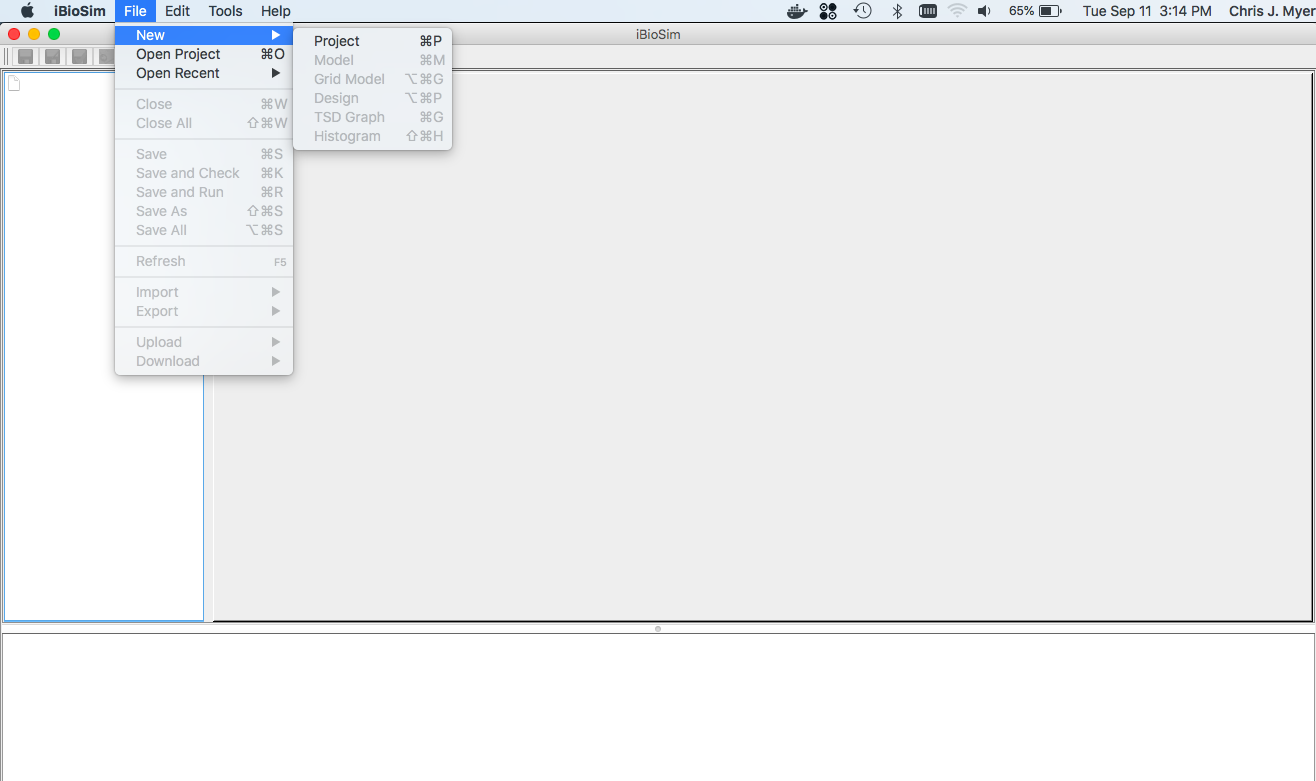
\includegraphics[width=160mm]{screenshots/project}
\end{center}

\item You will then be prompted to enter a Project ID.

\begin{center}
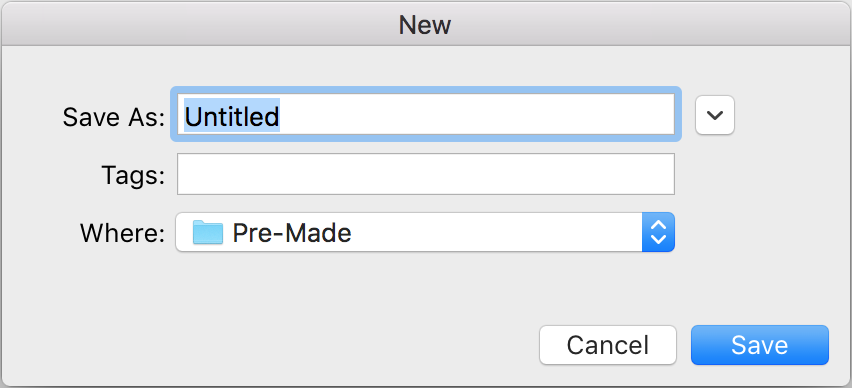
\includegraphics[width=75mm]{screenshots/ProjectIdGT}
\end{center}

\item Enter SynBioTutorial because this is Synthetic Biology Tutorial for iBioSim in order to create the project.

\begin{center}
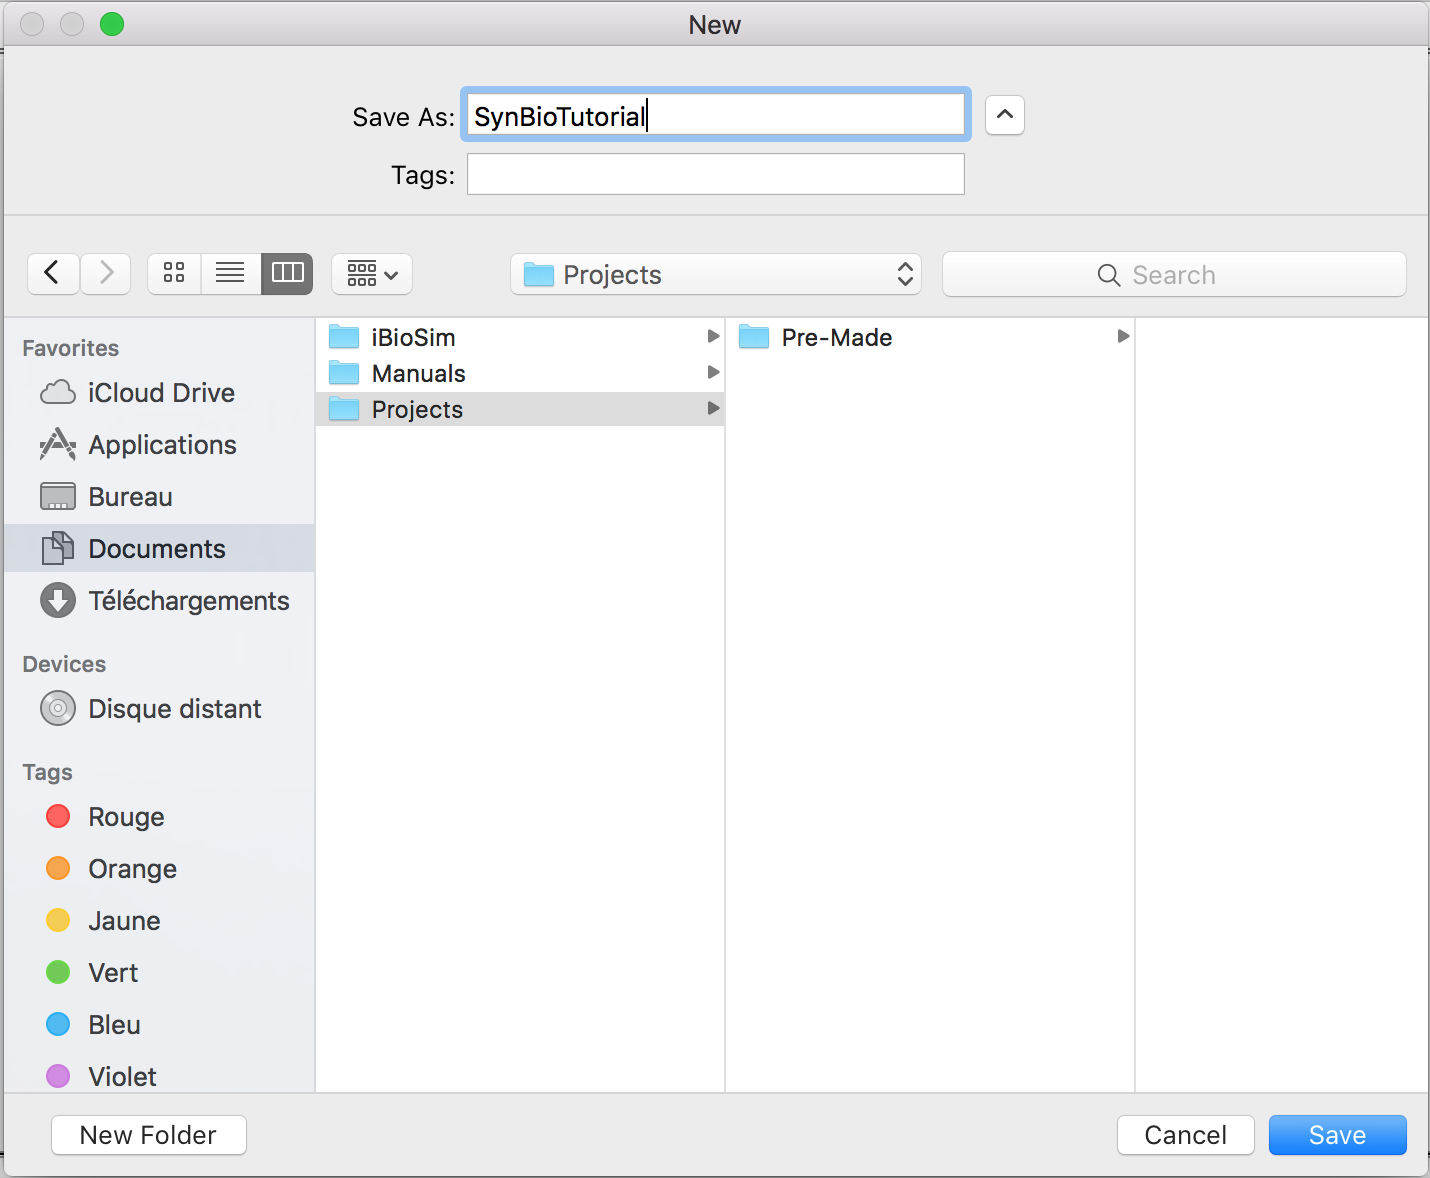
\includegraphics[width=110mm]{screenshots/ProjectIdGT2}
\end{center}

\end{itemize}

\section{Part Editor}
\subsection{LacI Inverter Gene}
\begin{itemize}
\item Before we can create our model for the Genetic Toggle Switch, we must first create the genetic circuits in the model. As aforementioned, there are two, the LacI repressible genes for TetR and GFP and the TetR repressible gene for LacI. These can be created using the Part Editor tool in this program, so select the File menu, hover over New, and select Part.

\begin{center}
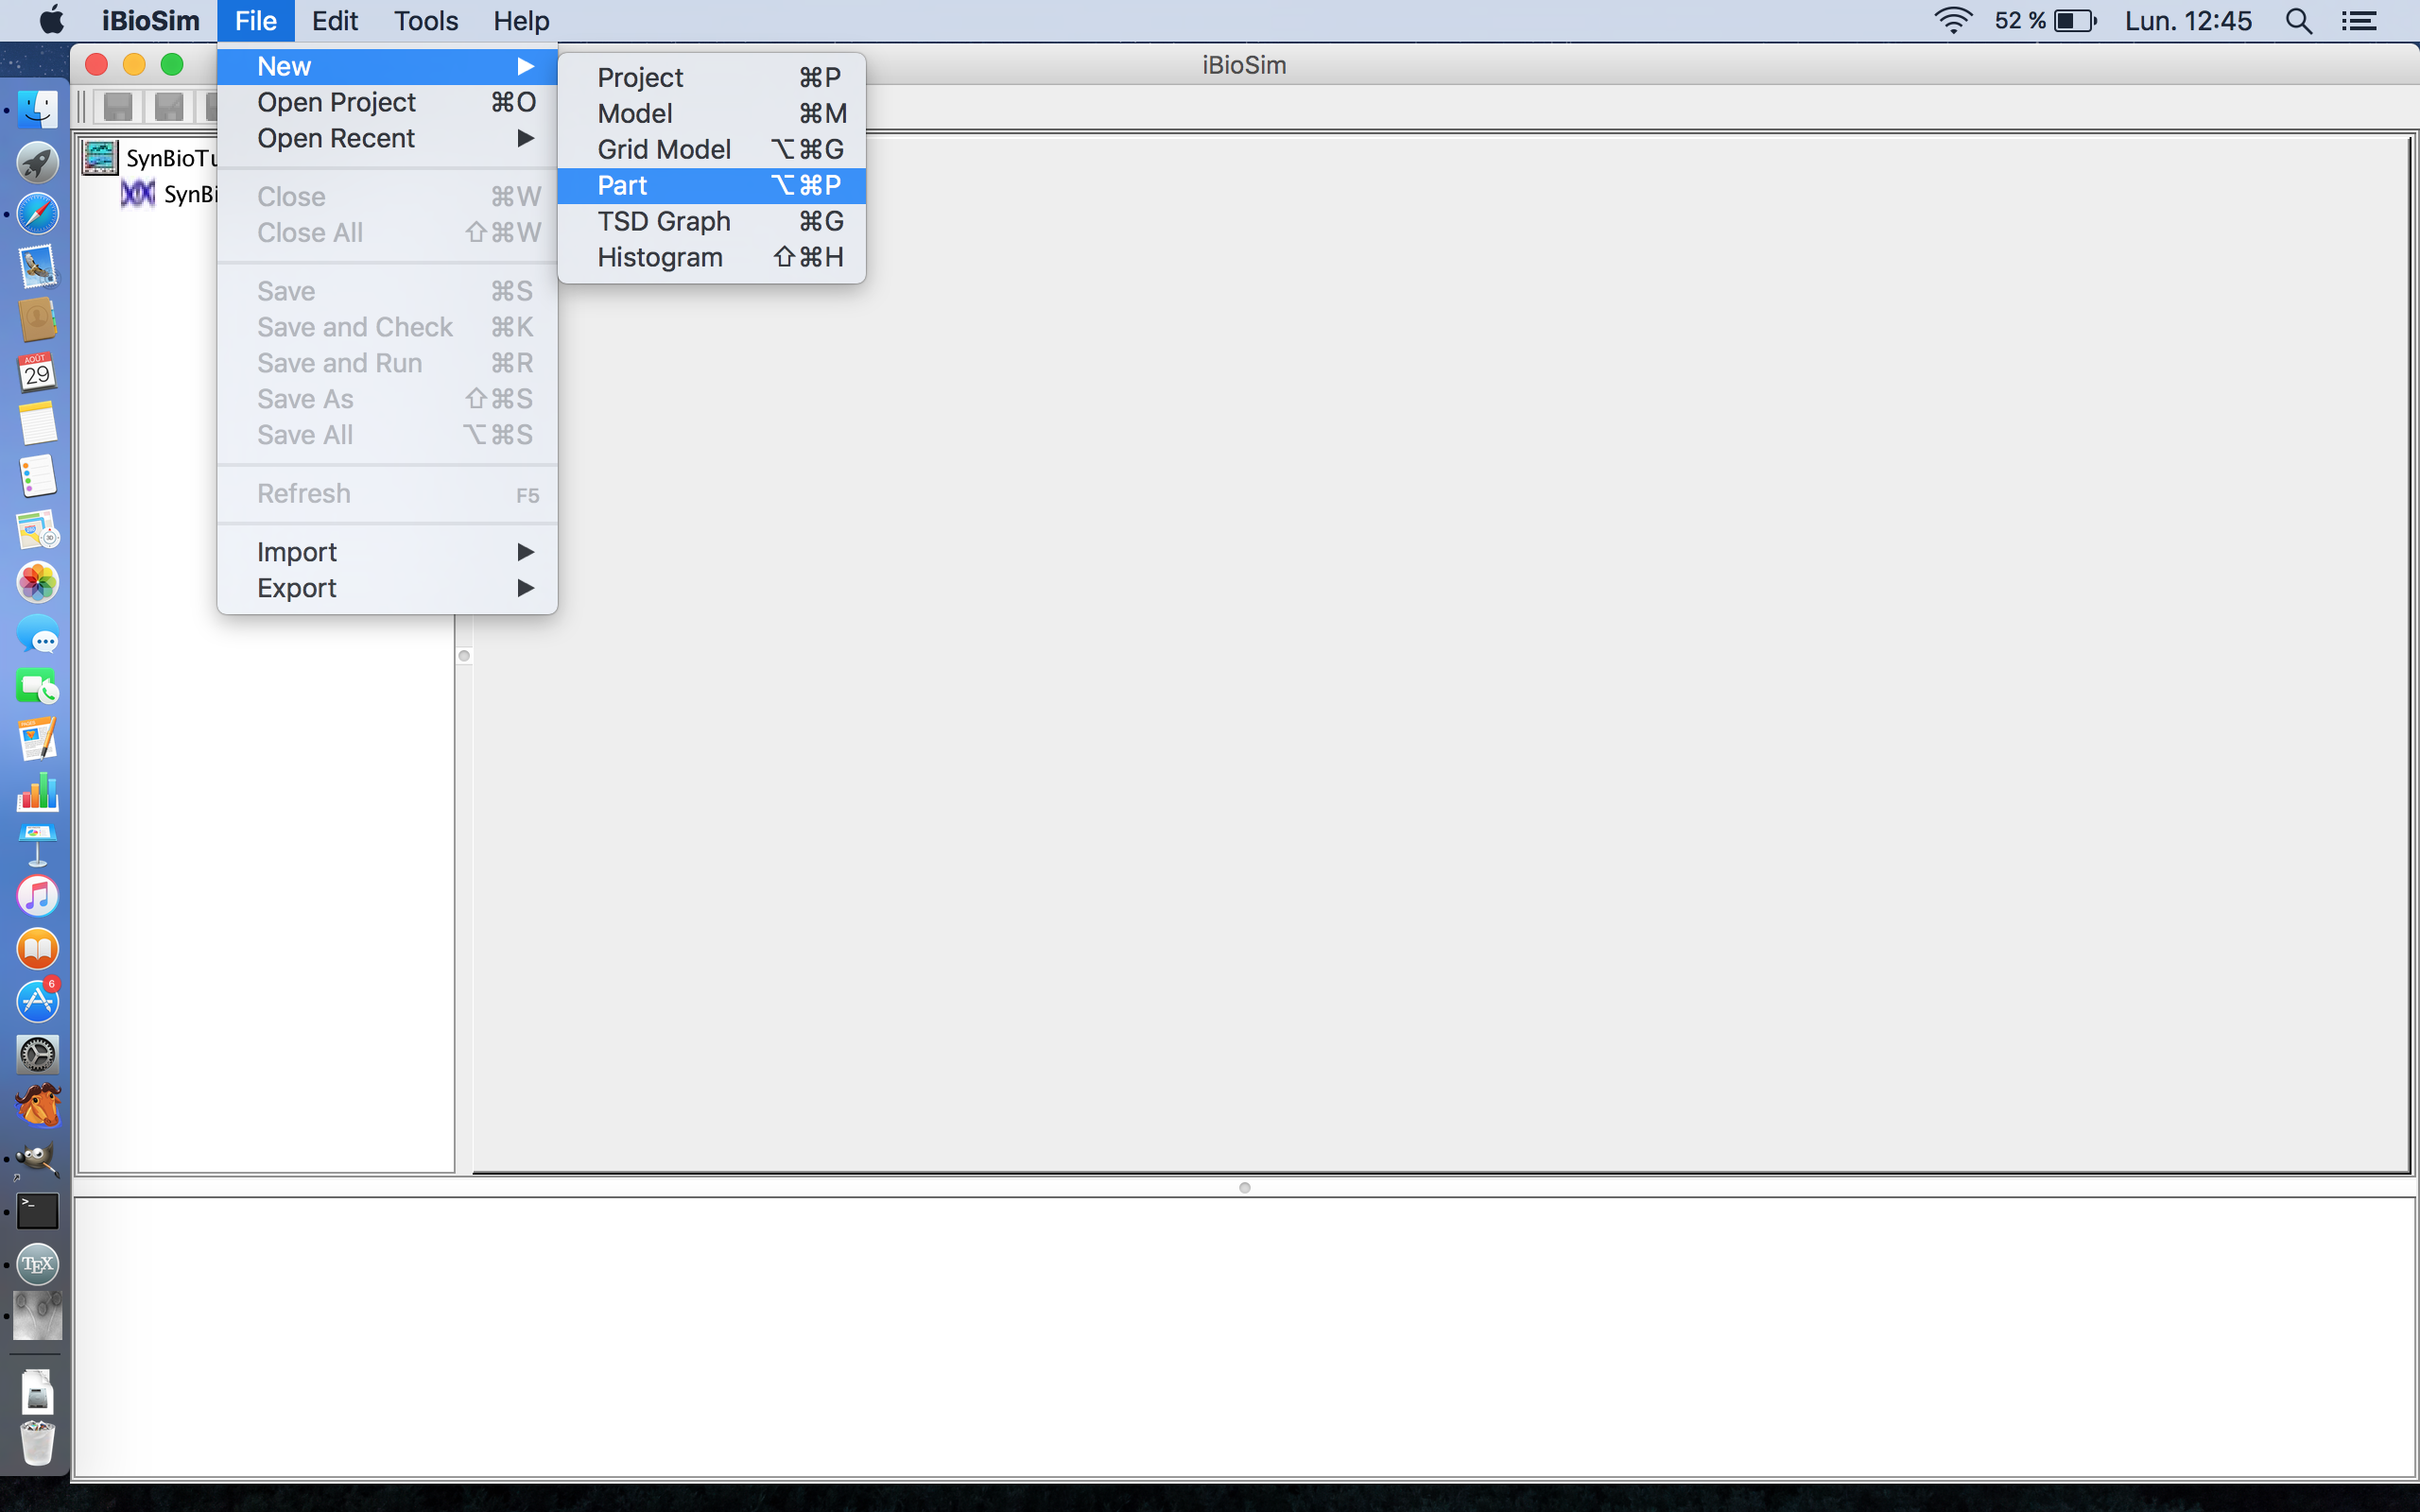
\includegraphics[width=160mm]{screenshots/newPart}
\end{center}

\item You will then be prompted to enter a Part ID for this circuit. This tutorial will start with the circuit for the LacI repressible genes for TetR and GFP, so enter LacI\_Inverter\_Gene into the Part ID. 

\begin{center}
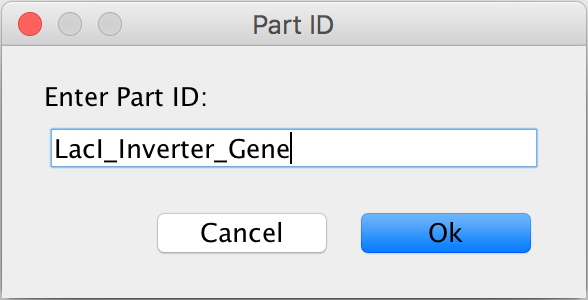
\includegraphics[width=75mm]{screenshots/PartIdGT}
\end{center}

\item This will then open up the Part Editor allowing us to begin to create the genetic circuit. The first part of this circuit like many circuits is a promoter, which is where transcription of genes begin, so click the promoter icon to add it to the circuit. The promotor icon is the second icon from the left on the part ribbon.

\begin{center}
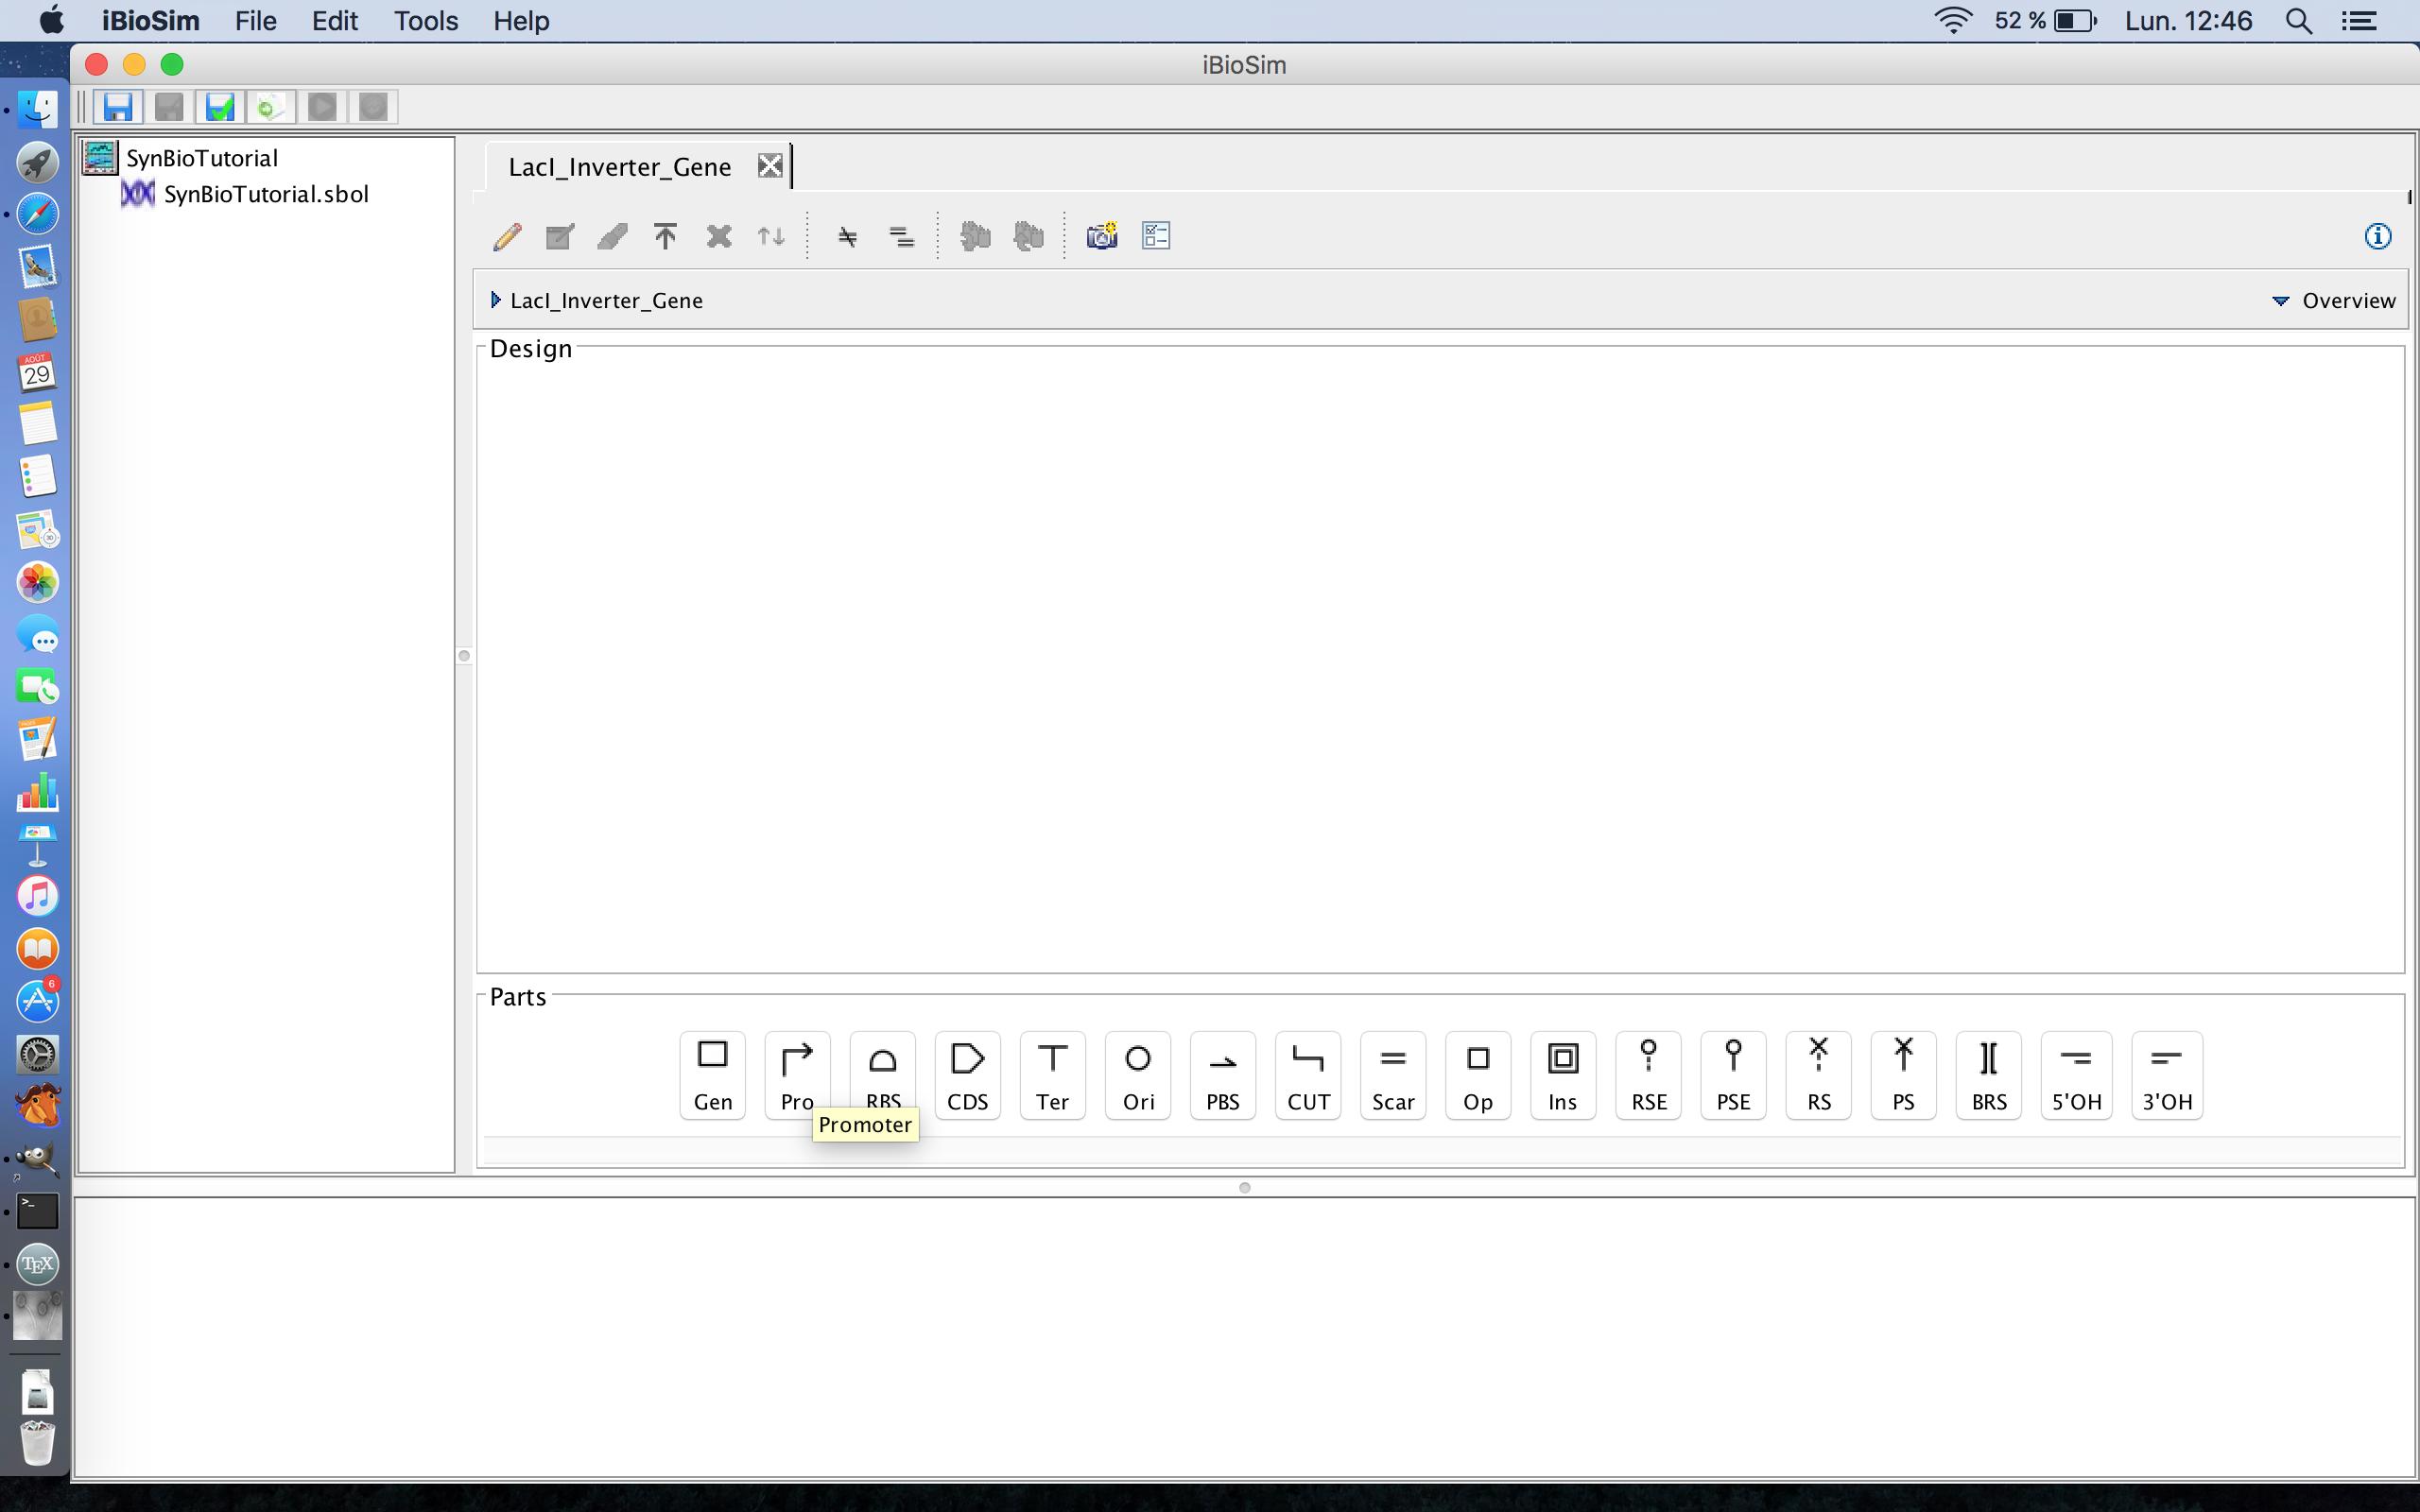
\includegraphics[width=160mm]{screenshots/PartPromoter}
\end{center}

\item The next part of this circuit is the TetR gene, so select the gene icon to add the TetR gene to the circuit. This will then open the Gene Editor. The gene icon is the first icon from the left on the part ribbon.

\begin{center}
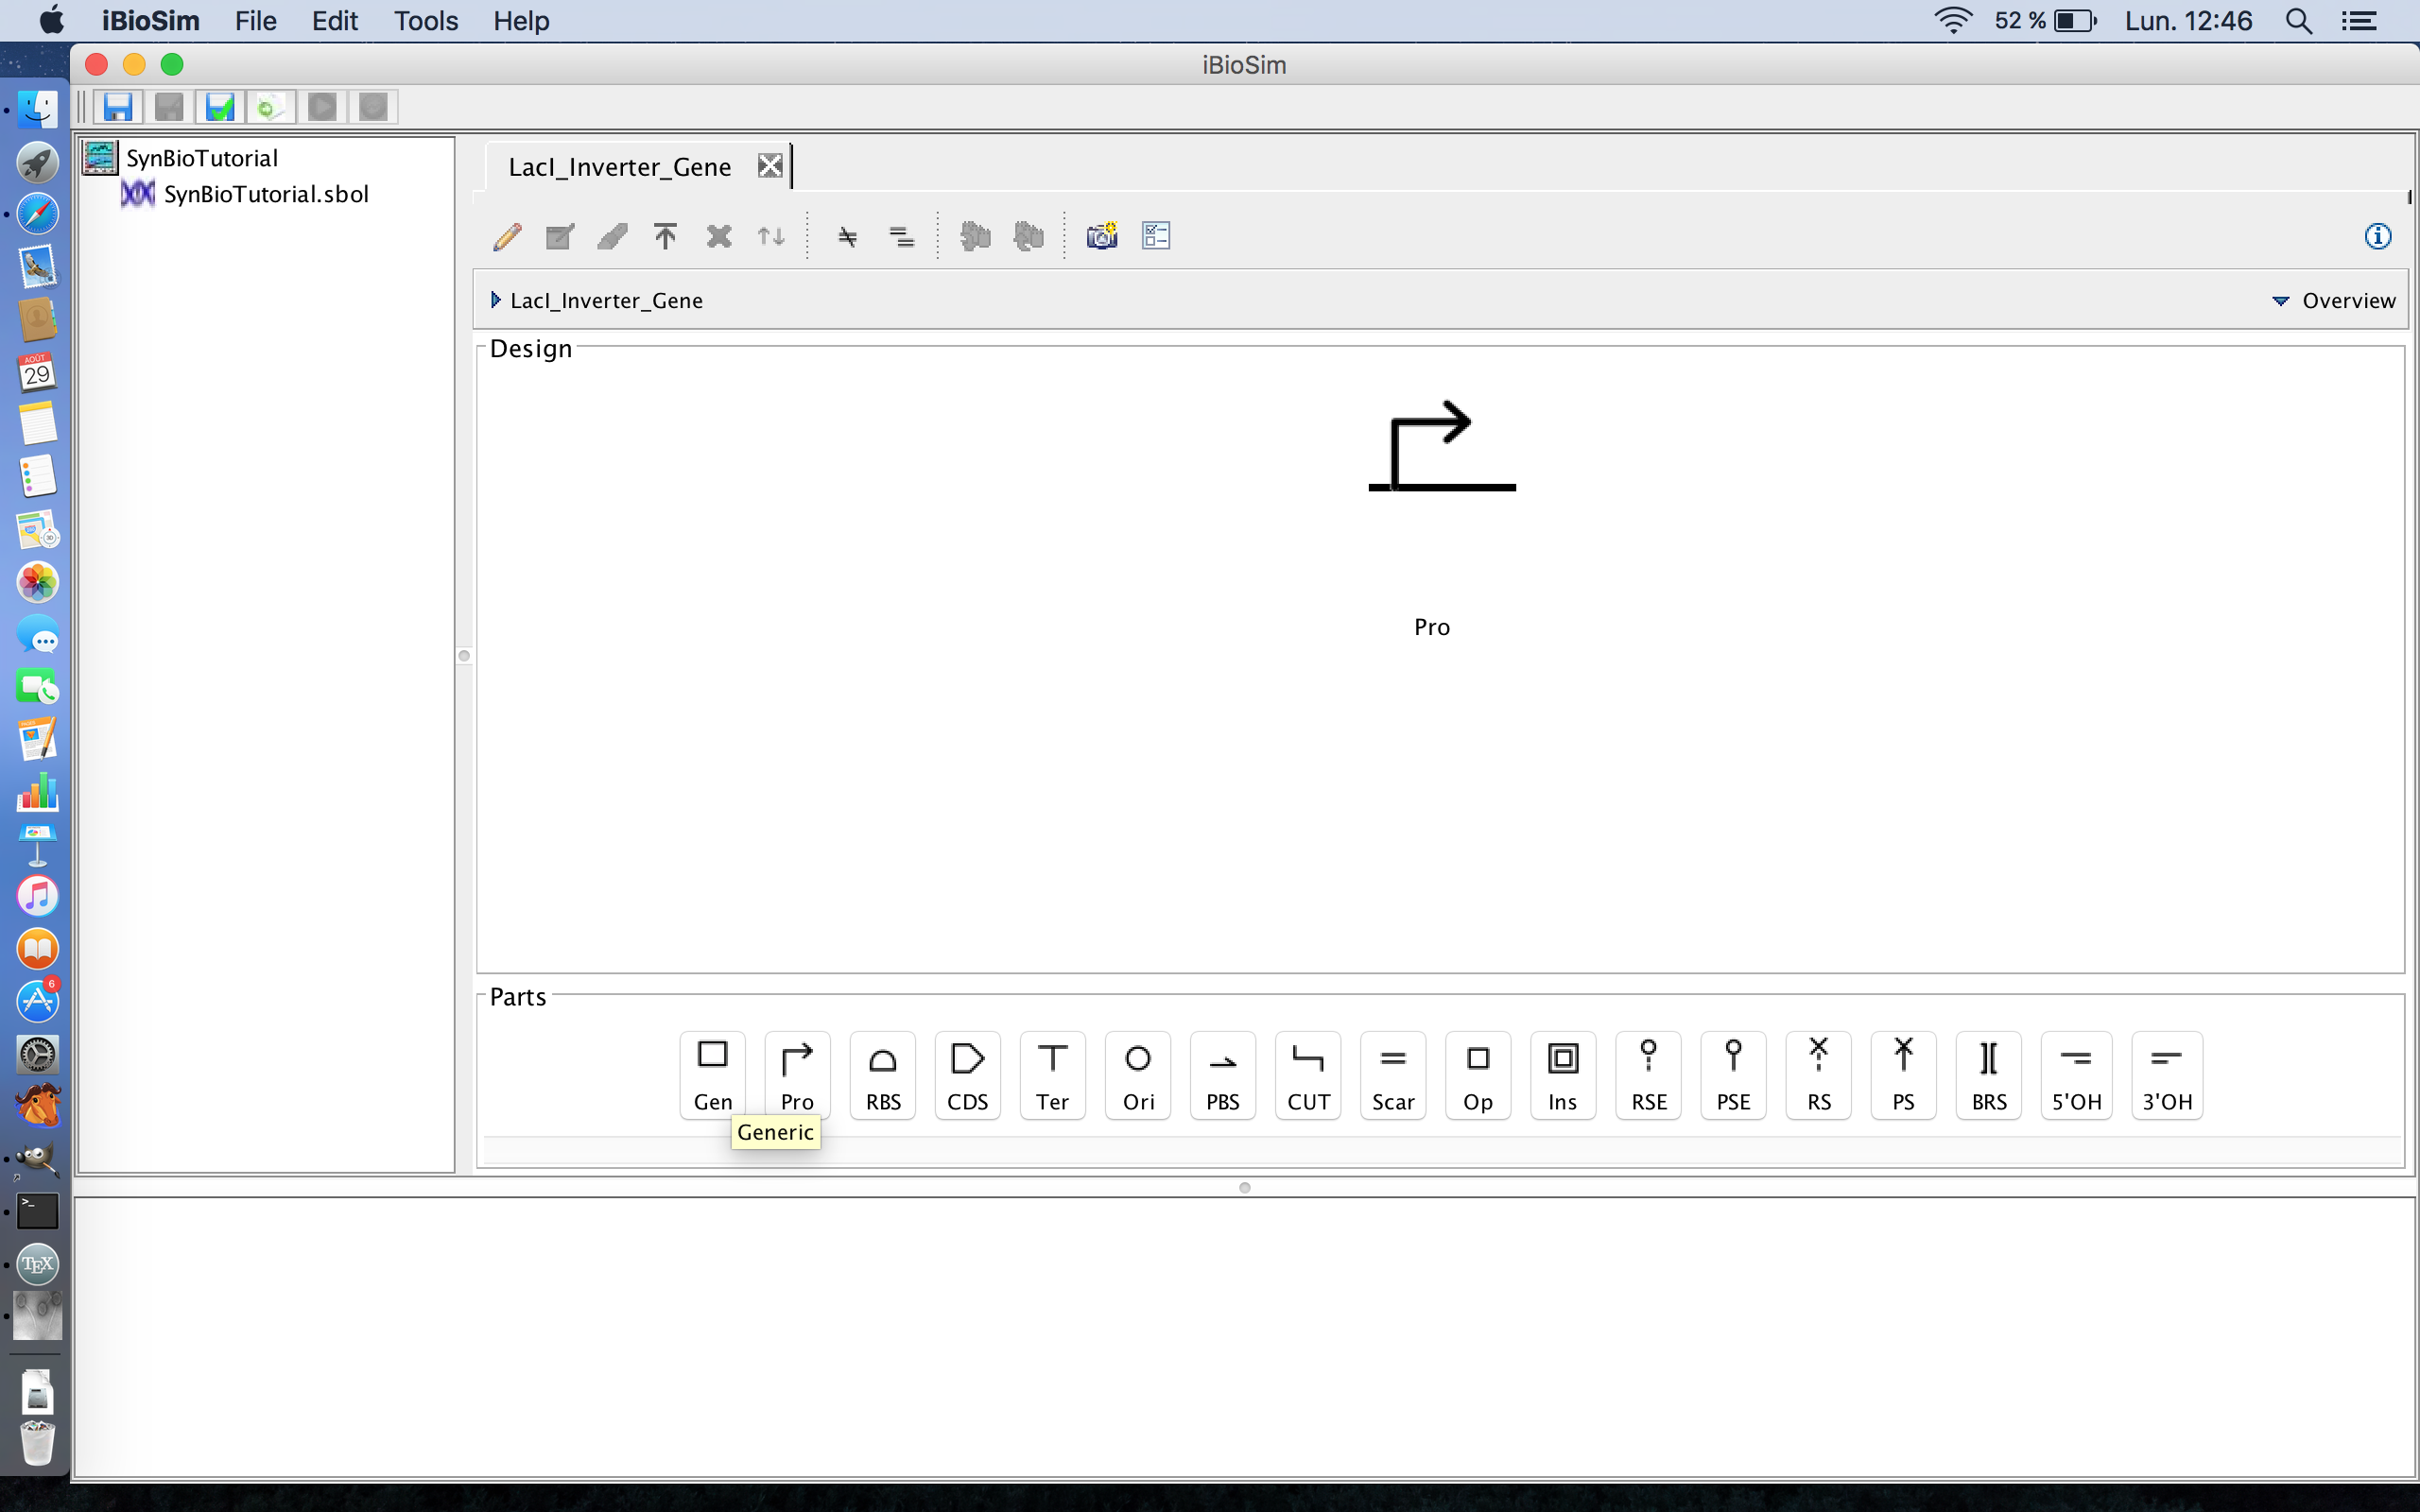
\includegraphics[width=160mm]{screenshots/PartGene}
\end{center}

\begin{center}
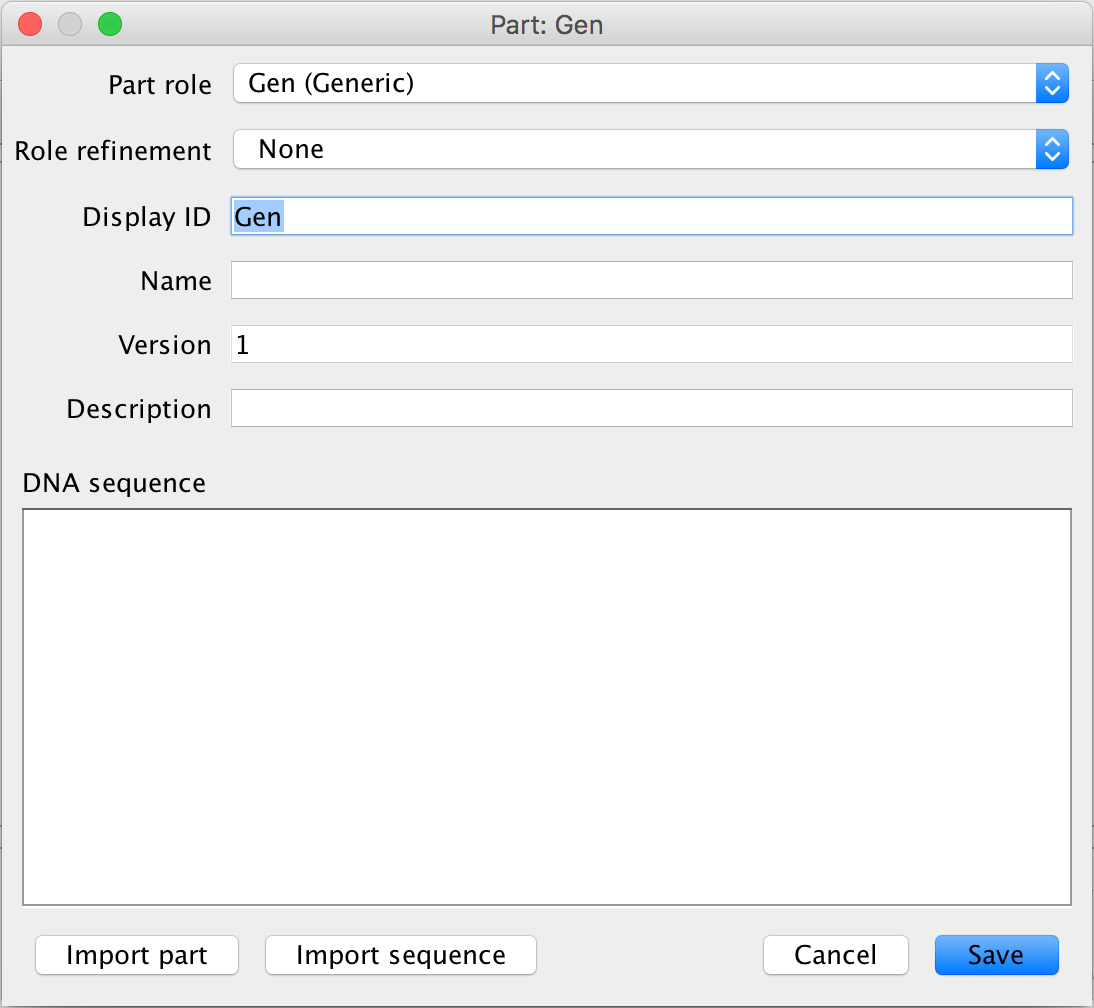
\includegraphics[width=110mm]{screenshots/PartGeneEditor}
\end{center}

\item Since this is the TetR gene, enter TetR\_Gene into the Display ID and click Ok to add the gene to the circuit.

\begin{center}
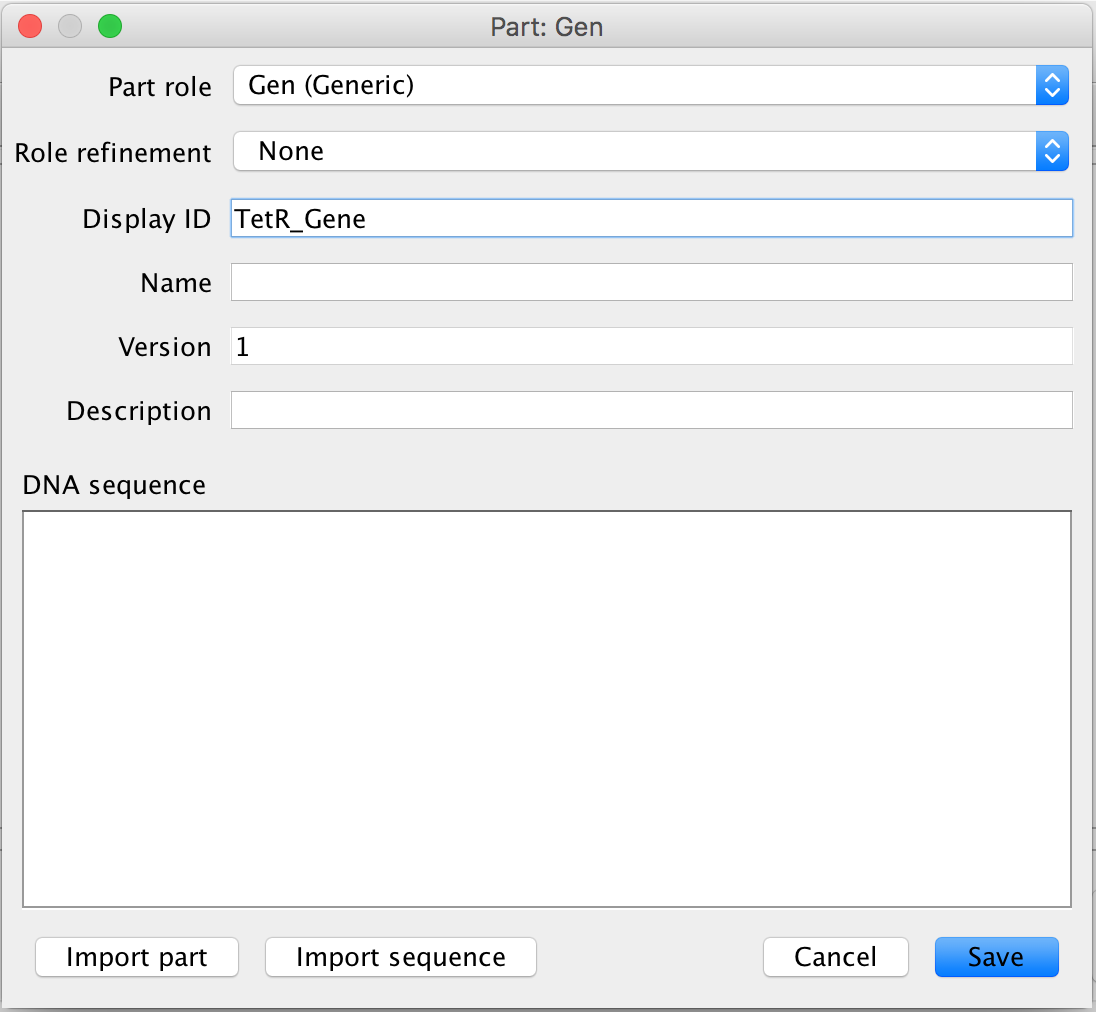
\includegraphics[width=110mm]{screenshots/PartTetRGene}
\end{center}

\item Now, do the exact same thing as above to add the GFP gene to the circuit.

\begin{center}
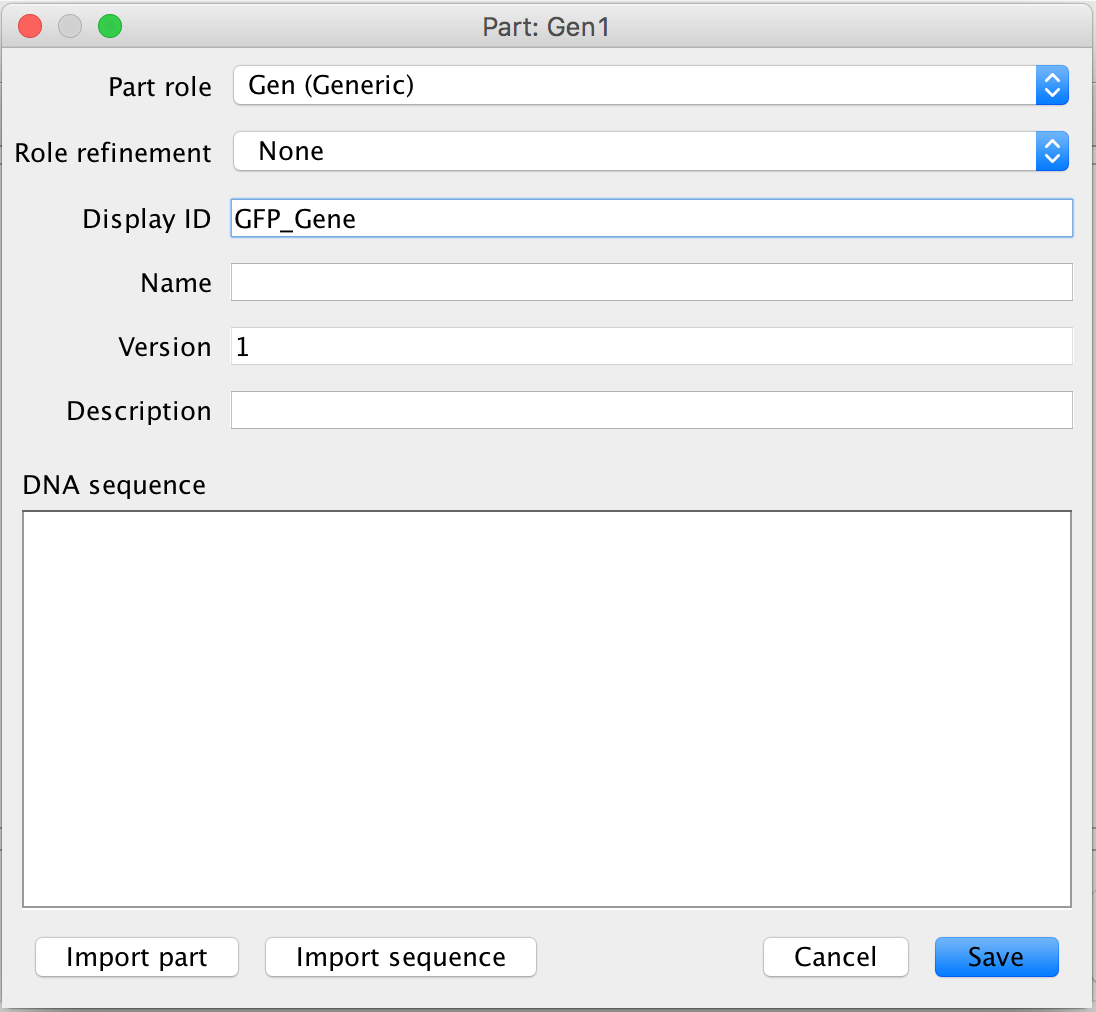
\includegraphics[width=110mm]{screenshots/PartGFPGene}
\end{center}

\item The next step is to add the terminator to the circuit, which is where transcription ends, so click the terminator icon to add it to the circuit. The terminator icon is the fifth icon from the left on the part ribbon.

\begin{center}
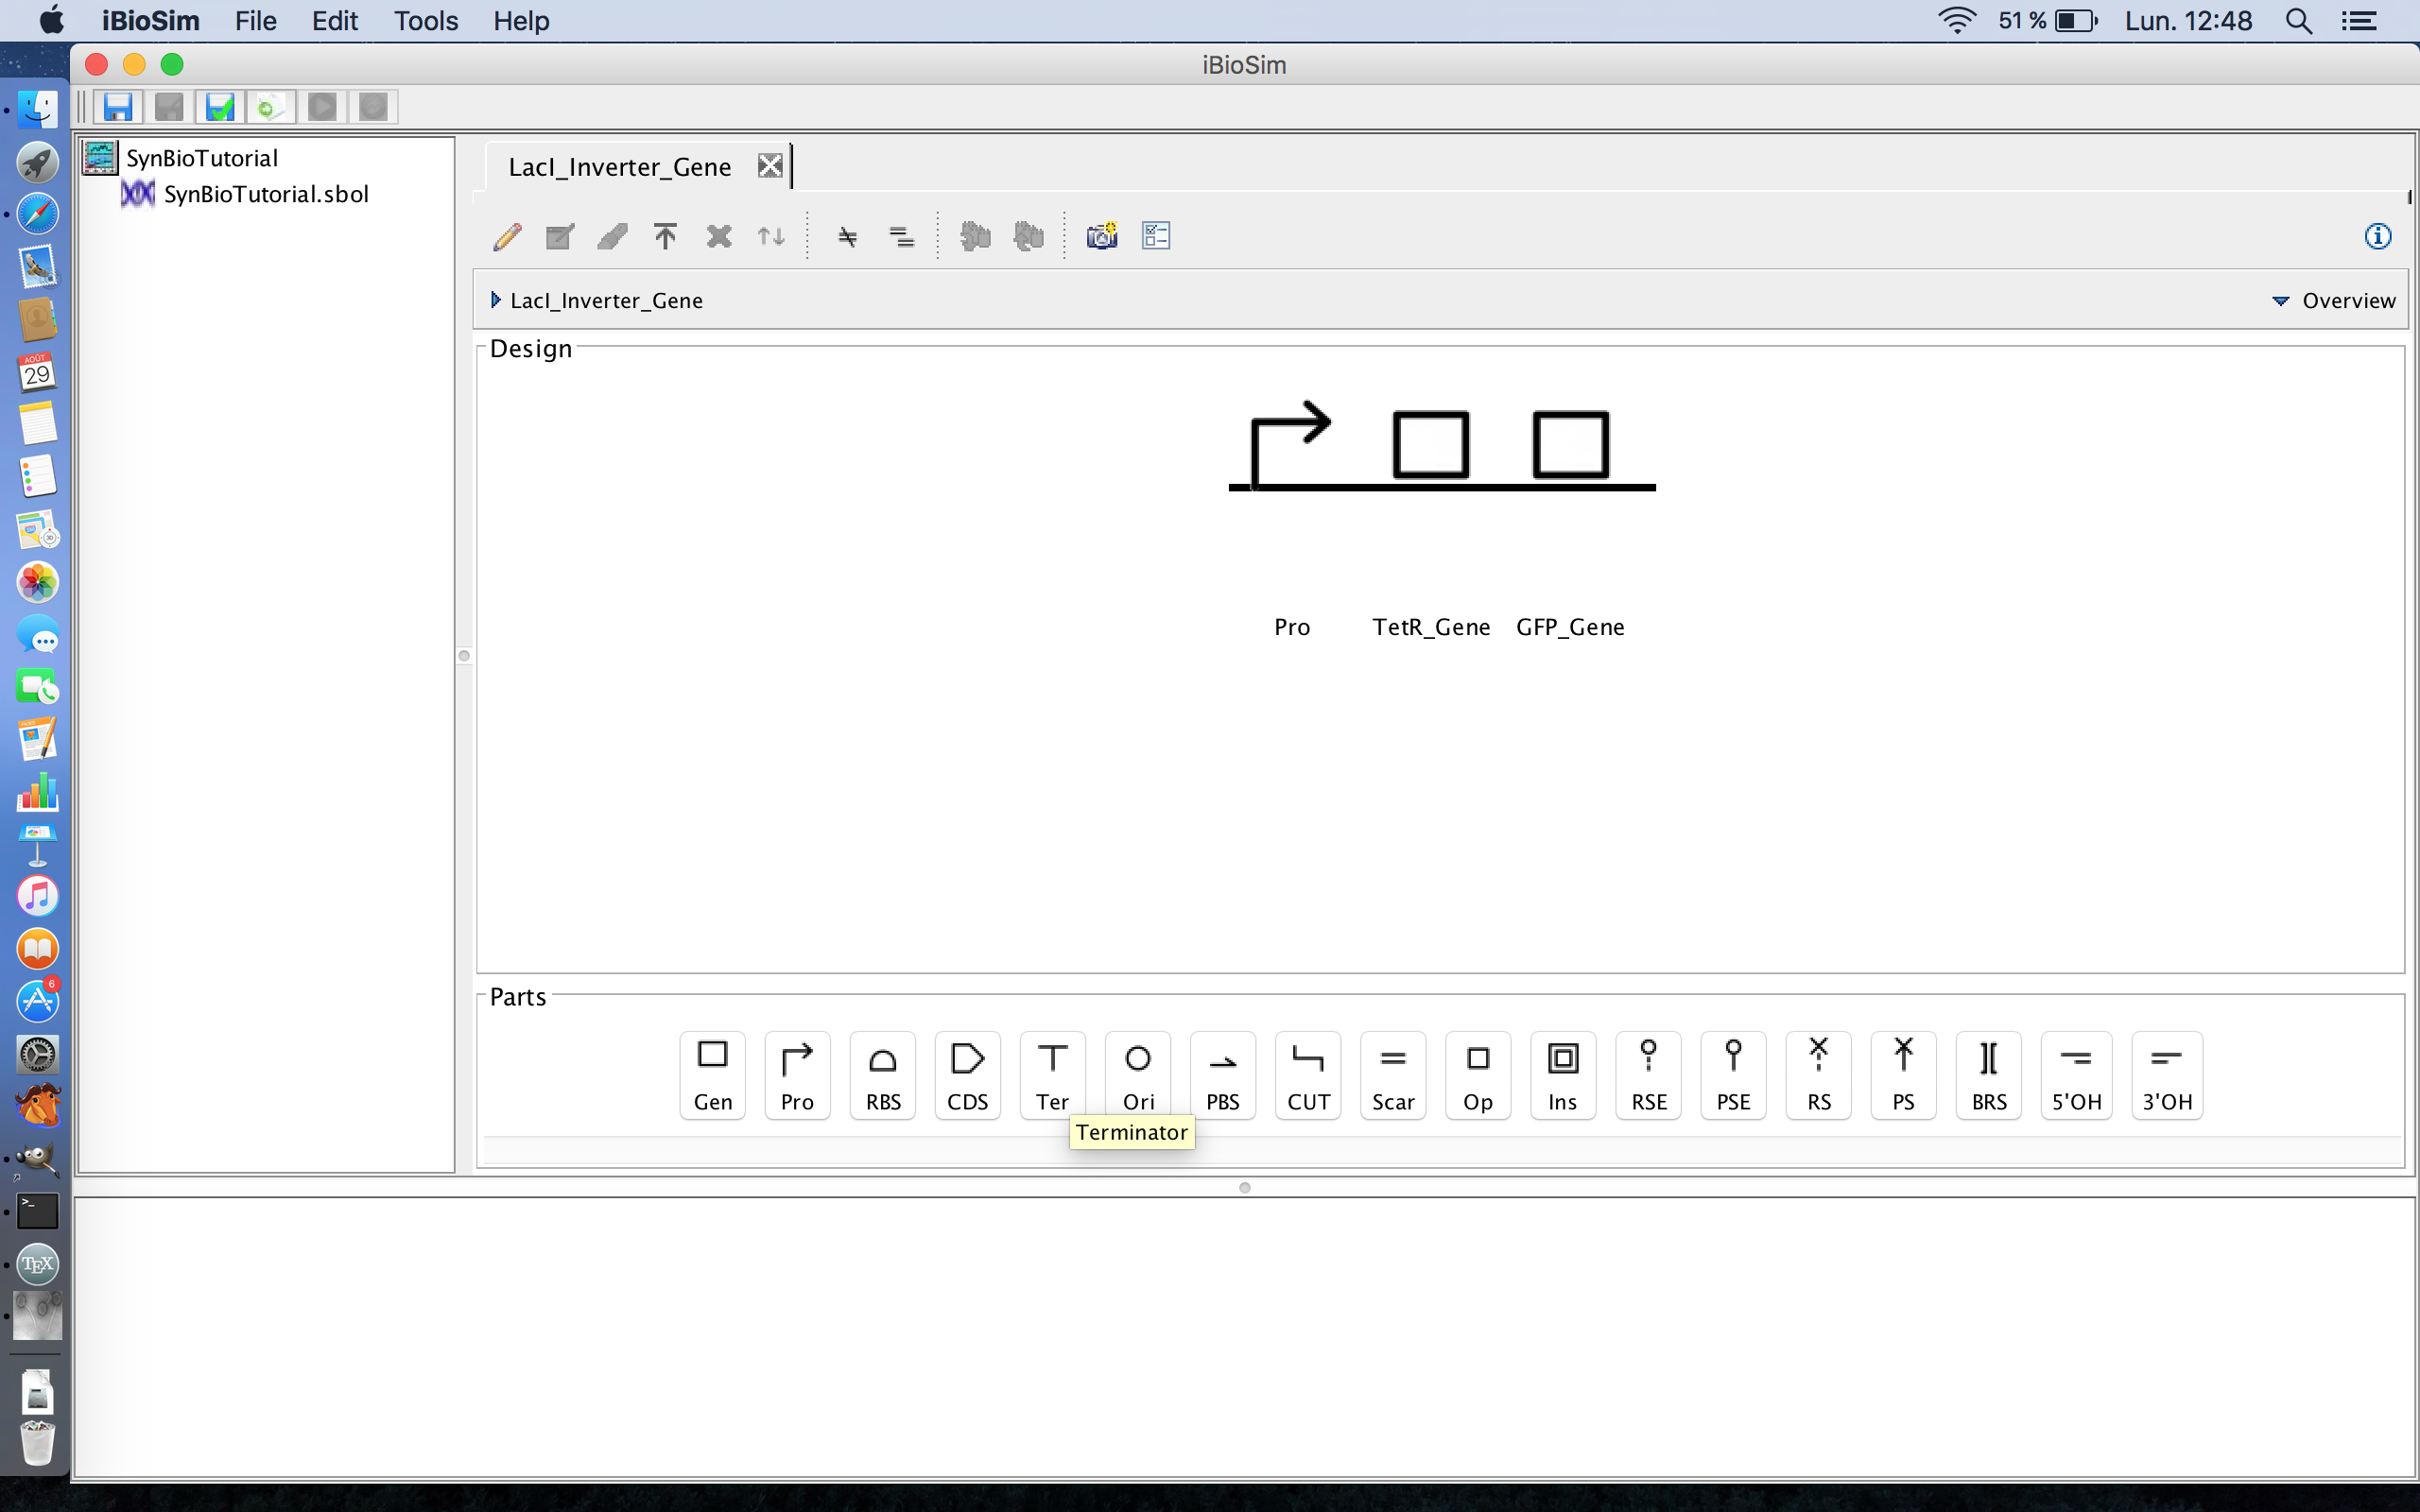
\includegraphics[width=160mm]{screenshots/PartTerminator}
\end{center}

\item Now that the framework for this genetic circuit is laid out, it is now time to begin adding some of the details. The first step of which is to expand the genes, so select the TetR gene and the focus in icon from the tool ribbon. The focus in icon is the fourth icon from the right.

\begin{center}
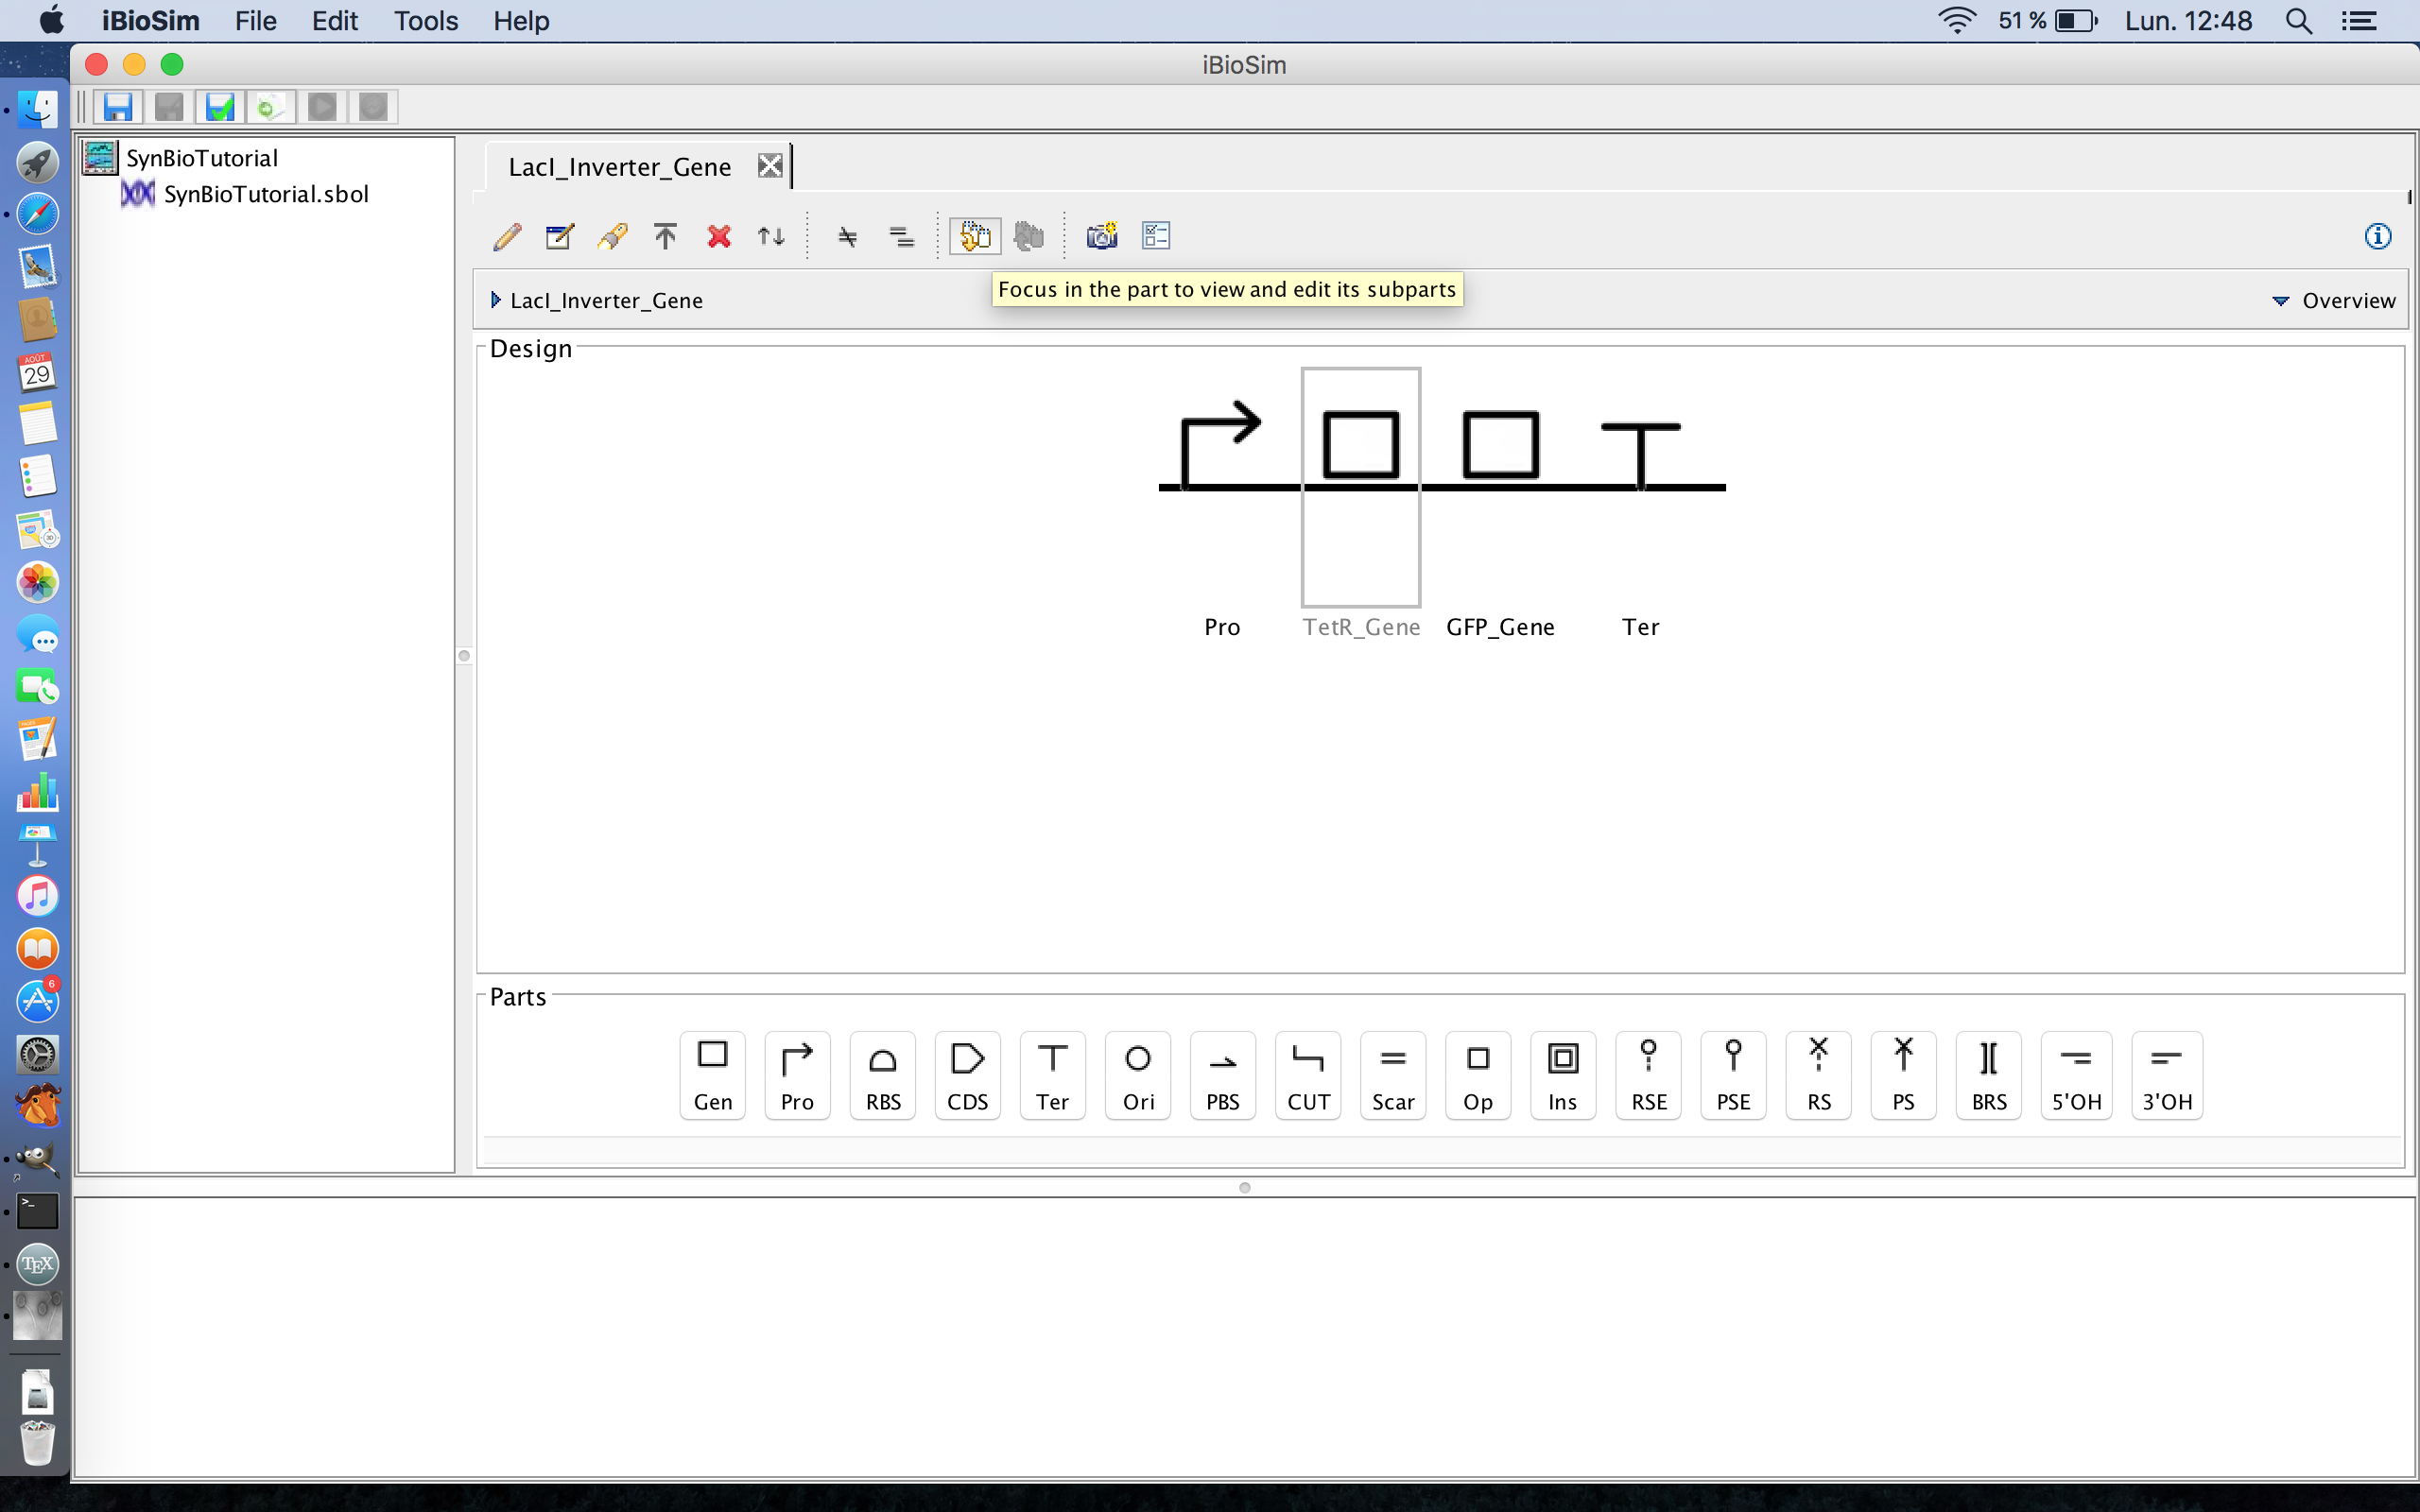
\includegraphics[width=160mm]{screenshots/PartFocusIn}
\end{center}

\item Now we can add the components of the TetR gene itself to the genetic circuit. Like all coding sequences, the TetR gene has a ribosome binding site where the ribosome binds during translation, so click the ribosome binding site icon to add it to the genetic circuit. The ribosome binding site icon is the third icon from the left on the part ribbon.

\begin{center}
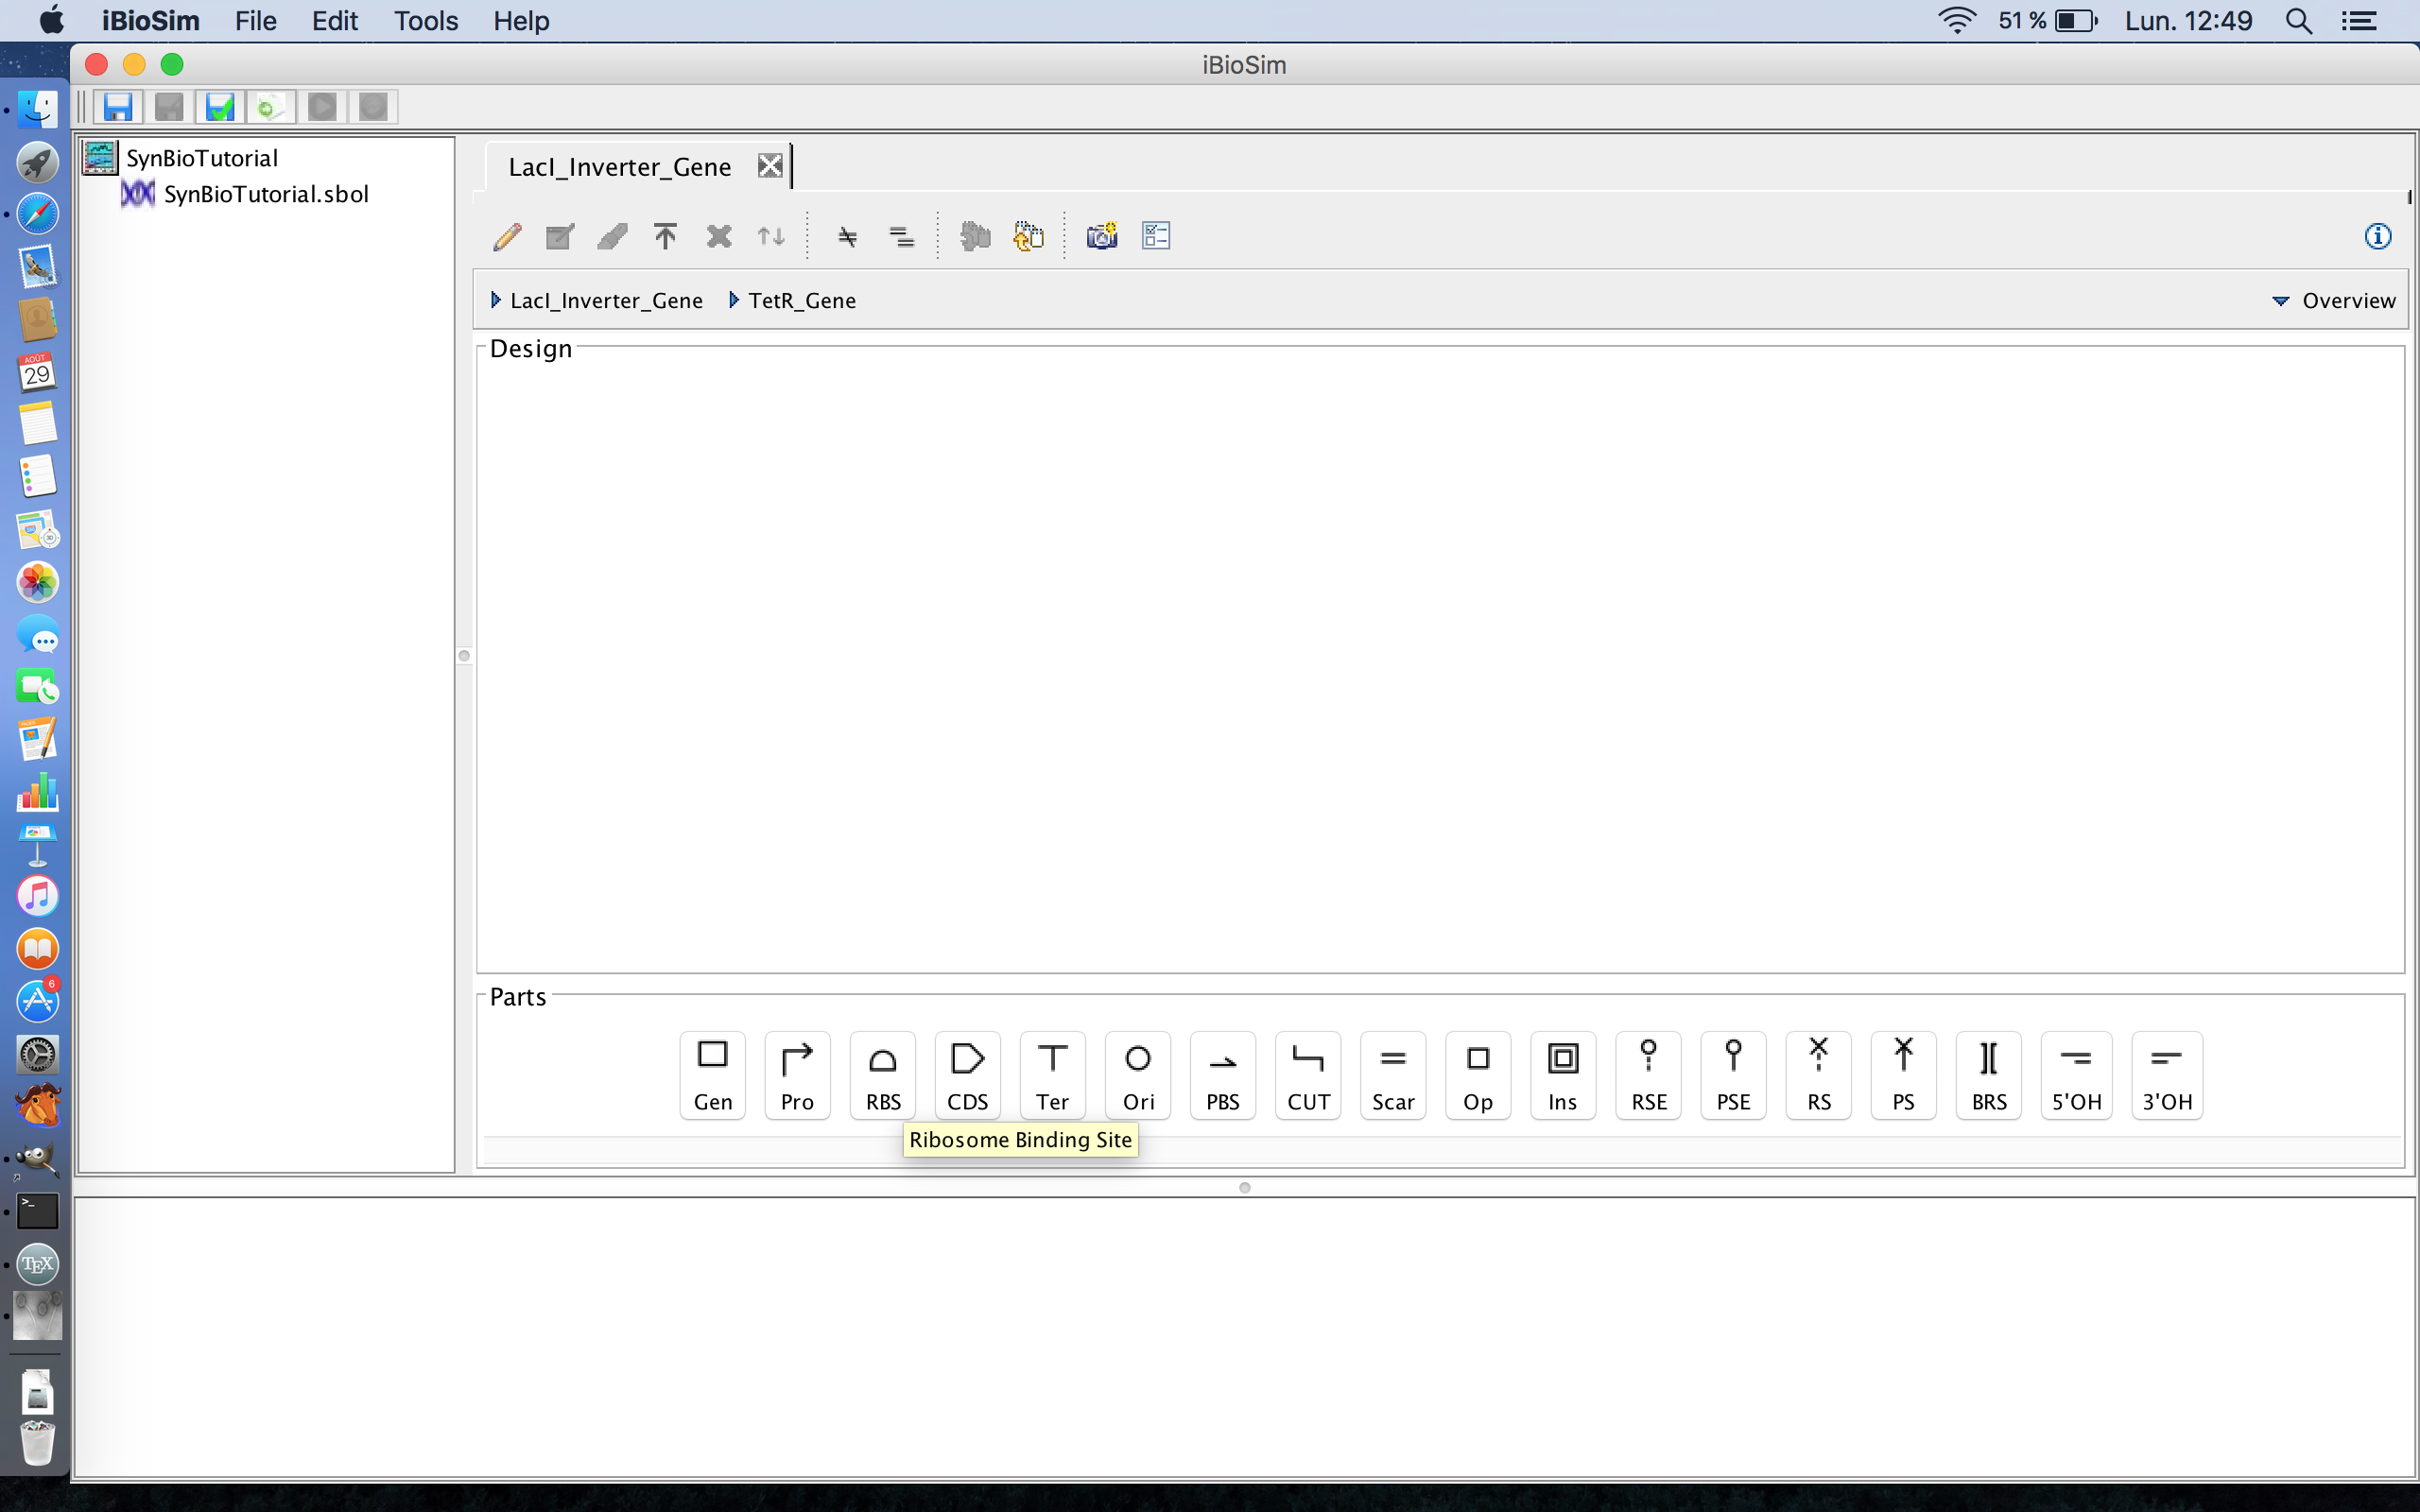
\includegraphics[width=160mm]{screenshots/PartRBS}
\end{center}

\item The next part in genes after the ribosome binding site is the coding the sequence, the part of the gene that codes for the TetR protein, so click the coding sequence icon to add it to the genetic circuit. The coding sequence icon is the fourth icon from the left on the part ribbon.

\begin{center}
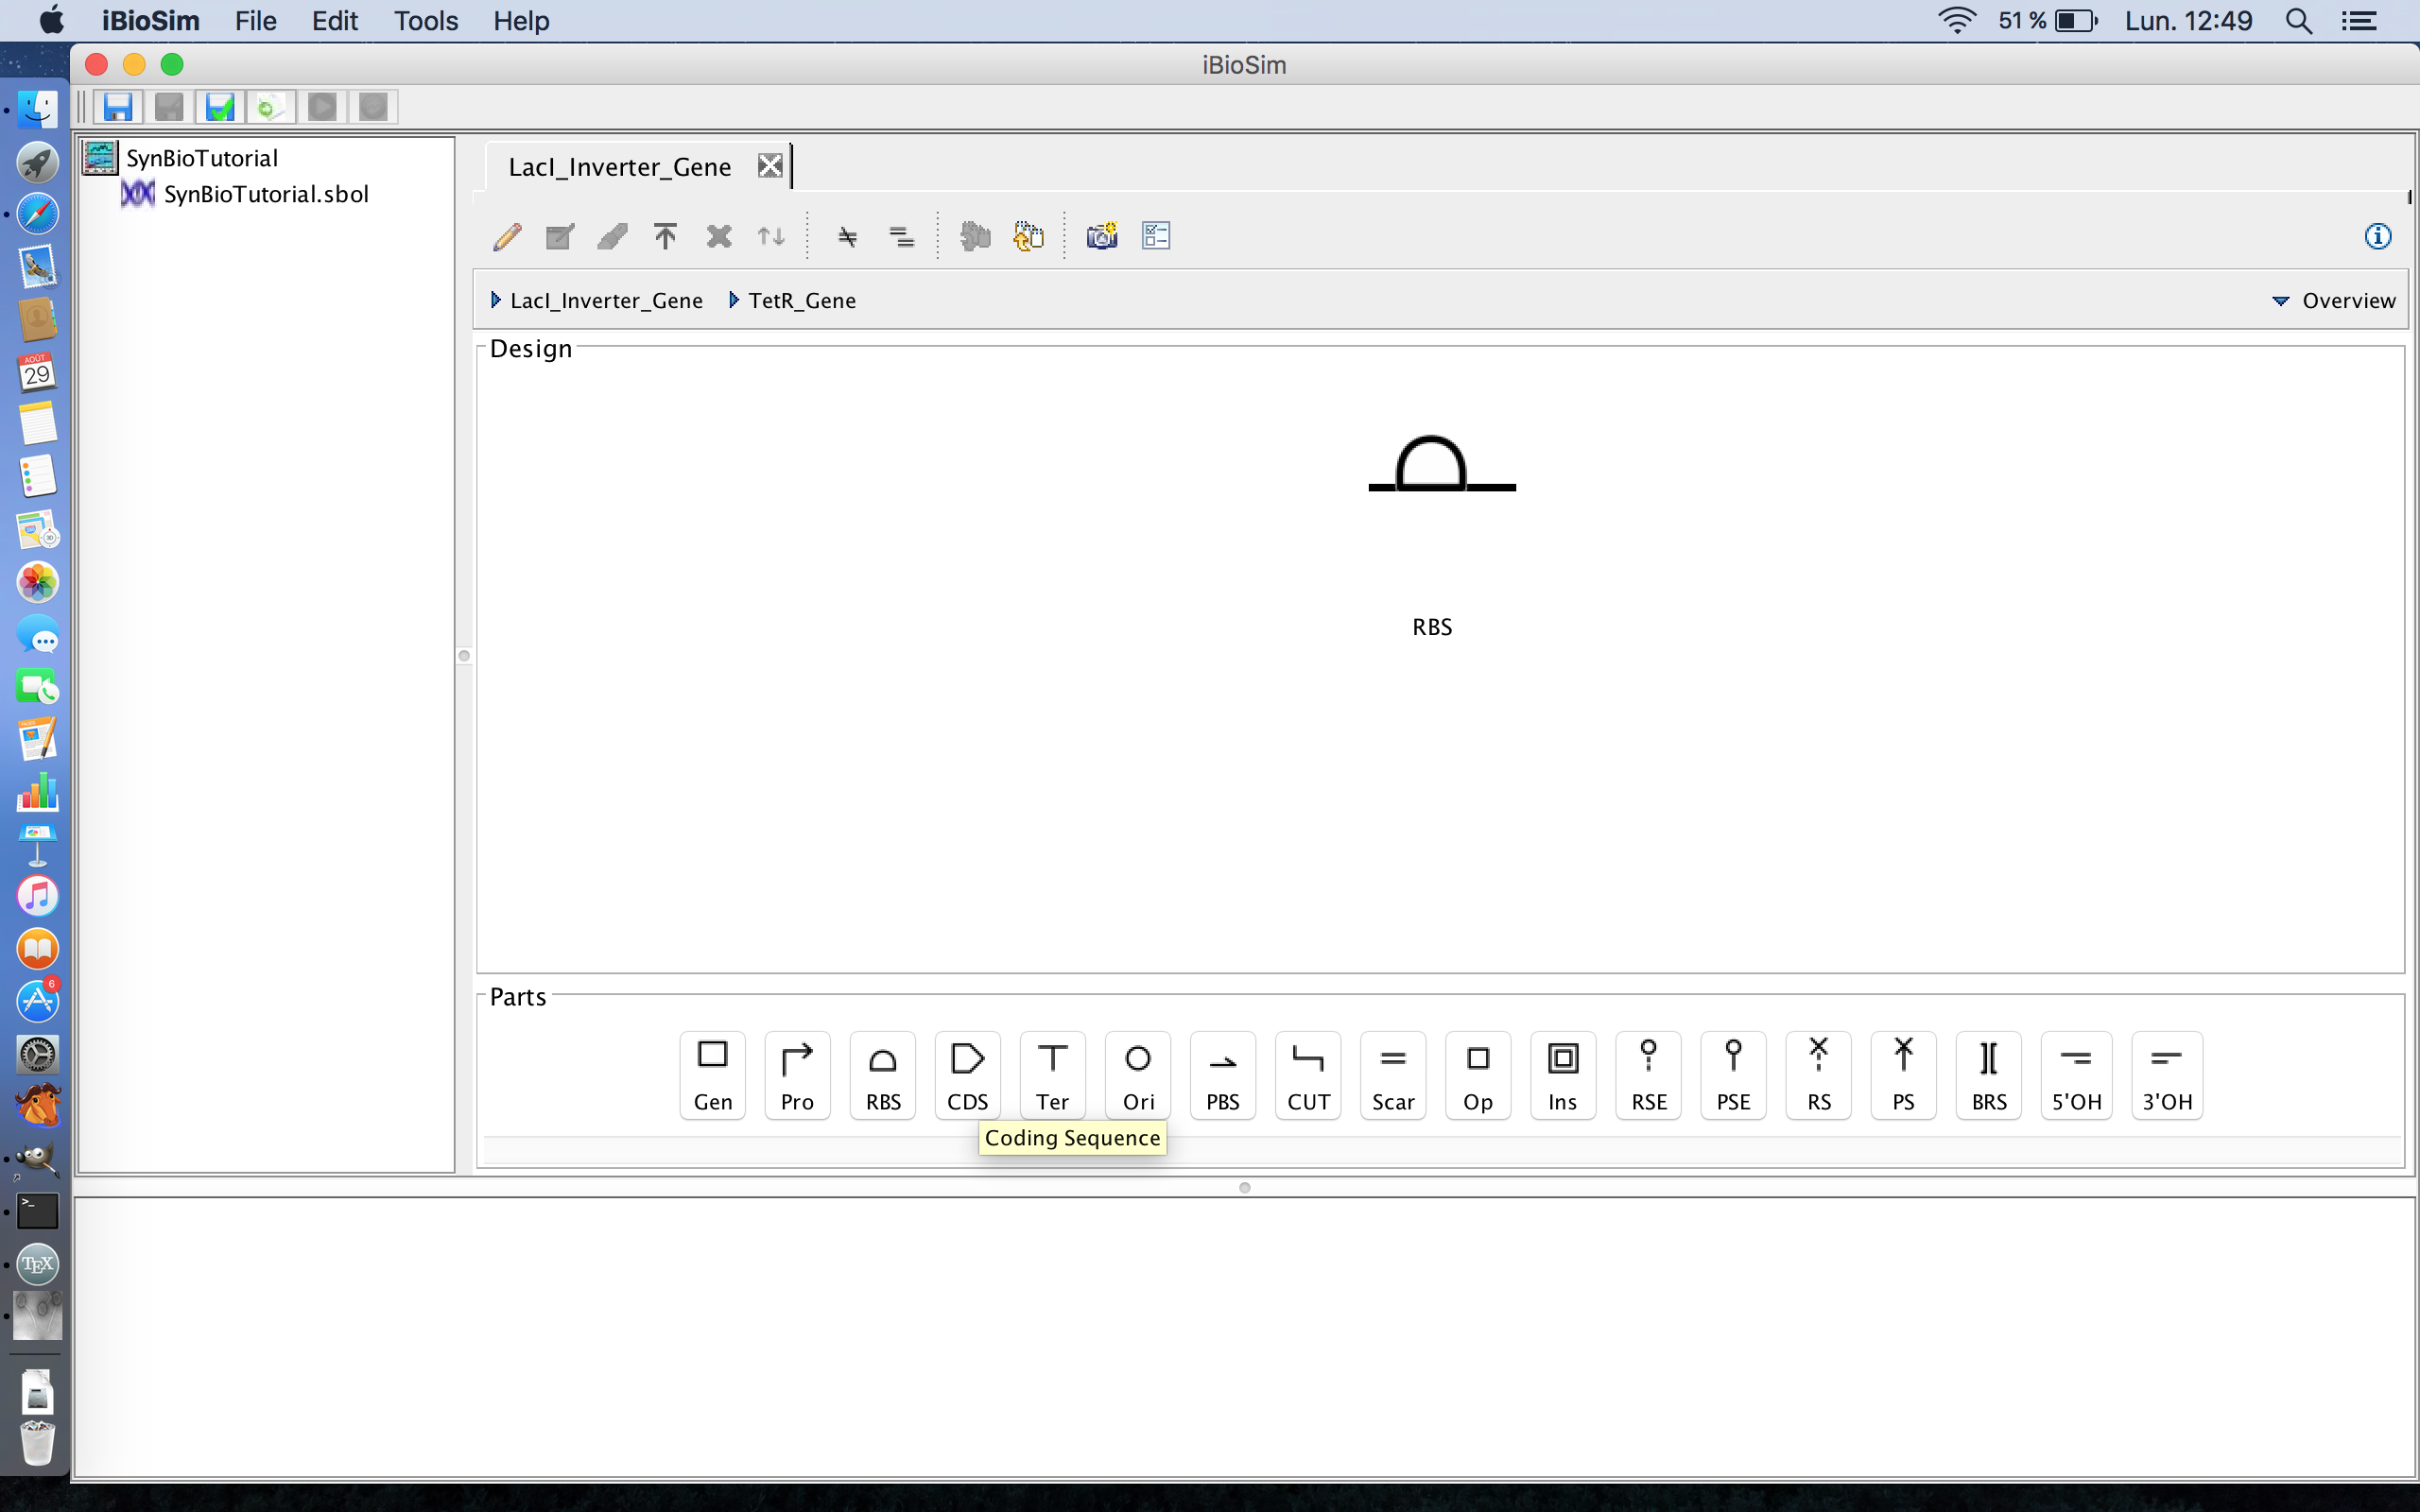
\includegraphics[width=160mm]{screenshots/PartCDS}
\end{center}

\item Now that we have the parts of the TetR gene, it is time to associate the parts of the gene with the actual DNA sequences that code for these parts of the gene. This is possible due to the SBOL library in Newcastle University, UK. Note, this part of the tutorial requires an internet connection in order to access the library, so lets start by selecting the ribosome binding site and clicking the search part registry icon. The search part registry icon is the third icon from the left on the tool ribbon.

\begin{center}
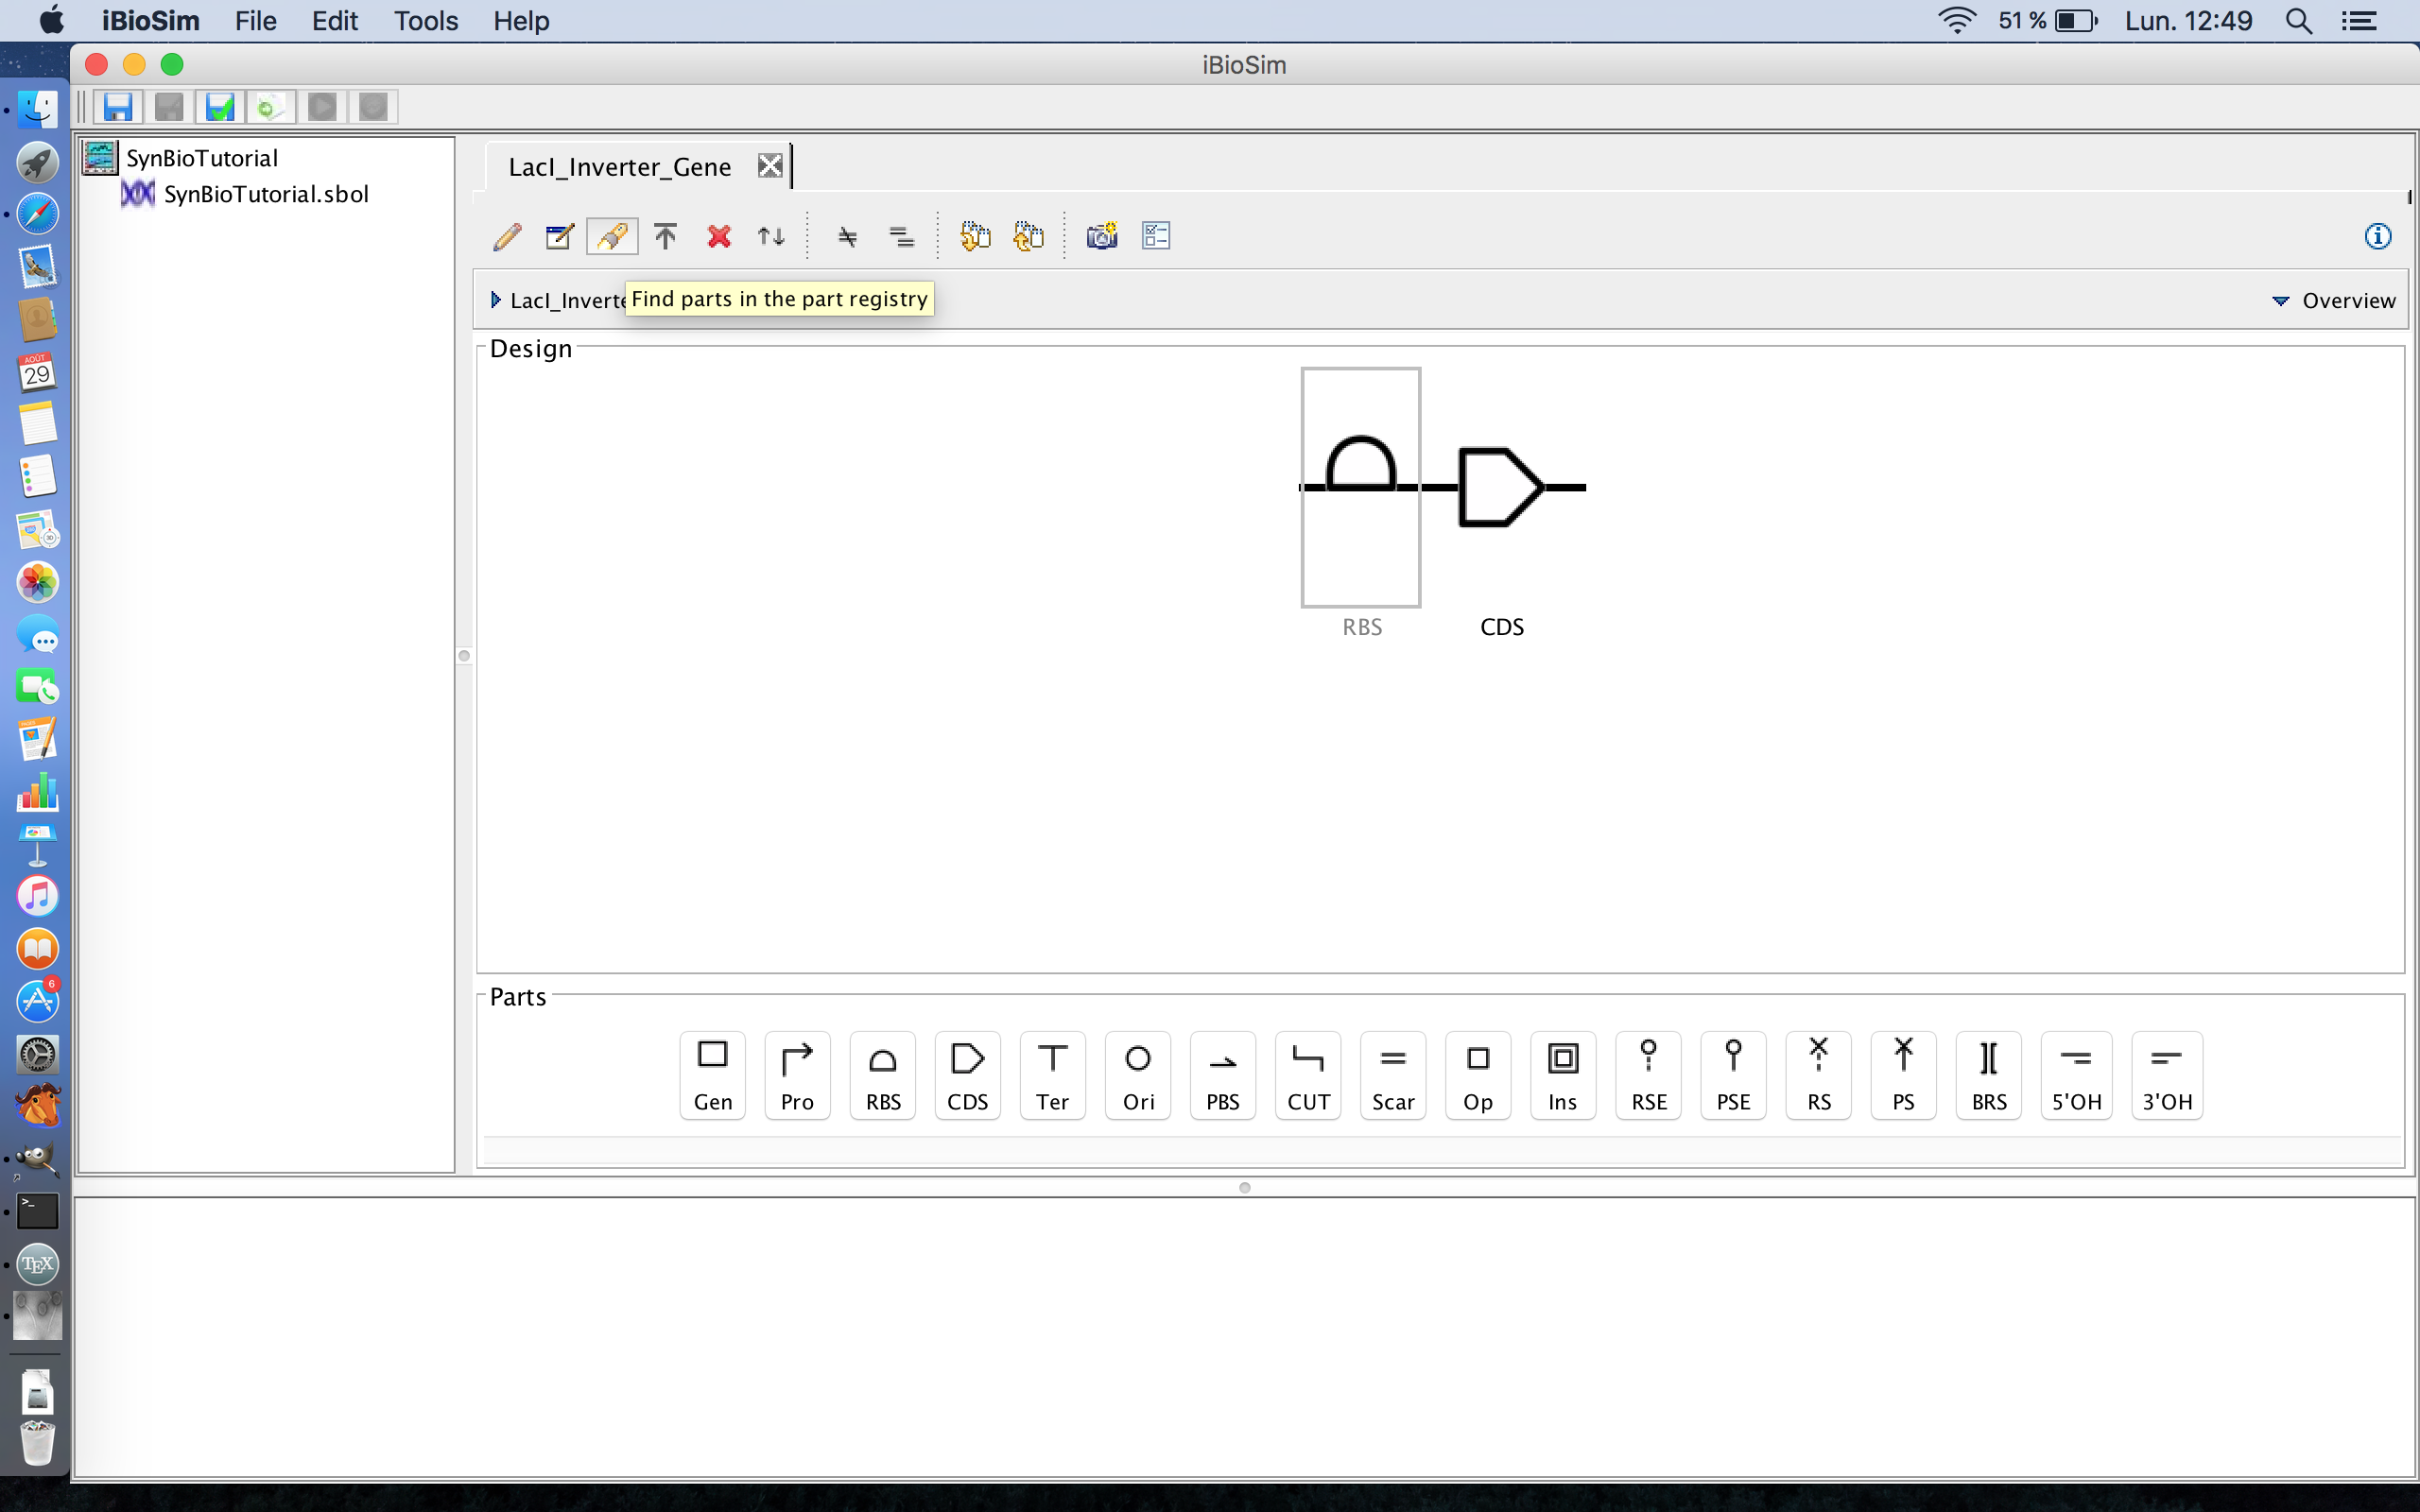
\includegraphics[width=160mm]{screenshots/PartSearchPartRegistry}
\end{center}

\item Clicking the search part registry icon opens the Part Registry. First, check that the selected registry is the SBOL Stack before going on, the SBOL Stack registry being the SBOL library in Newcastle.

\begin{center}
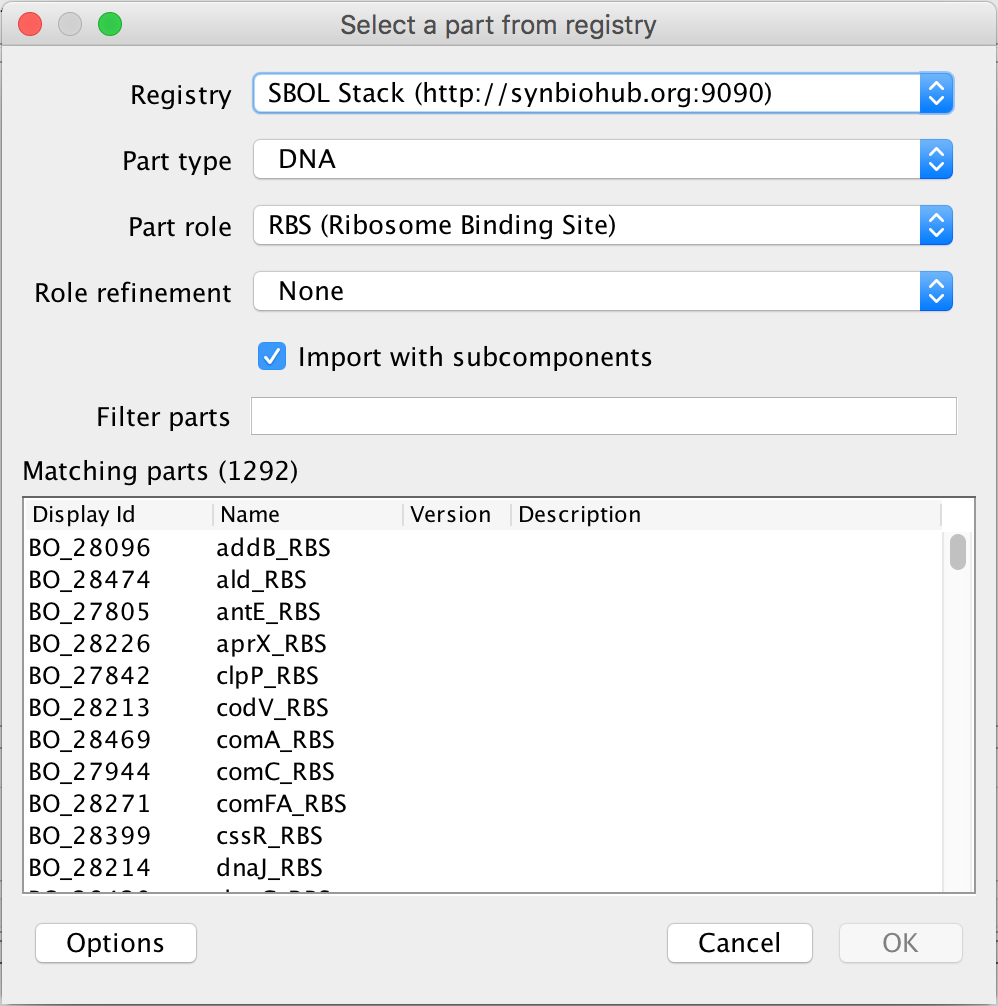
\includegraphics[width=110mm]{screenshots/PartPartRegistry}
\end{center}

\item The next step is to associate the ribosome binding site with its gene sequence, so in the Filter Parts criterion, type J61120. The filter is case sensitive so be sure to use a capital "J". The only DNA sequence left after the filter is the DNA sequence for this ribosome binding site, so select it and click Ok to associate it with this ribosome binding site. 

\begin{center}
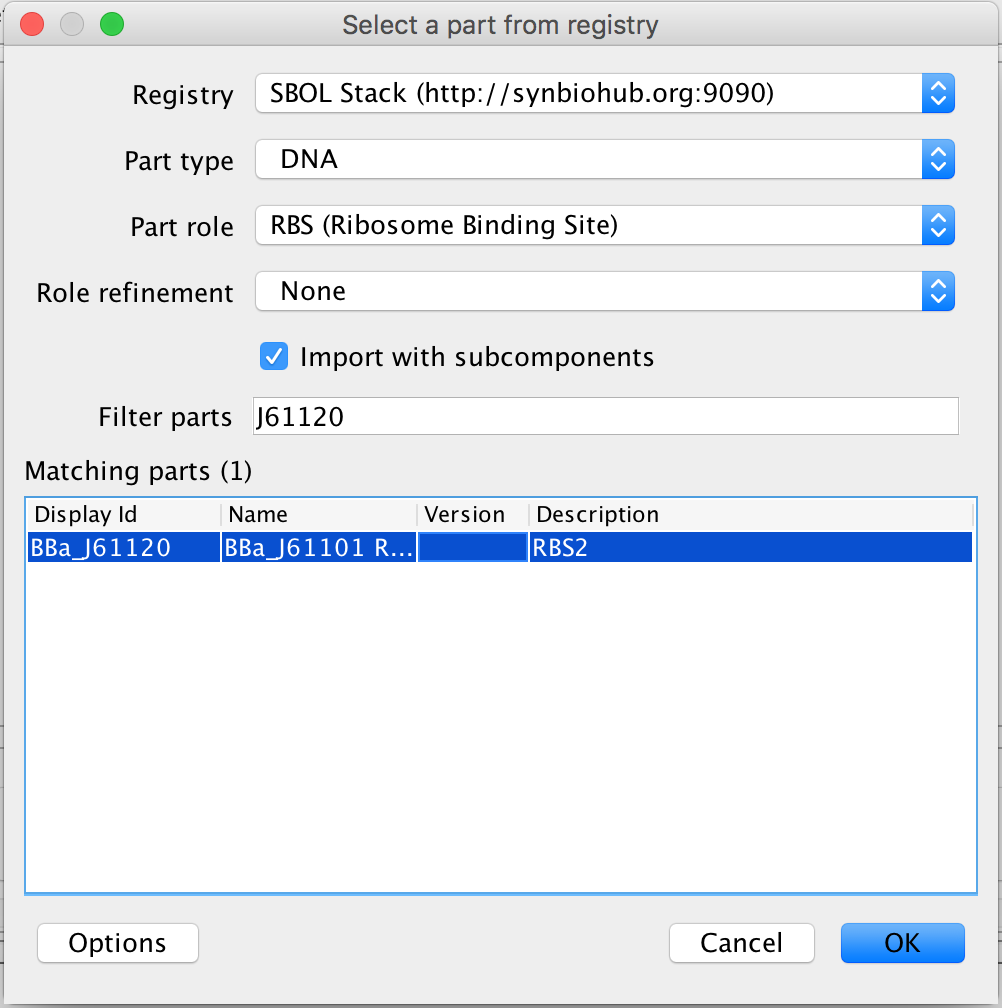
\includegraphics[width=110mm]{screenshots/PartRBSTetR}
\end{center}

\item Now that the ribosome binding site now has its DNA sequence associated with it, the same must now be done for the actual coding sequence for the TetR protein, so select the coding sequence and press the search part registry icon. Currently, the Part Registry takes a little longer to open for coding sequences than it does for ribosome binding sites, so be patient. When the Part Registry loads, enter in C0040 in the filter parts criterion, and select the tetR coding sequence and click Ok to associate it with the coding sequence.

\begin{center}
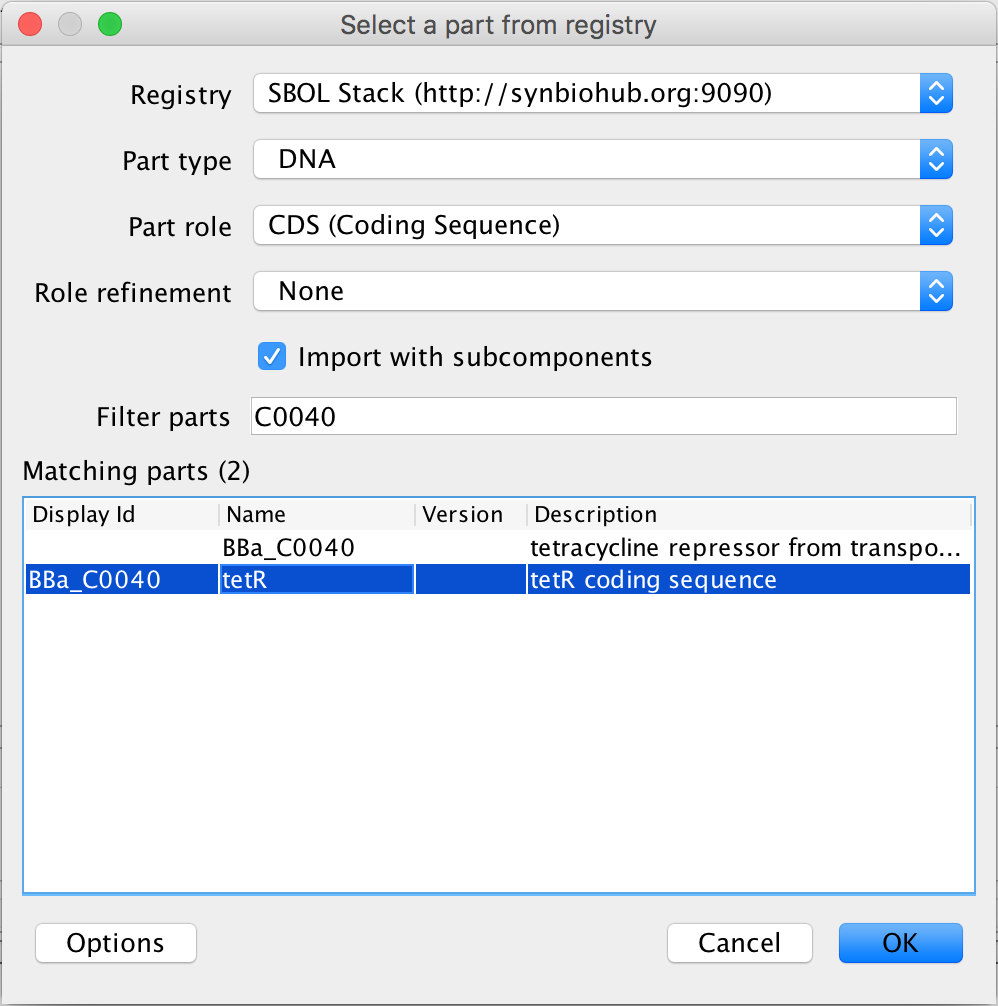
\includegraphics[width=110mm]{screenshots/PartCDSTetR}
\end{center}

\item Now that the TetR gene is associated with its DNA sequences, the next step is to focus out back to the genetic circuit as a whole and do the same for the GFP gene, so select the focus out icon. The focus out icon is the third icon from the right on the tool ribbon.

\begin{center}
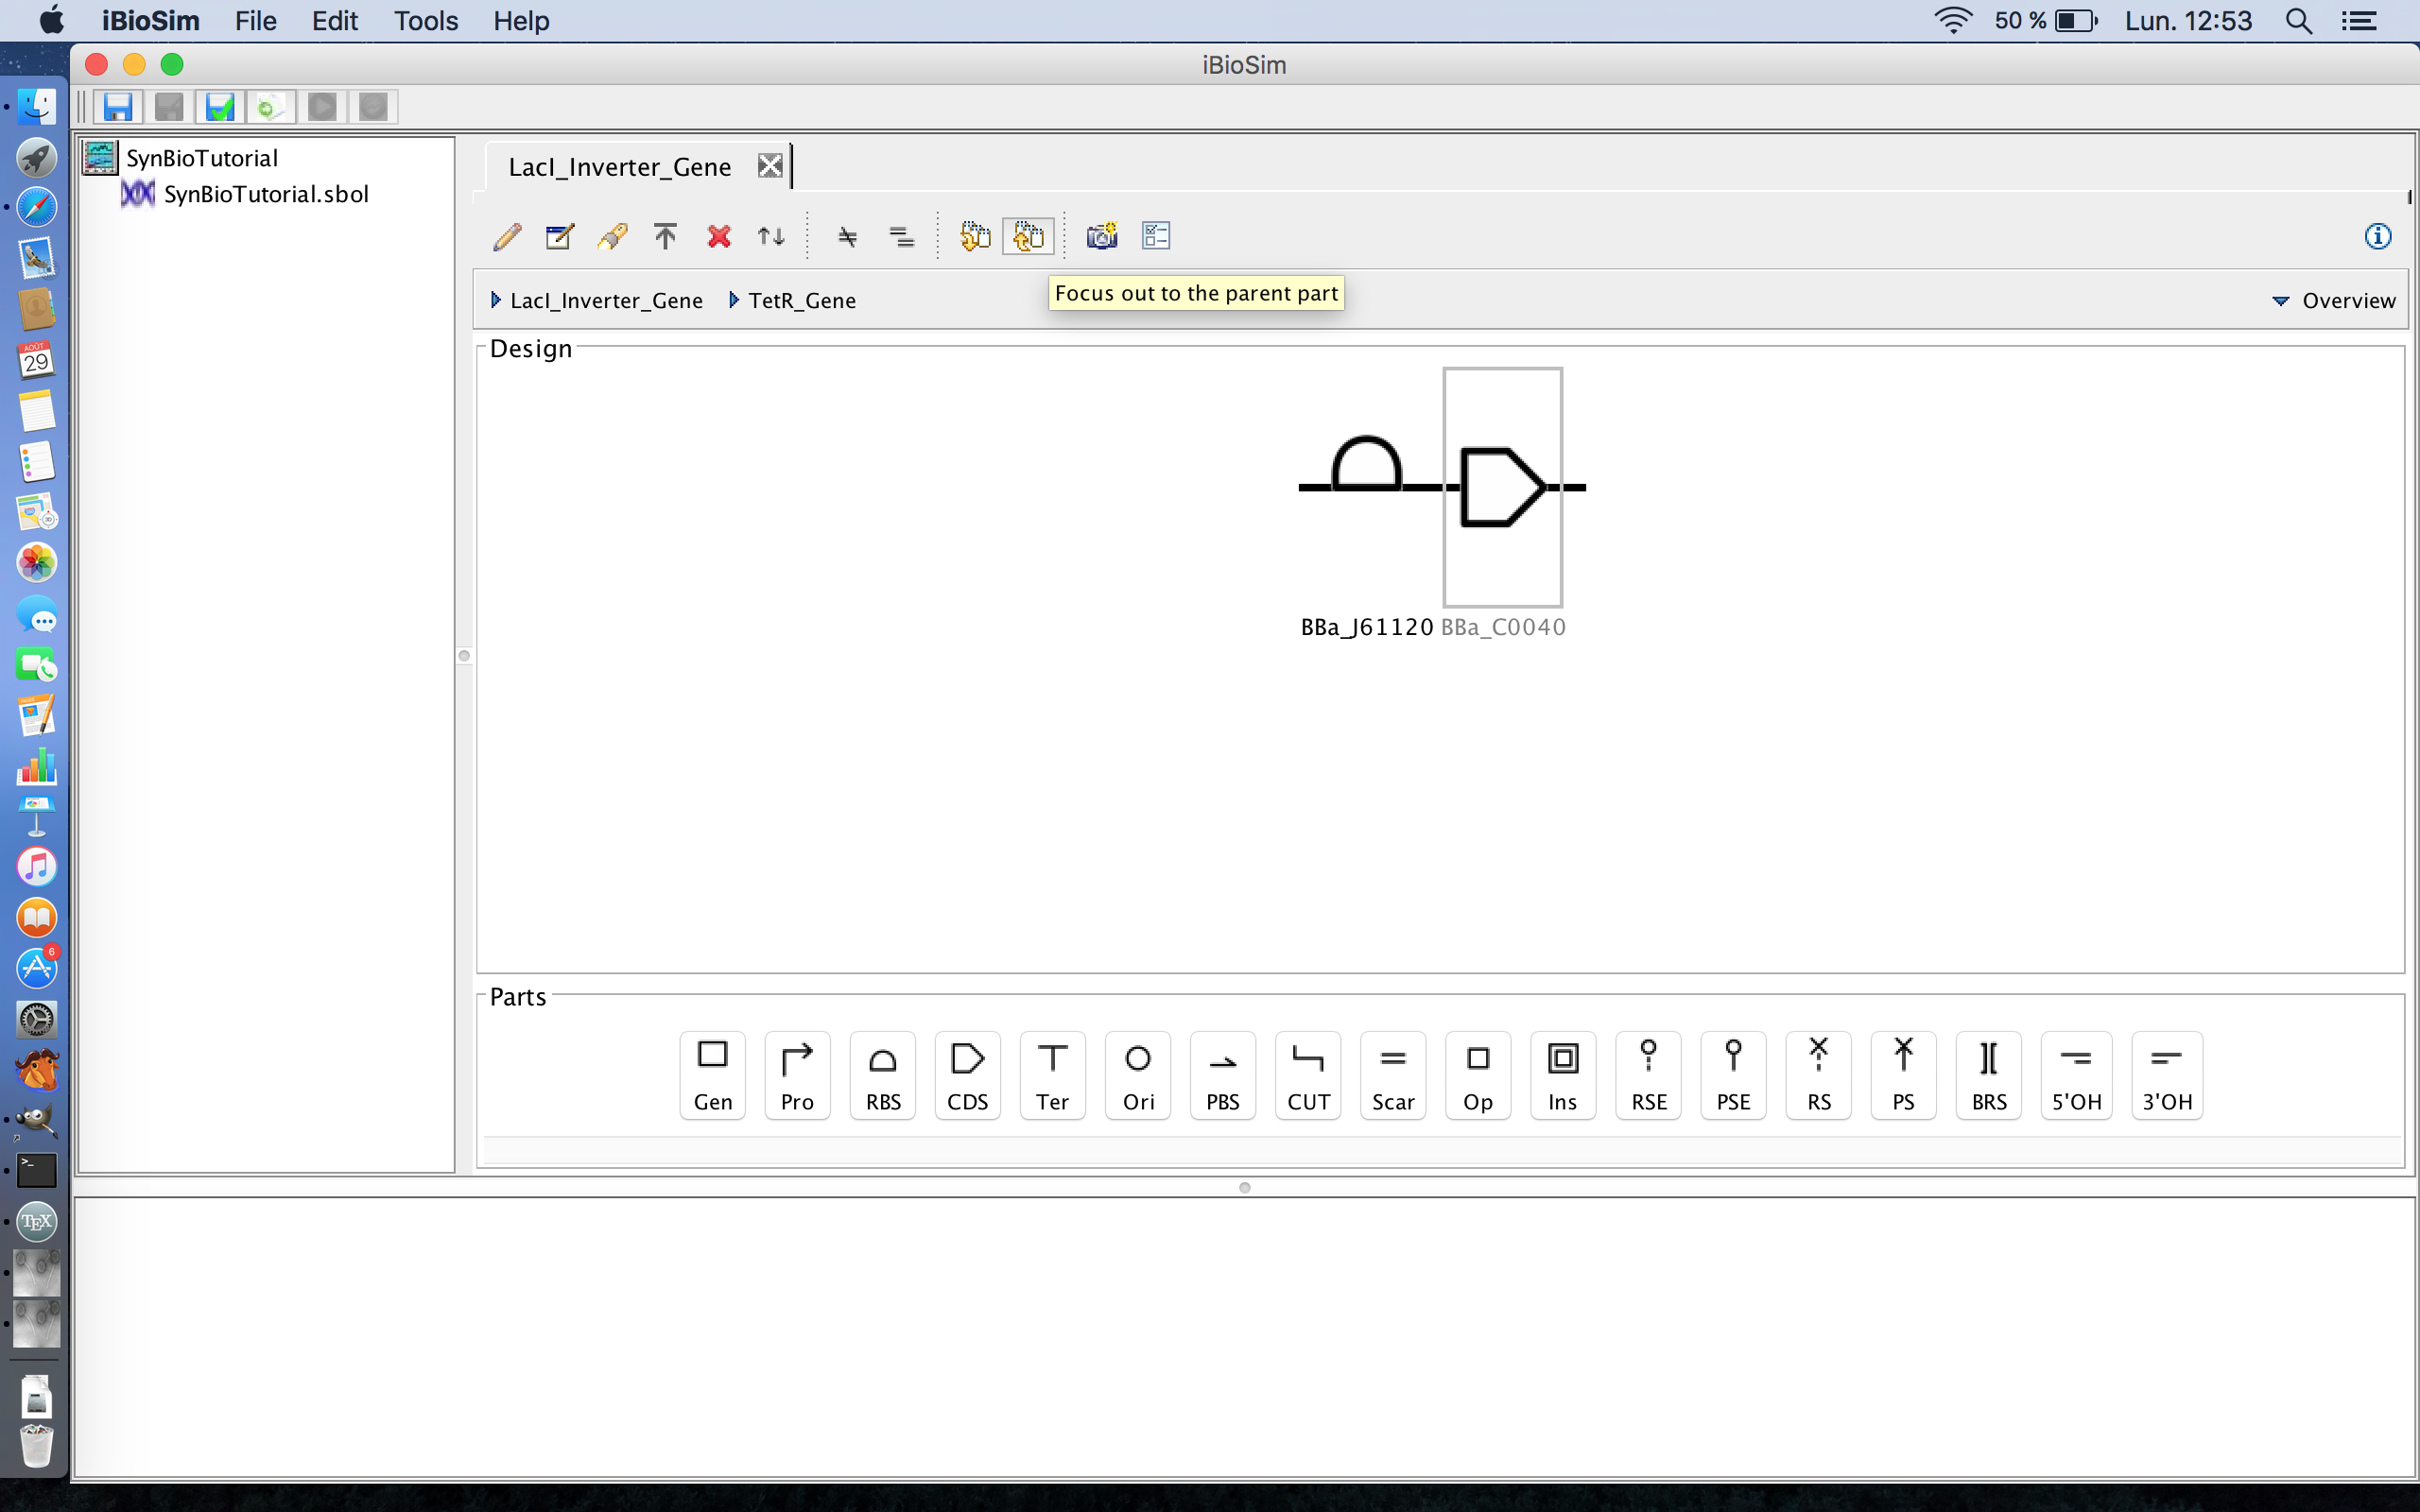
\includegraphics[width=160mm]{screenshots/PartFocusOut}
\end{center}

\item Now select the GFP gene and the focus in icon, and build that gene with a ribosome binding site and a coding sequence.

\begin{center}
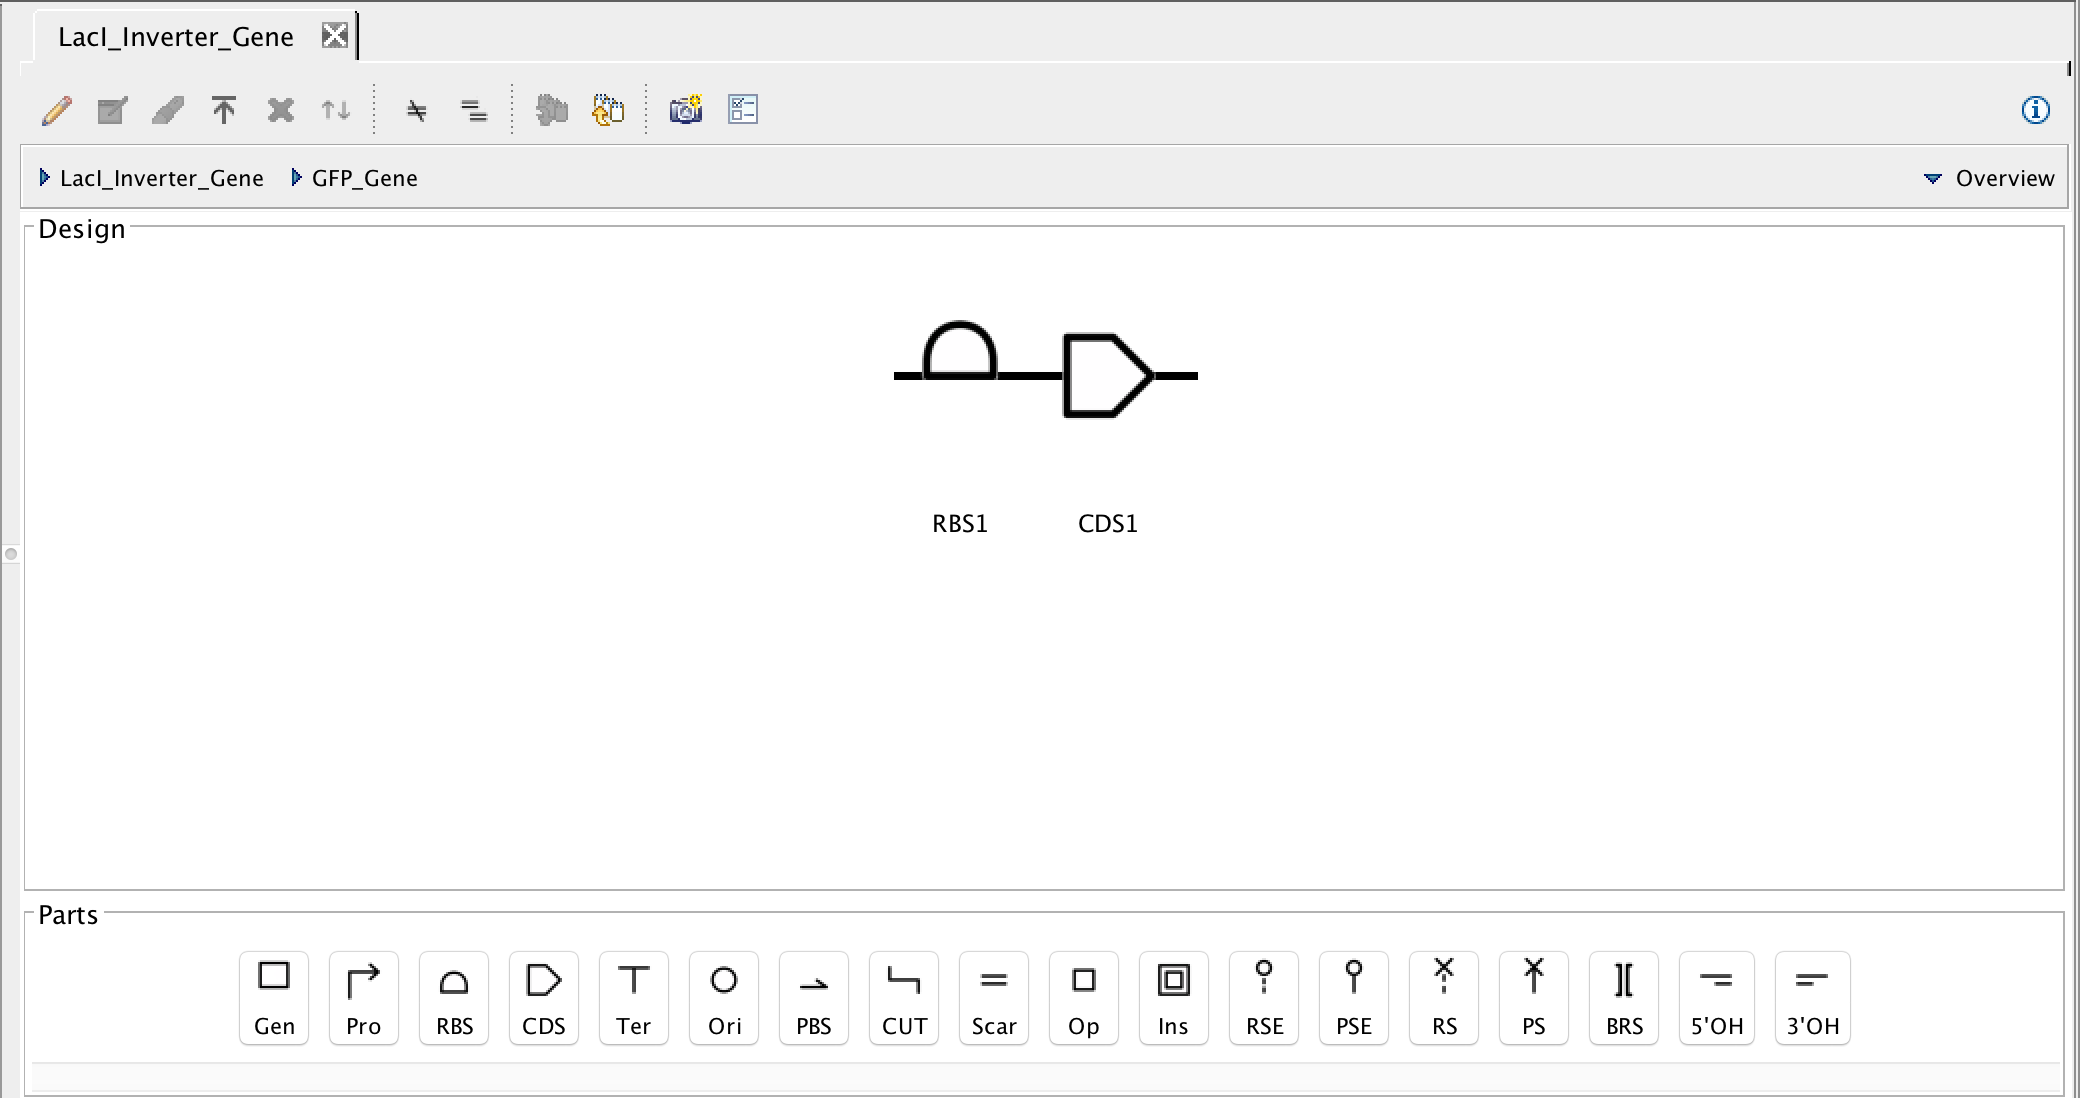
\includegraphics[width=160mm]{screenshots/PartGFPFocusIn}
\end{center}

\item Like before, the next step is to associate the ribosome binding site and the coding sequence with their respective DNA sequences, so select the ribosome binding site and the search part registry icon. In the filter criterion, type J61130, and the select the DNA sequence and associate it with the ribosome binding site by pressing Ok.

\begin{center}
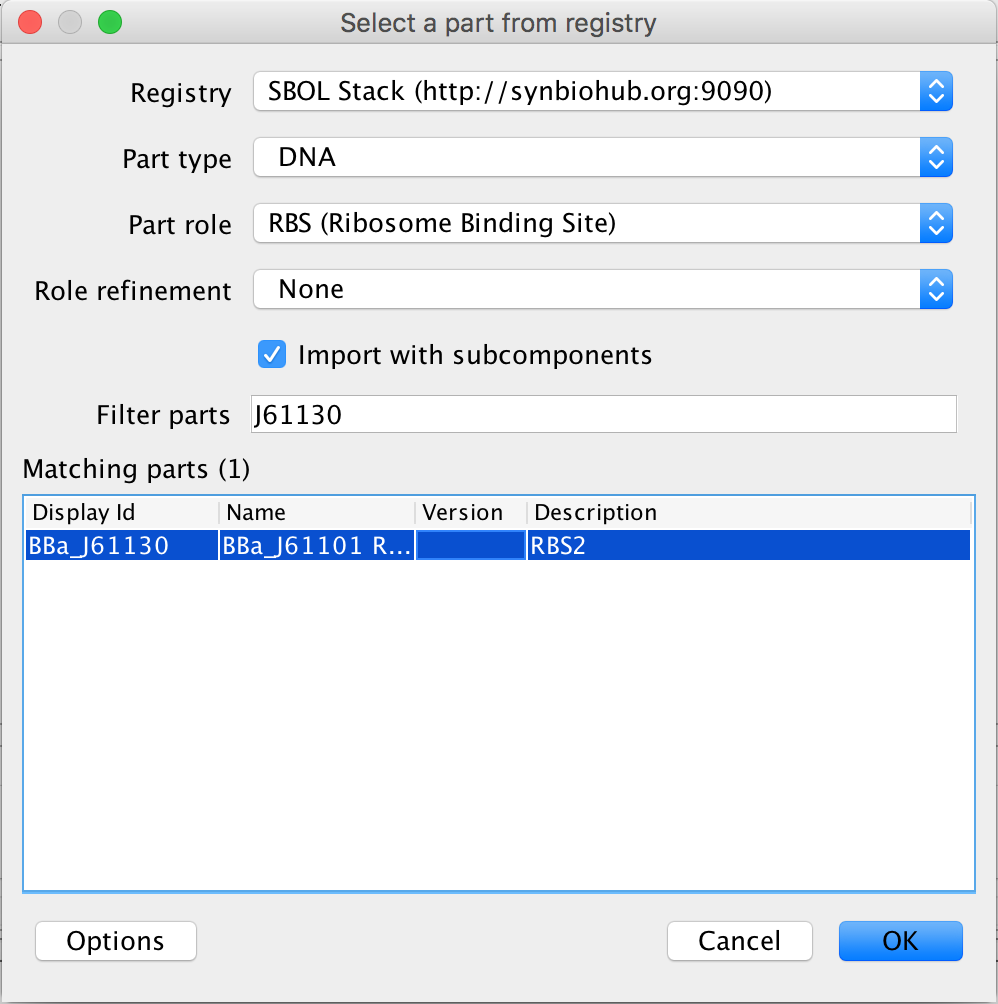
\includegraphics[width=110mm]{screenshots/PartRBSGFP}
\end{center}

\item Next, select the coding sequence and the search part registry icon and type E0040 into the filter criterion and select the gfp coding sequence. Then, press Ok.

\begin{center}
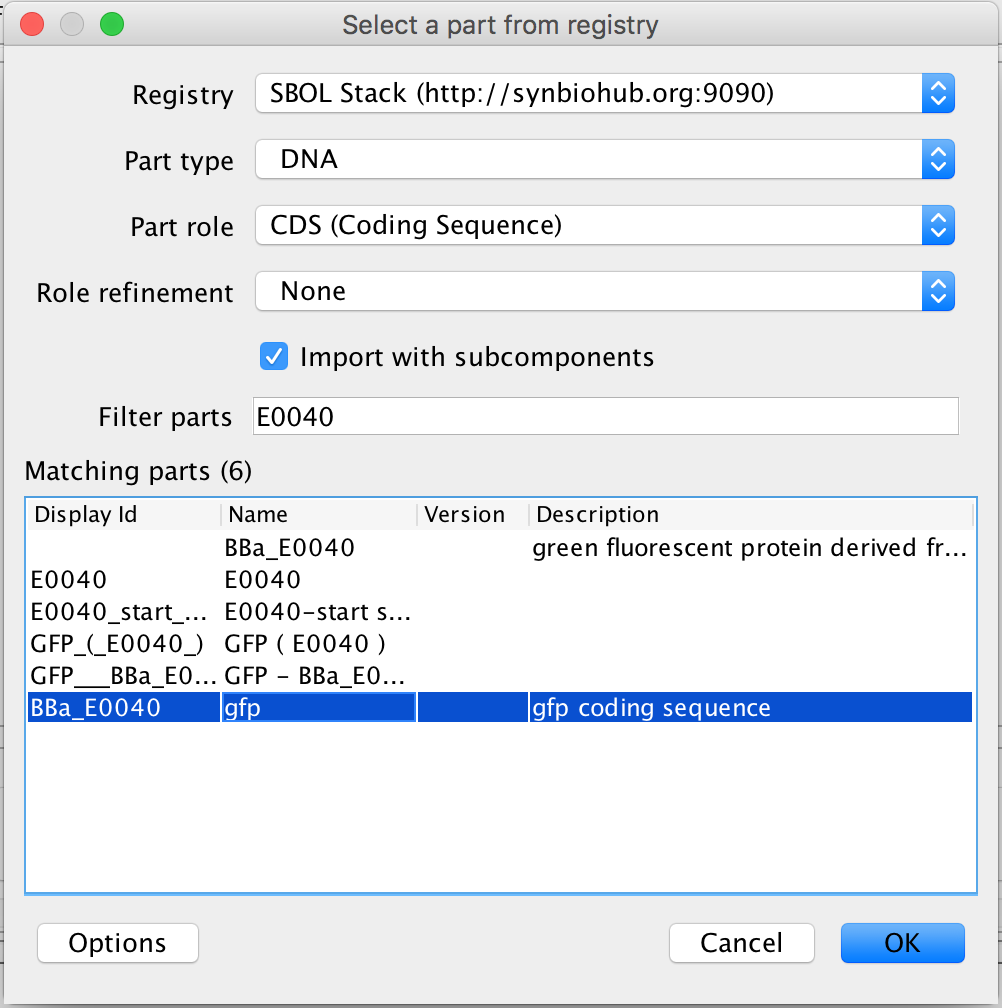
\includegraphics[width=110mm]{screenshots/PartCDSGFP}
\end{center}

\begin{center}
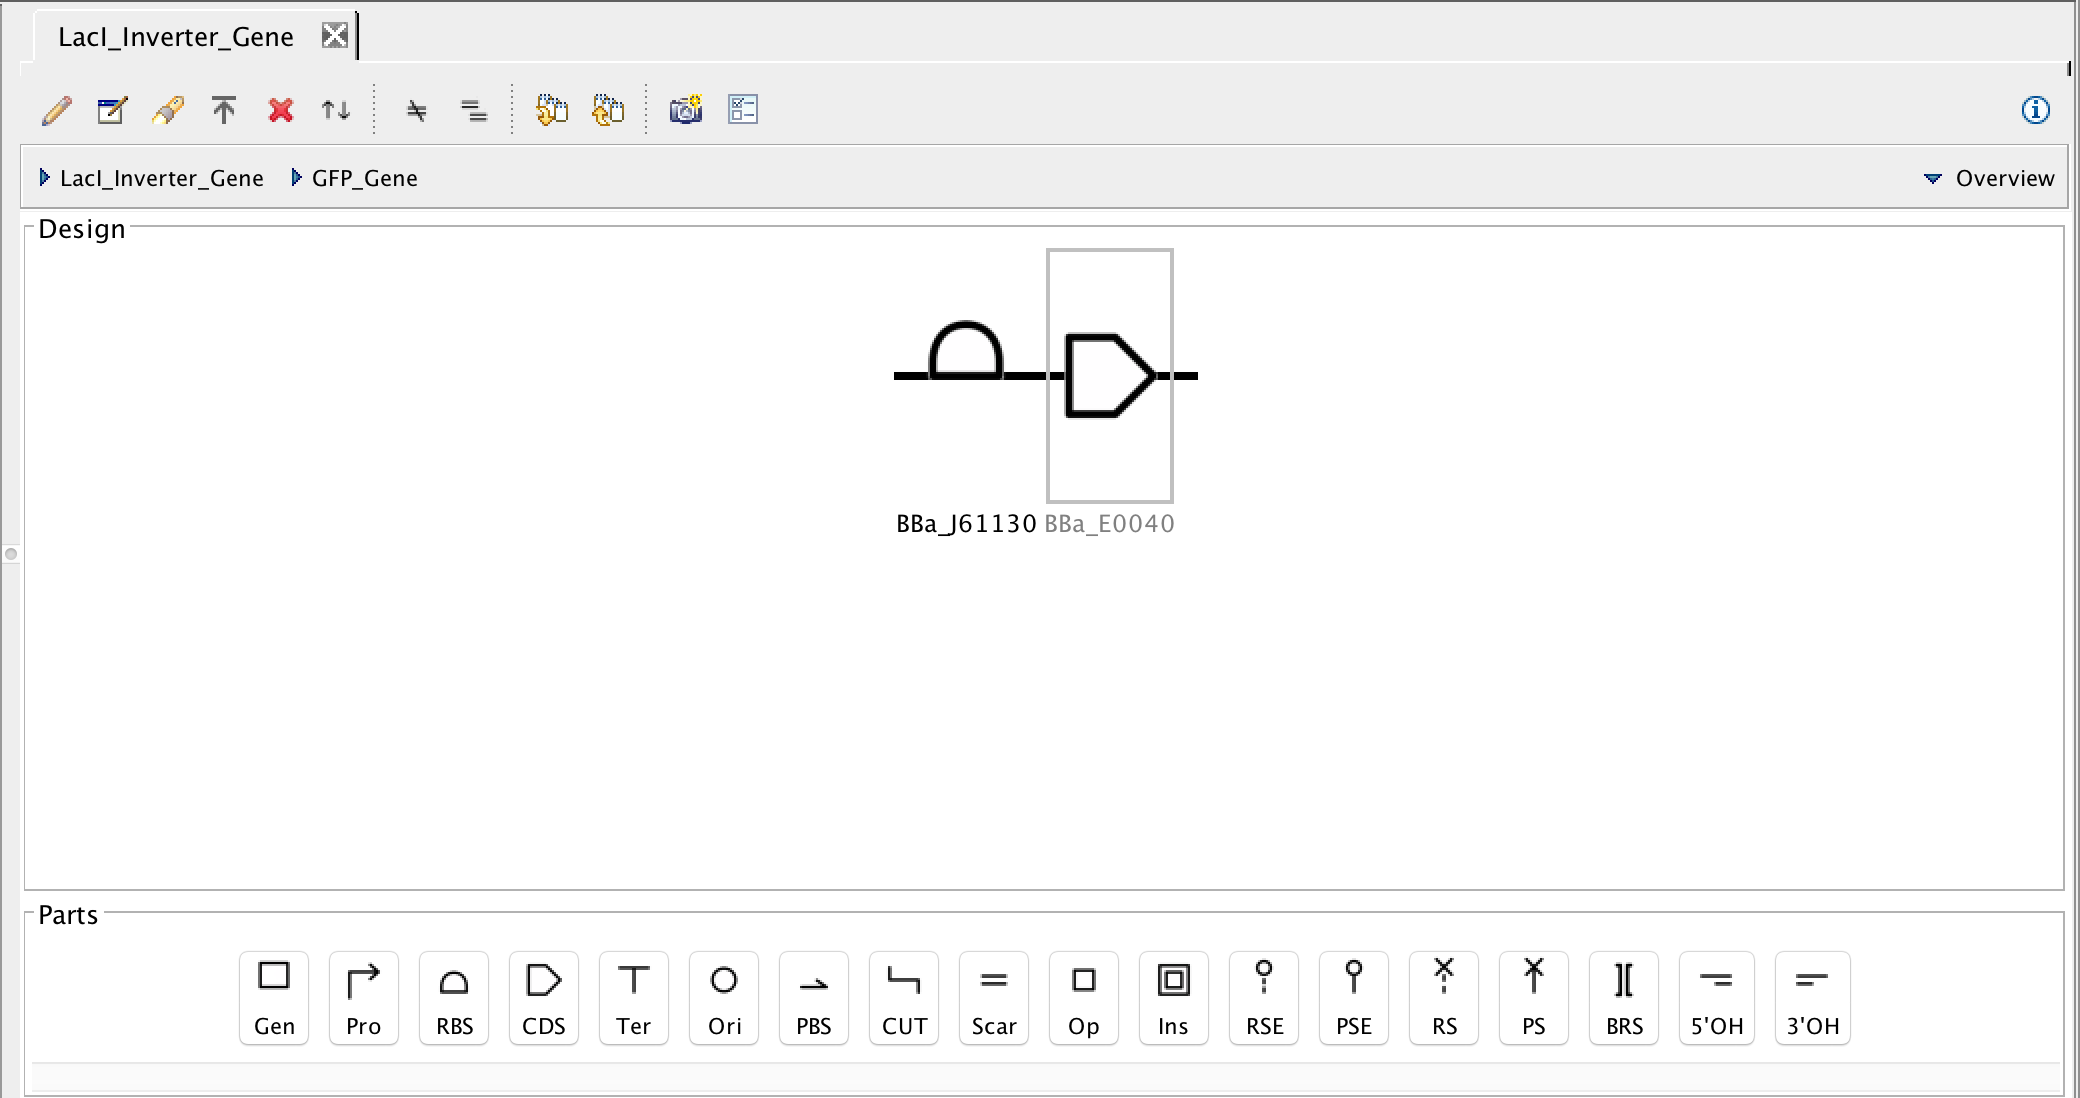
\includegraphics[width=160mm]{screenshots/PartGFPGeneComplete}
\end{center}

\item Now that the GFP gene is complete, focus back out to the genetic circuit as a whole to associate the promoter and terminator with their DNA sequences. Next, select the promoter and the search part registry icon. Then type R0010 in the filter criterion and select the pLac promoter and press Ok.

\begin{center}
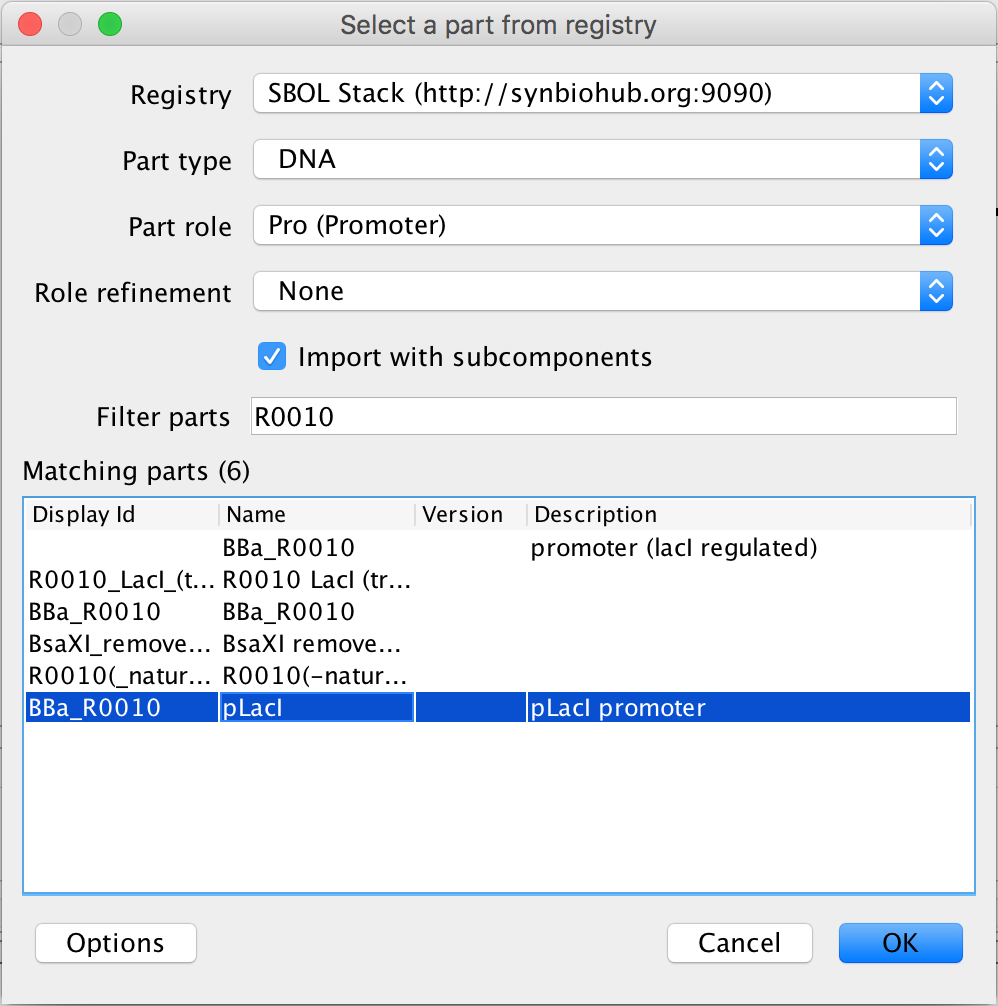
\includegraphics[width=110mm]{screenshots/PartLacIPromoter}
\end{center}

\item Now select the terminator and the search part registry icon. This time, type ECK to narrow the selection to two terminators, and select terminator 2. Then, press Ok.

\begin{center}
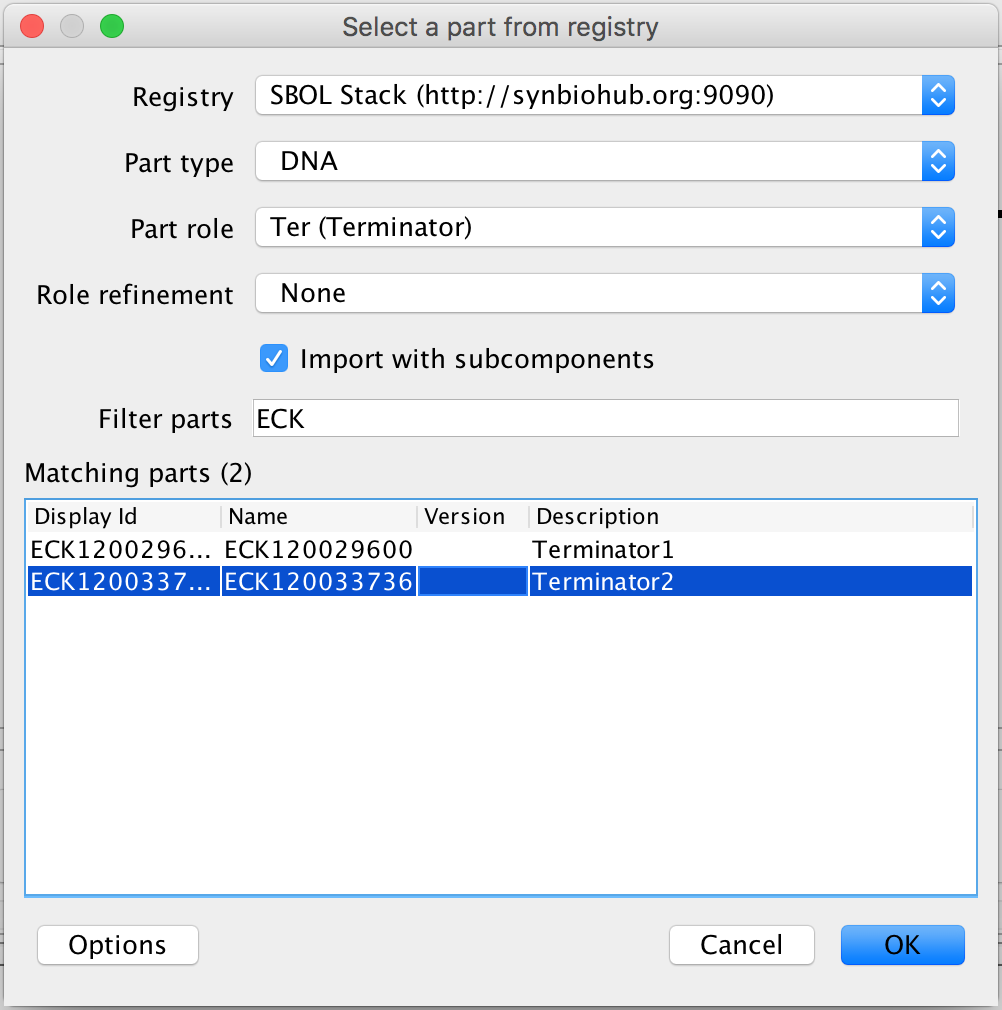
\includegraphics[width=110mm]{screenshots/PartLacIComplete}
\end{center}

\item Now that this genetic circuit is complete, in order to successfully integrate it later in the model, it must be saved before continuing. This can be done by selecting the file menu and clicking save or by using the shortcut control $\rightarrow$ S on the Windows and Linux versions or command $\rightarrow$ S on the Mac OS version. You will then be prompted that you are saving into an existing SBOL file. Currently, the part editor works by creating the SBOL when it is opened, so each time the file is saved, it appears to save onto an existing file, so ignore the message and select the Overwrite button.

\begin{center}
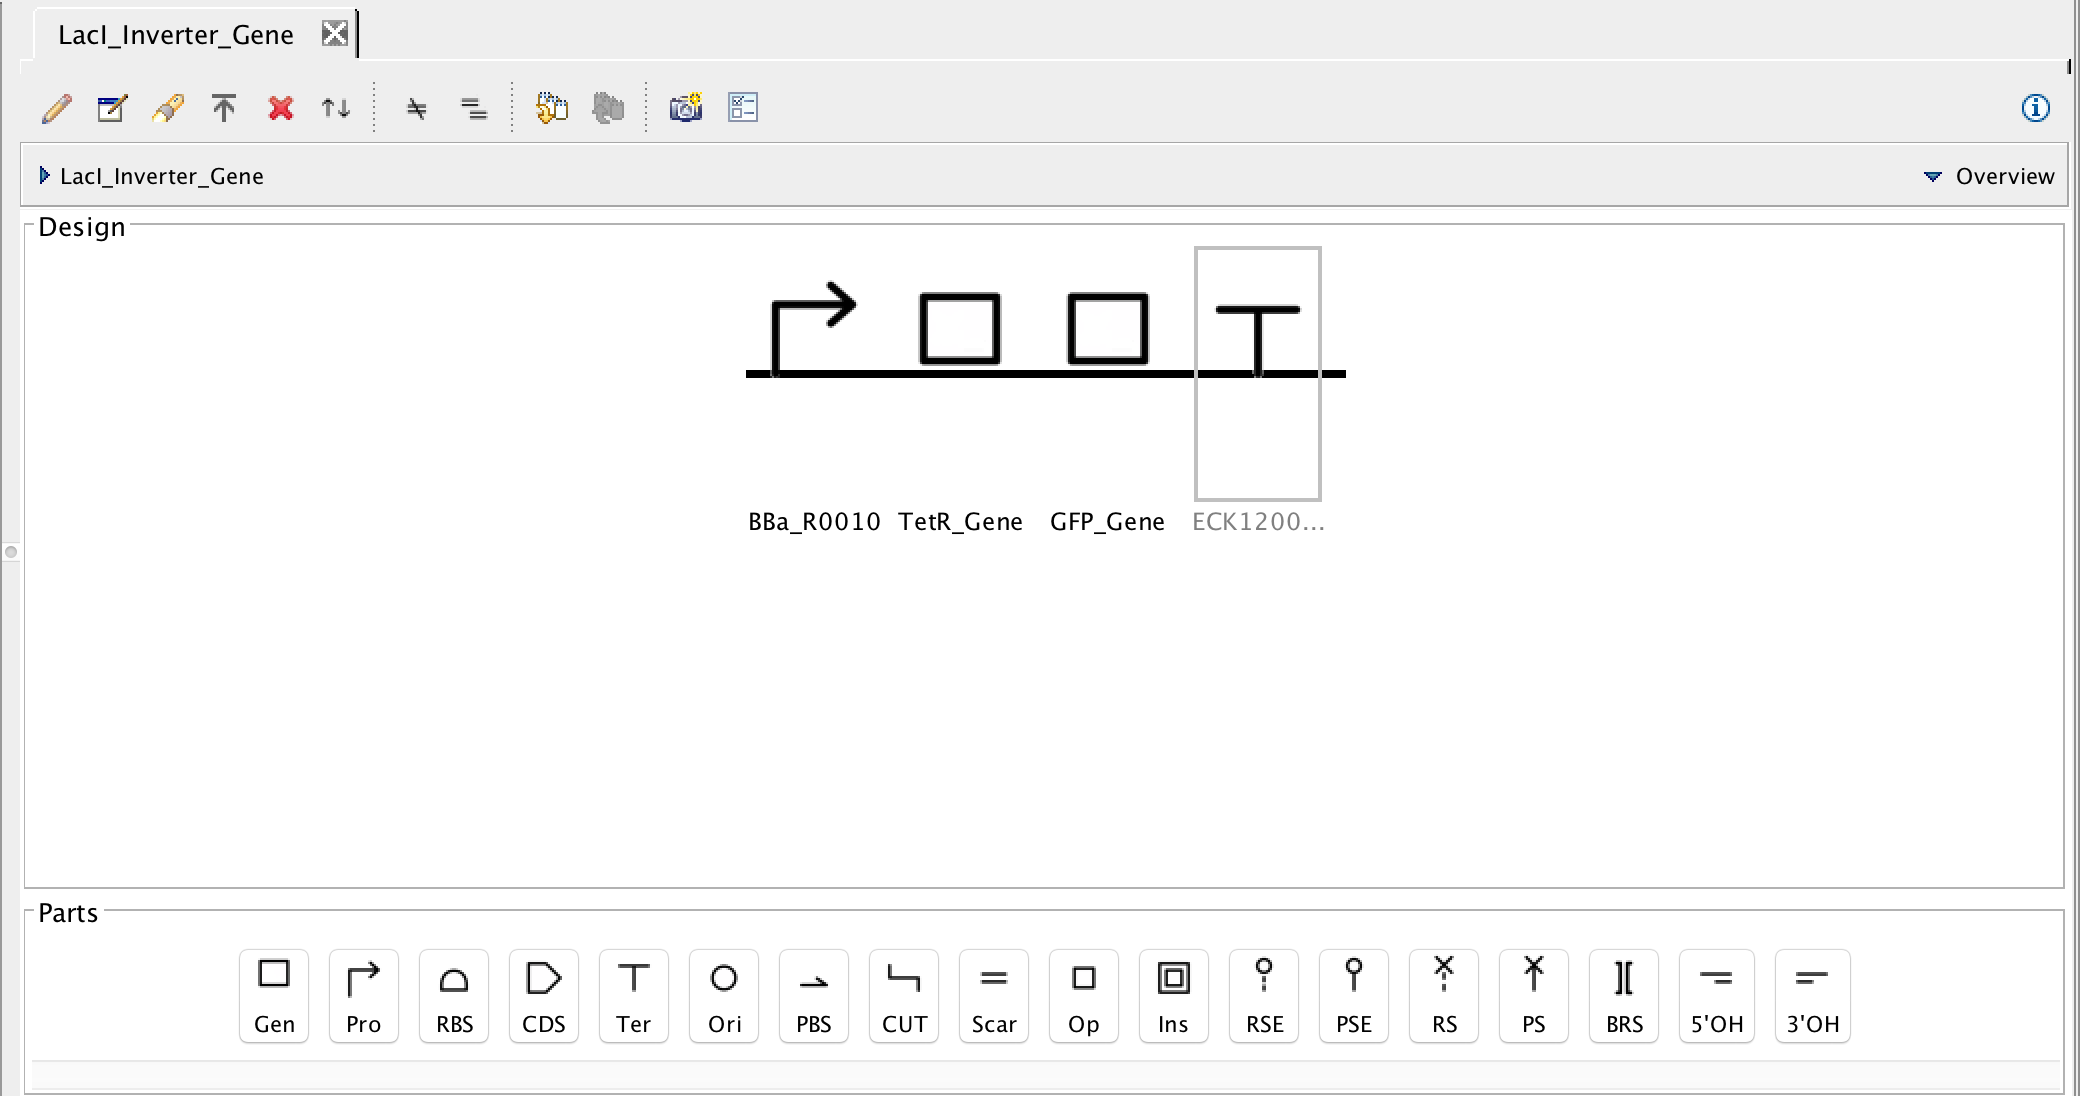
\includegraphics[width=160mm]{screenshots/PartLacIComplete2}
\end{center}

\begin{center}
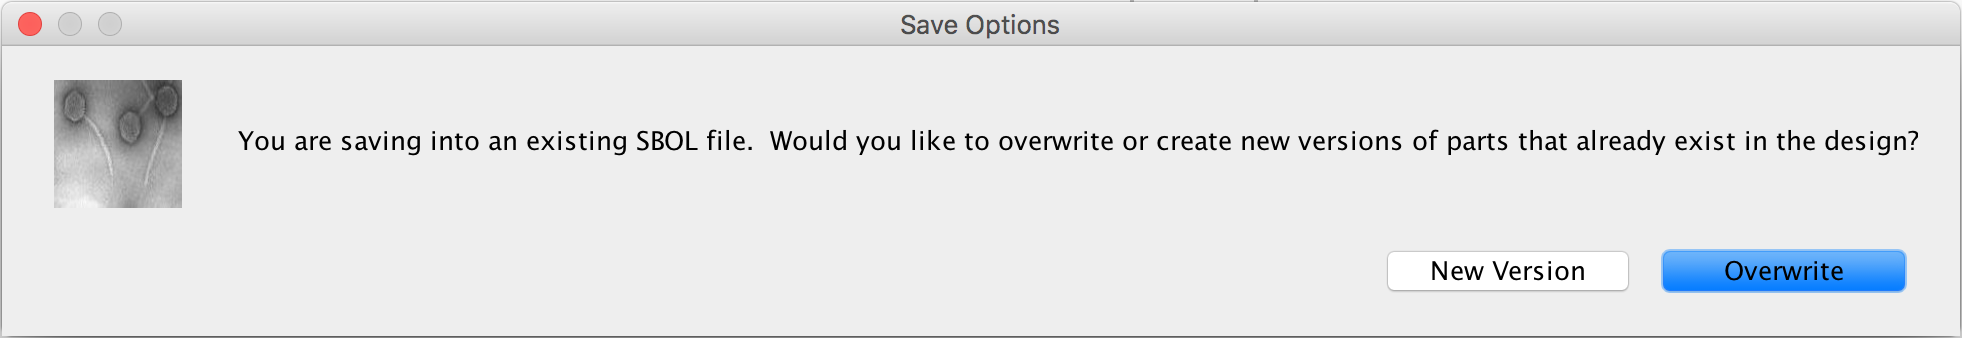
\includegraphics[width=160mm]{screenshots/PartSave}
\end{center}

\subsection{TetR Inverter Gene}
\item As aforementioned, there are two genetic circuits in this model, so now it is time to create the next one. Select the file menu, hover over New, and select Part. You will then be prompted to enter a Part ID, so enter TetR\_Inverter\_Gene.

\begin{center}
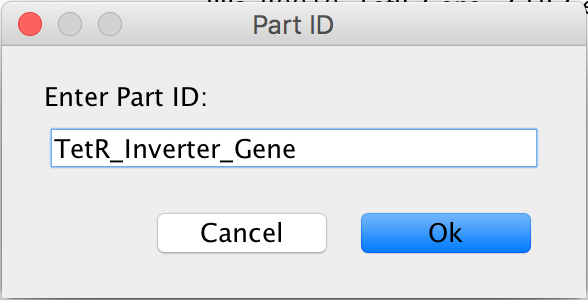
\includegraphics[width=75mm]{screenshots/PartIDTetR}
\end{center}

\item The next steps are more or less the same as the LacI Inverter genetic circuit. The difference in this circuit is that there is only one gene, so insert a promoter, and then a gene. In the Gene Editor, under the Display ID criterion, enter LacI because this is the gene that codes for the LacI repressor protein in the previous genetic circuit.

\begin{center}
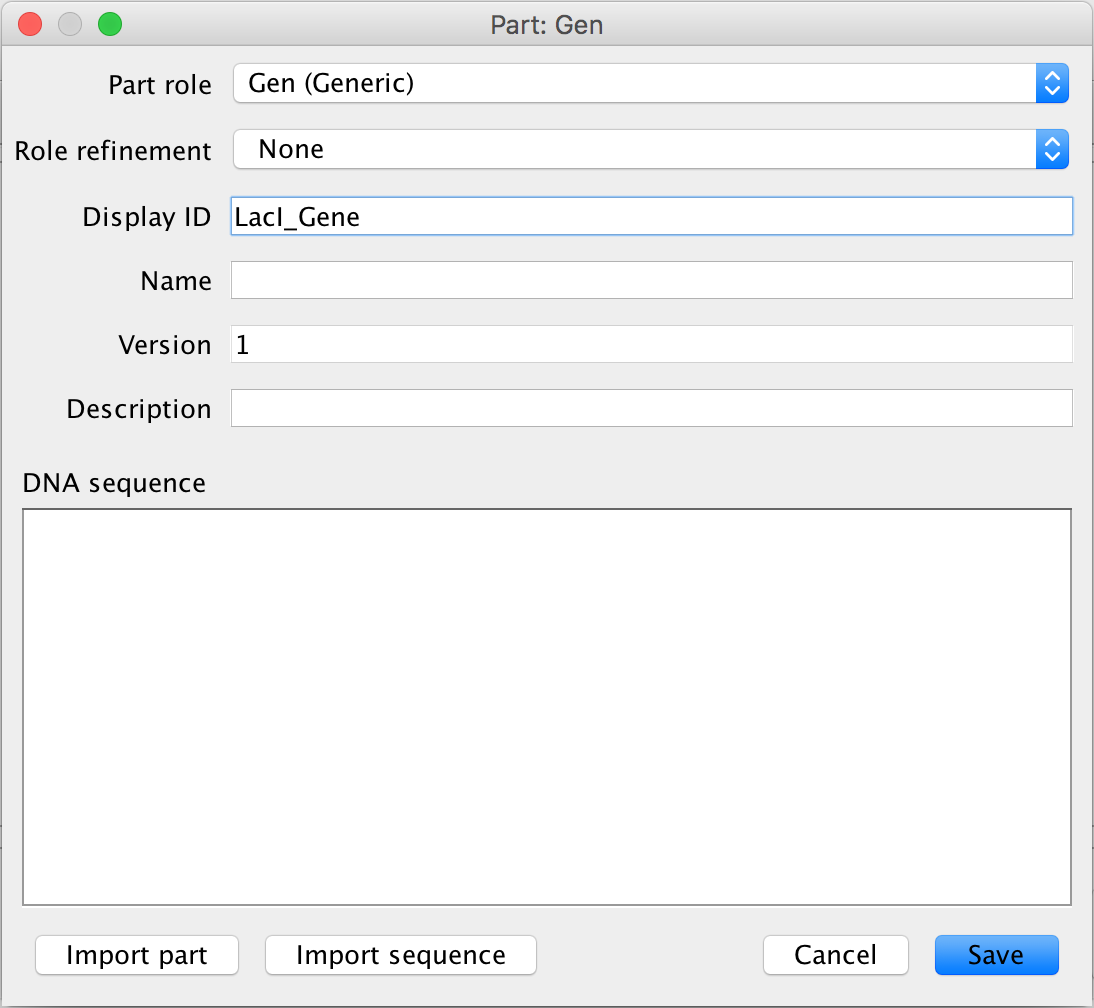
\includegraphics[width=110mm]{screenshots/PartLacIGene}
\end{center}

\item Next, as before, insert the terminator. Then focus in to the LacI gene and insert a ribosome binding site and coding sequence as before.

\begin{center}
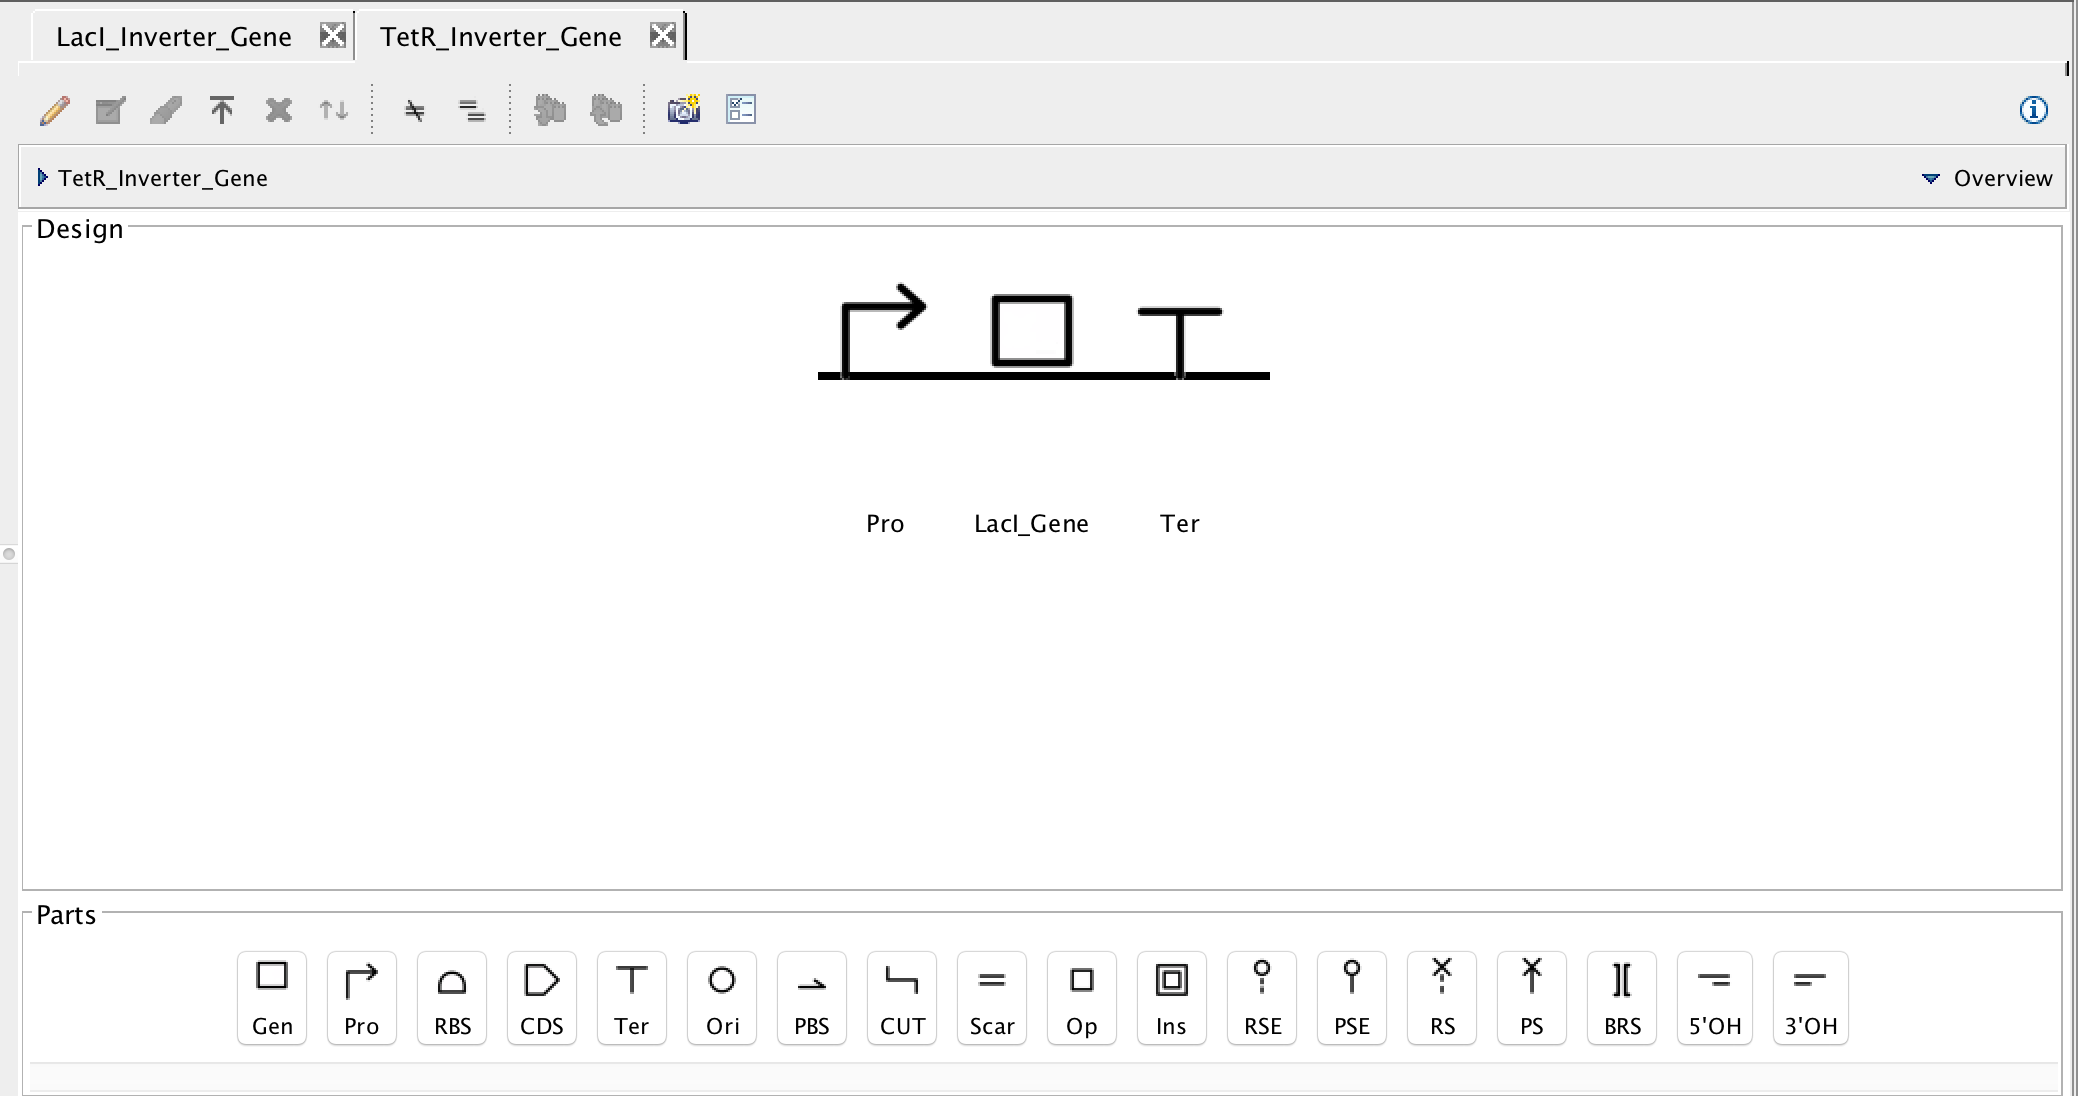
\includegraphics[width=160mm]{screenshots/PartTetRAssembled}
\end{center}

\begin{center}
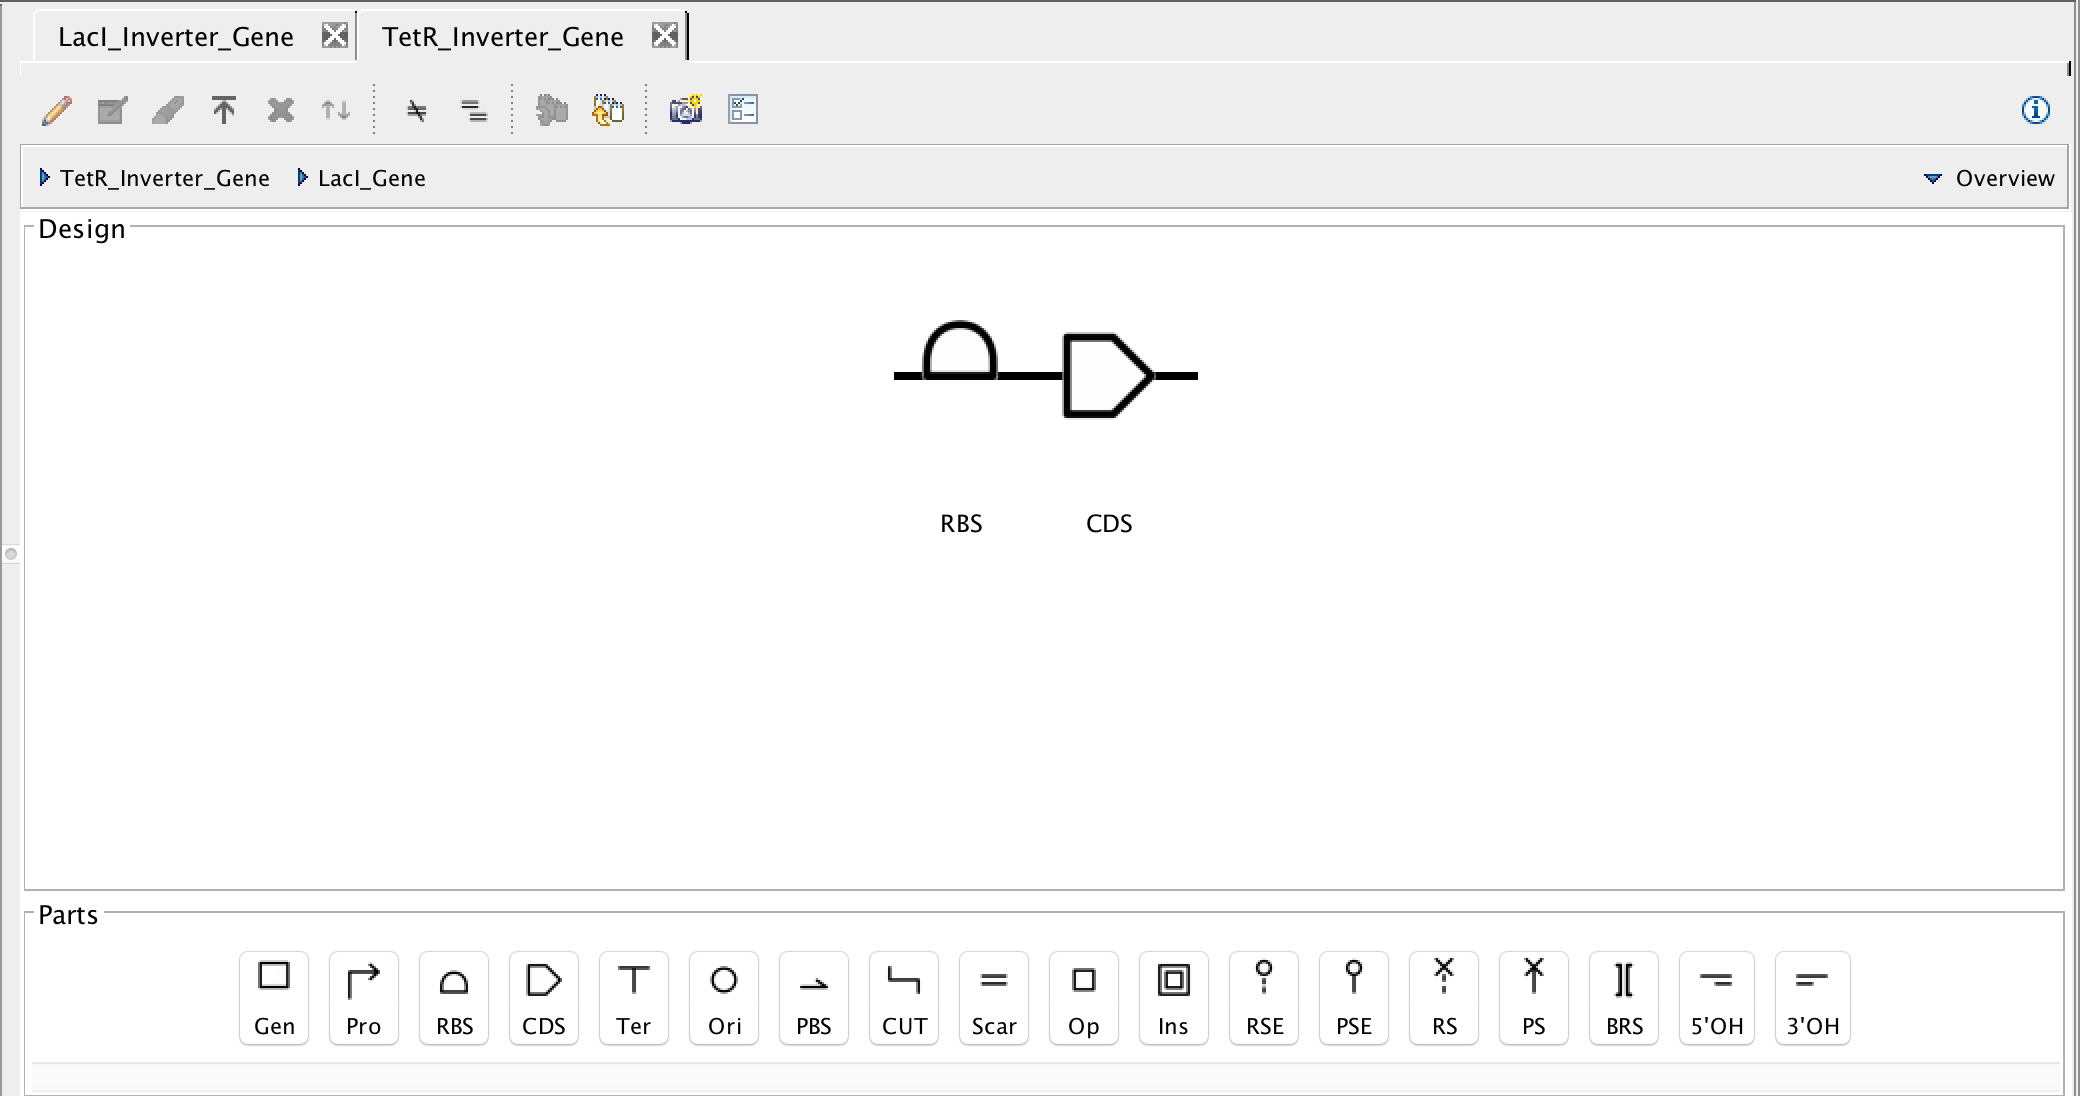
\includegraphics[width=160mm]{screenshots/PartTetRLacIAssembled}
\end{center}

\item Now, it is once again time to associate each part of the circuit with its DNA sequence, so select the ribosome binding site and the search part registry icon. In the filter parts criterion, type J61101, and select the one that has J61101 in the Display Id and press Ok.

\begin{center}
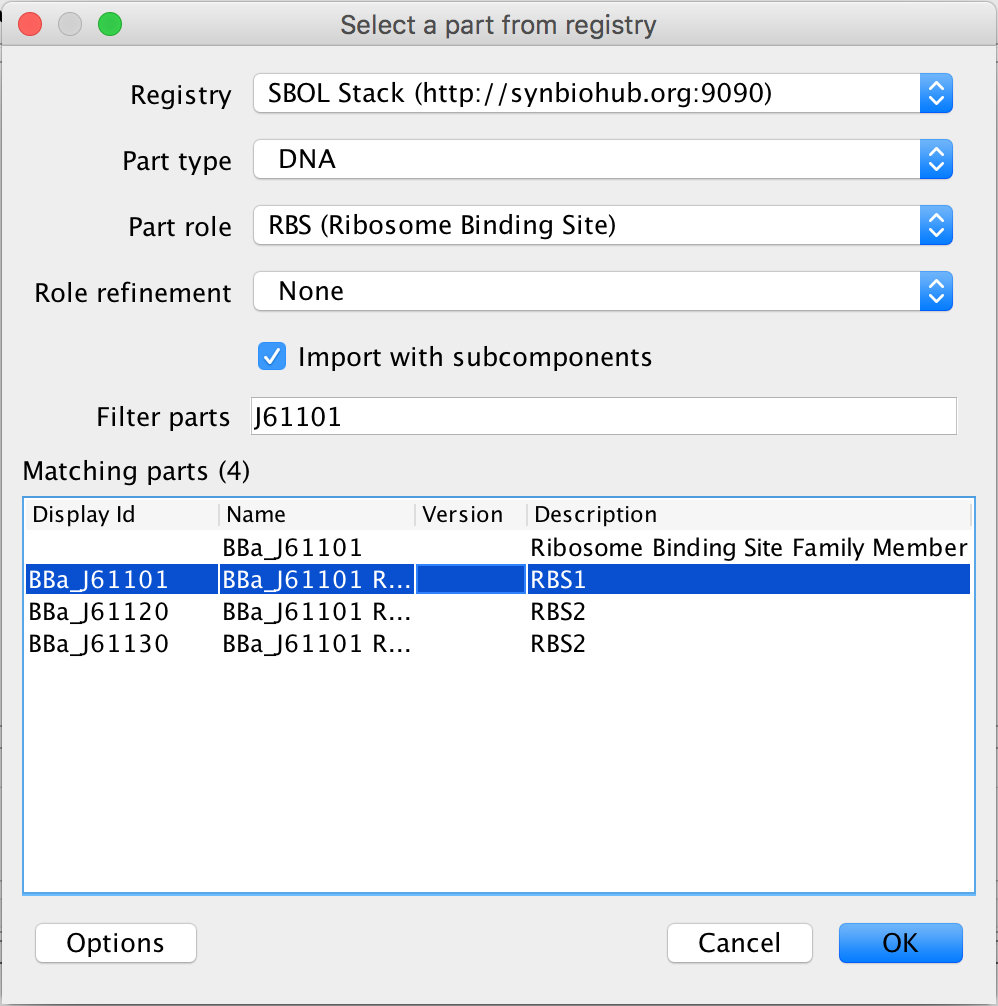
\includegraphics[width=110mm]{screenshots/PartTetRRBS}
\end{center}

\item Next, select the coding sequence and the search part registry icon. This time in the filter parts criterion, type C0012 and select the lacI coding sequence and press Ok.

\begin{center}
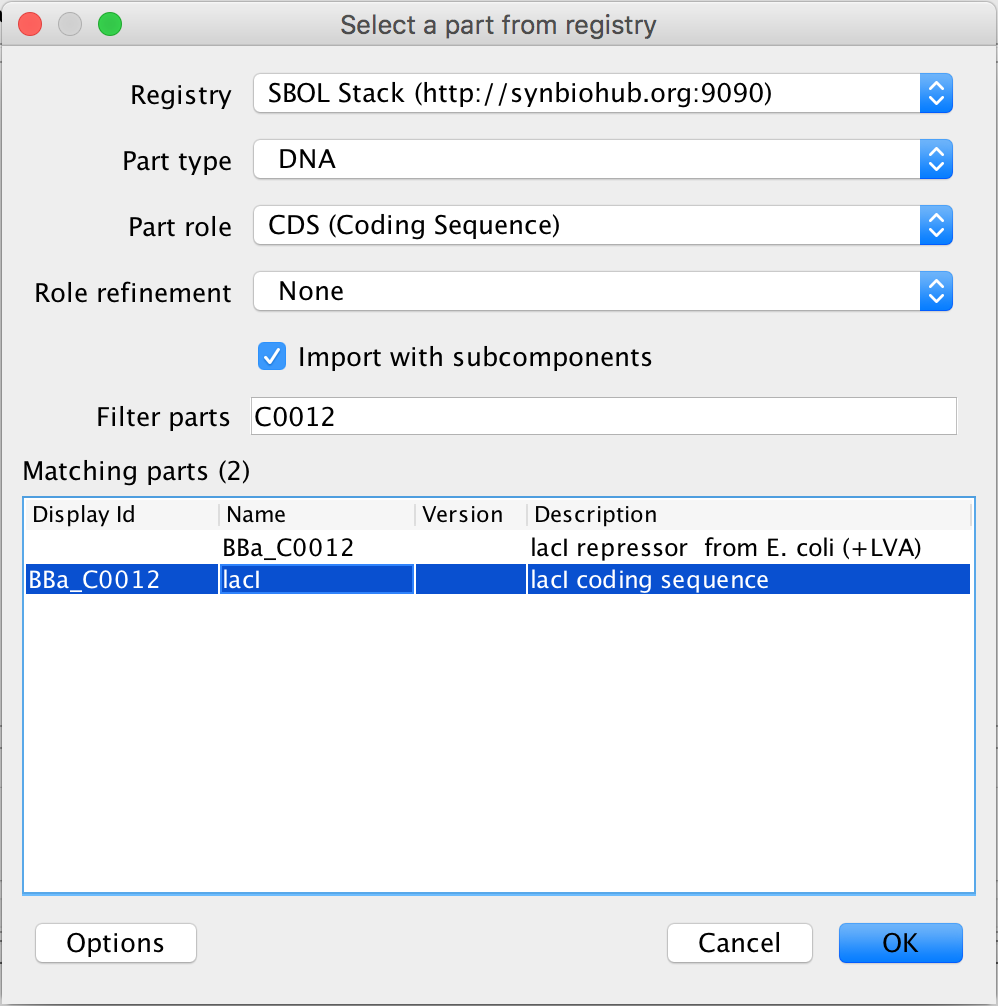
\includegraphics[width=110mm]{screenshots/PartLacICDS}
\end{center}

\begin{center}
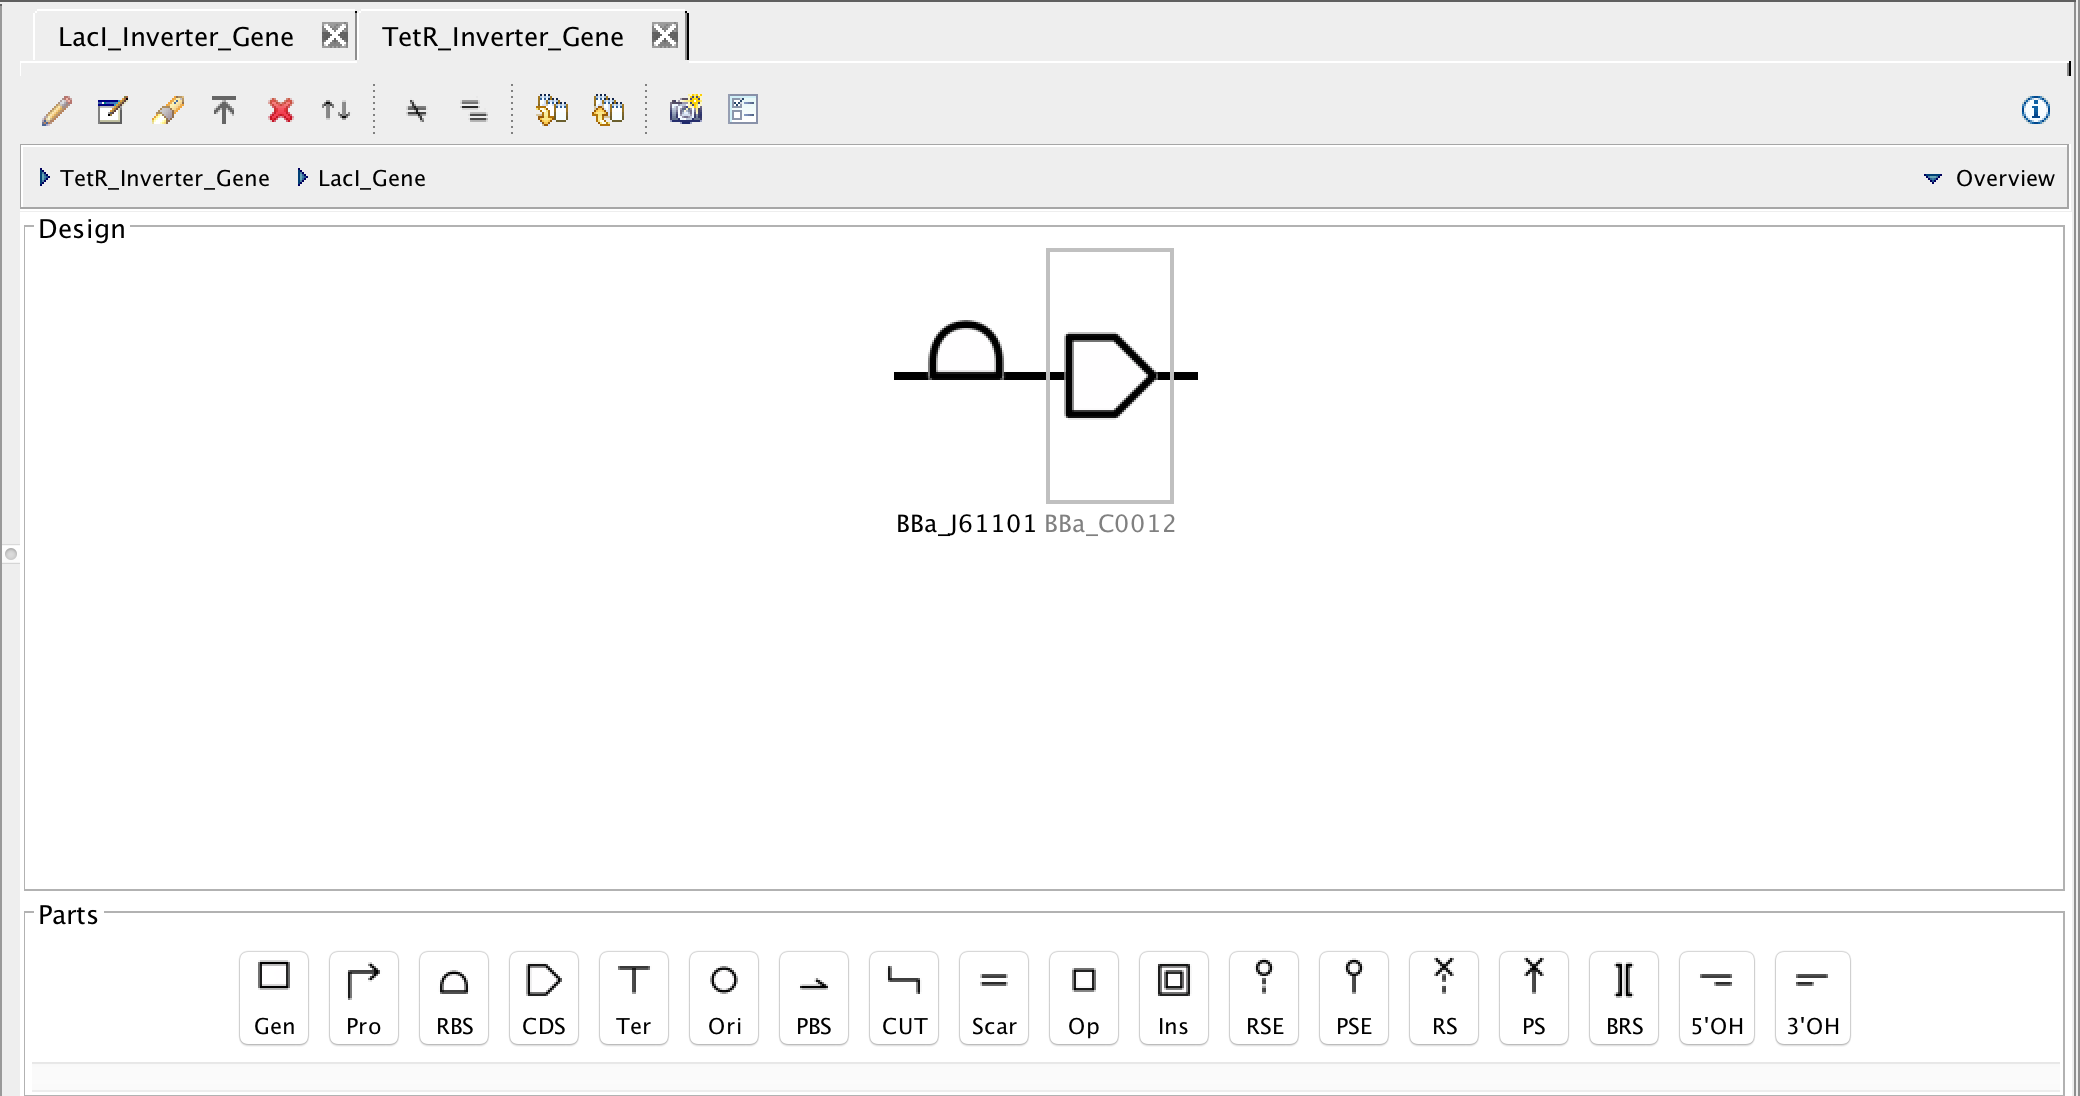
\includegraphics[width=160mm]{screenshots/PartLacIGeneComplete}
\end{center}

\item Next, as before, focus out. Now, it is time to associate the promoter and terminator with their DNA sequences, so select the promoter and the search part registry icon. Type R0040 into the filter parts criterion, and select the pTet promoter. Then associate the DNA sequence by pressing Ok.

\begin{center}
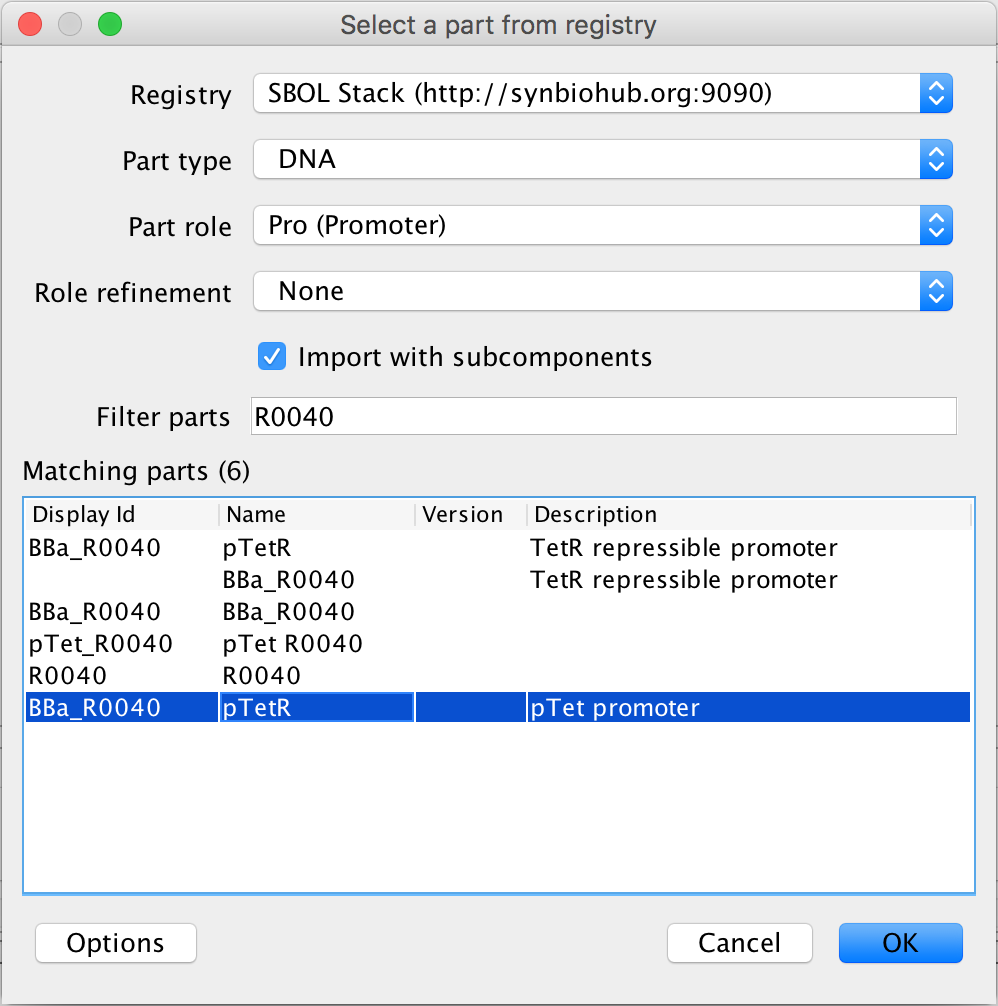
\includegraphics[width=110mm]{screenshots/PartpTetPromoter}
\end{center}

\item Now, to finish this genetic circuit, select the terminator and the search part registry icon in order to associate it to its DNA sequence. In the filter parts criterion, type ECK1200 and select Terminator 1 and press Ok to complete the genetic circuit.

\begin{center}
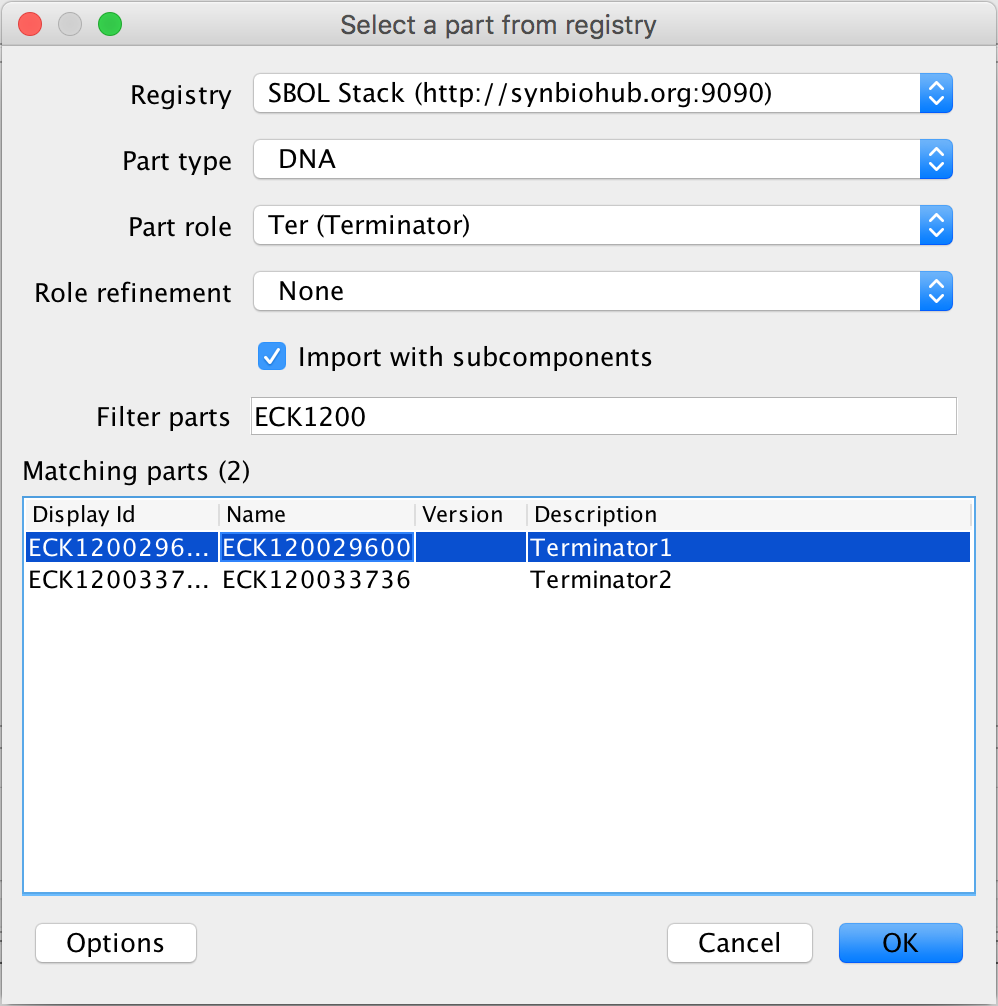
\includegraphics[width=110mm]{screenshots/PartTetRTerminator}
\end{center}

\begin{center}
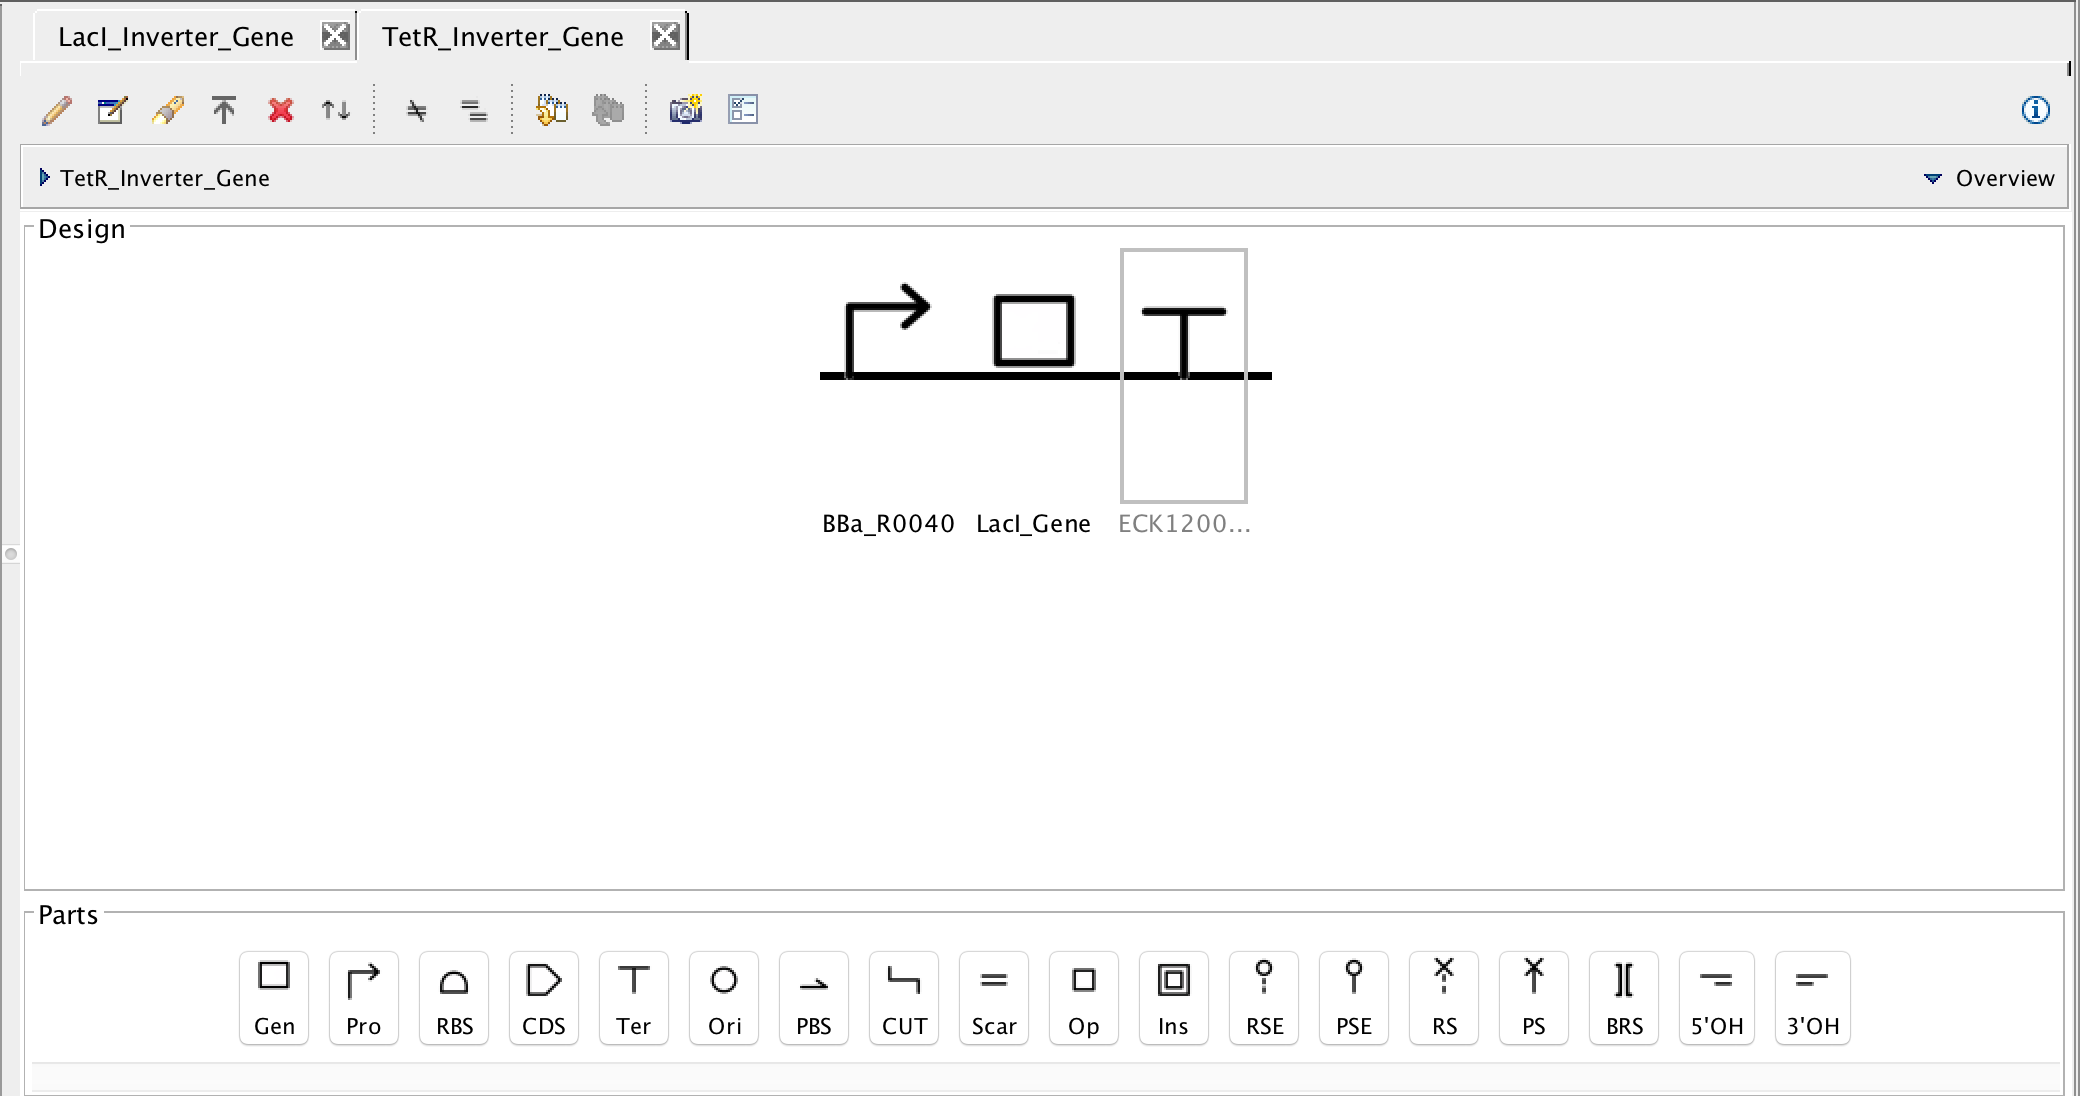
\includegraphics[width=160mm]{screenshots/PartTetRComplete}
\end{center}

\item Now, as before, don't forget to save the genetic circuit. This will cause the warning message to appear again warning that you are saving into an existing file, ignore the message and select overwrite.

\begin{center}
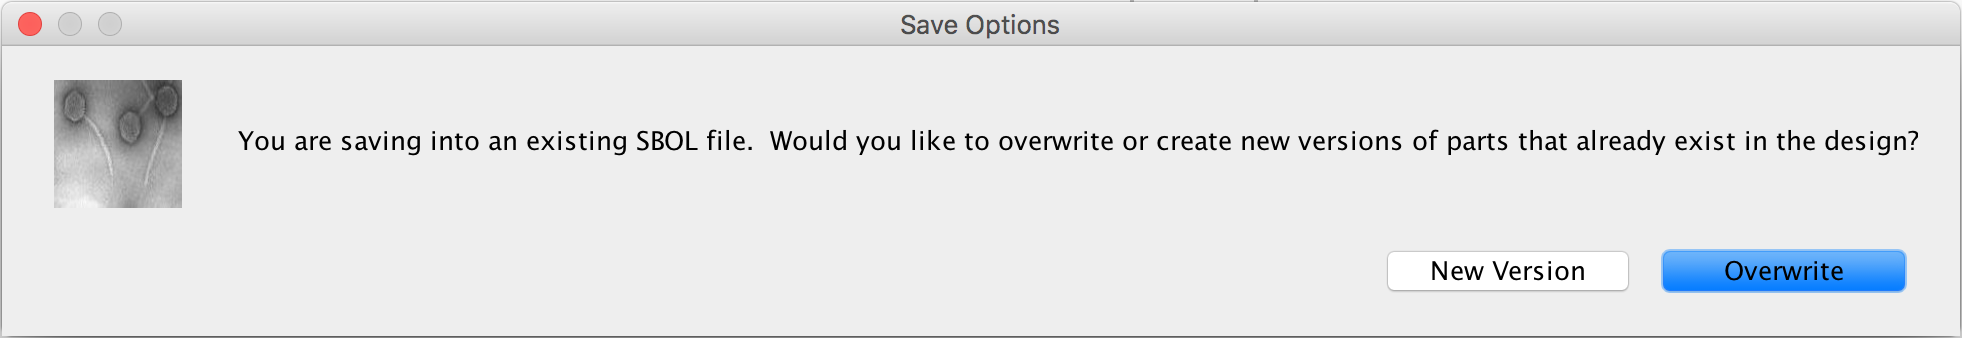
\includegraphics[width=160mm]{screenshots/PartSave}
\end{center}

\end{itemize}



\section{Model Editor}

\noindent
\begin{itemize}
\item Now that we have finished creating the genetic circuits that are part of this genetic toggle switch model, we can begin building the model. This tutorial will show how to model the genetic toggle switch using a hierarchical model, building two modules before the final model, so without further ado, let's begin with the LacI Inverter.

\subsection{LacI Inverter}
\item In order to begin creating our model, select the File menu, hover over New, and select Model. You could also use the keyboard shortcut control $\rightarrow$ M on the Windows and Linux versions or command $\rightarrow$ M on the Mac OS version.

\begin{center}
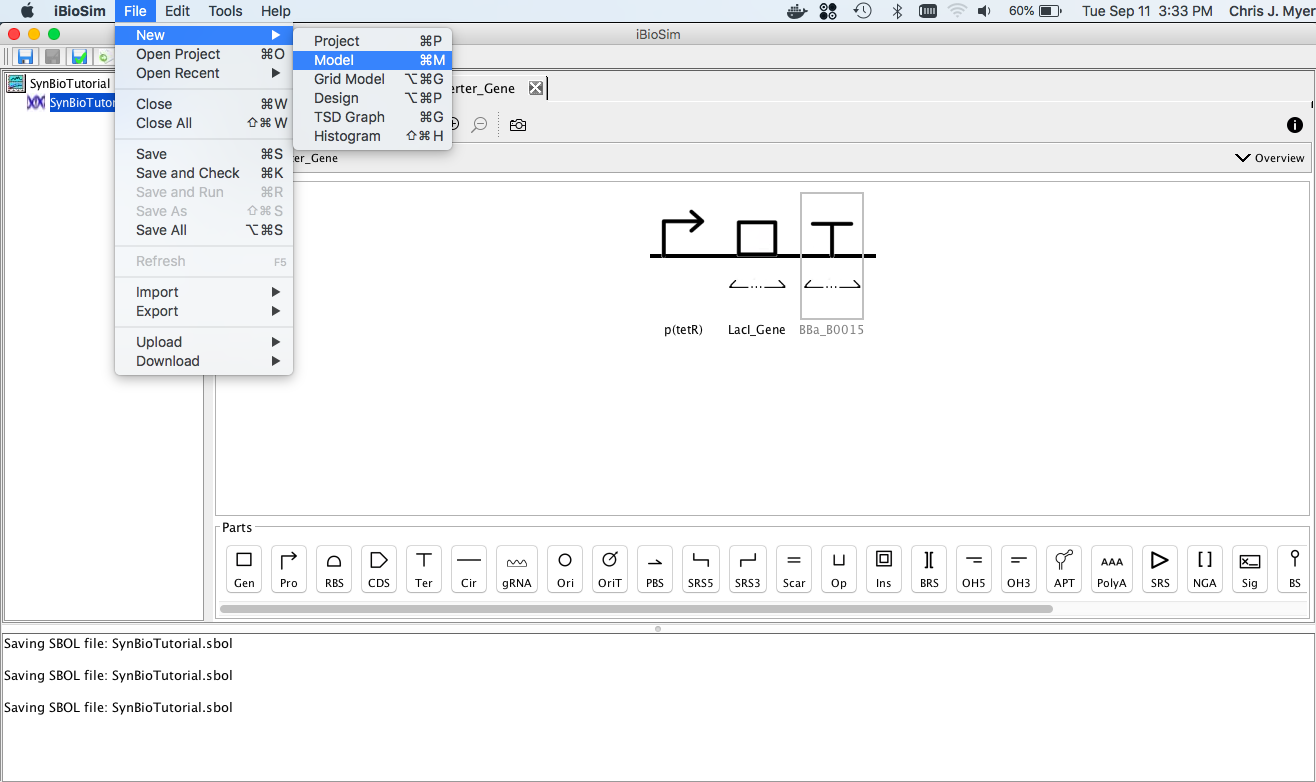
\includegraphics[width=160mm]{screenshots/newModel}
\end{center}

\item You will then be prompted to enter a Model ID. Enter LacI\_Inverter into the Model ID because this particular model will model the repression of the GFP (Green Fluorescent Protein) gene by the LacI protein.

\begin{center}
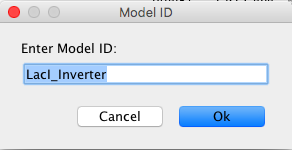
\includegraphics[width=75mm]{screenshots/ModelIdGT}
\end{center}

\item The next step is to add the proteins involved in this operon. In this particular model, there are three proteins; LacI, TetR, and GFP. So click on the Add Species icon \includegraphics{../gui/src/main/resources/edu/utah/ece/async/ibiosim/gui/icons/modelview/add_species_selected} on the tool ribbon and click on three different locations on the schematic canvas to create the three proteins.

\begin{center}
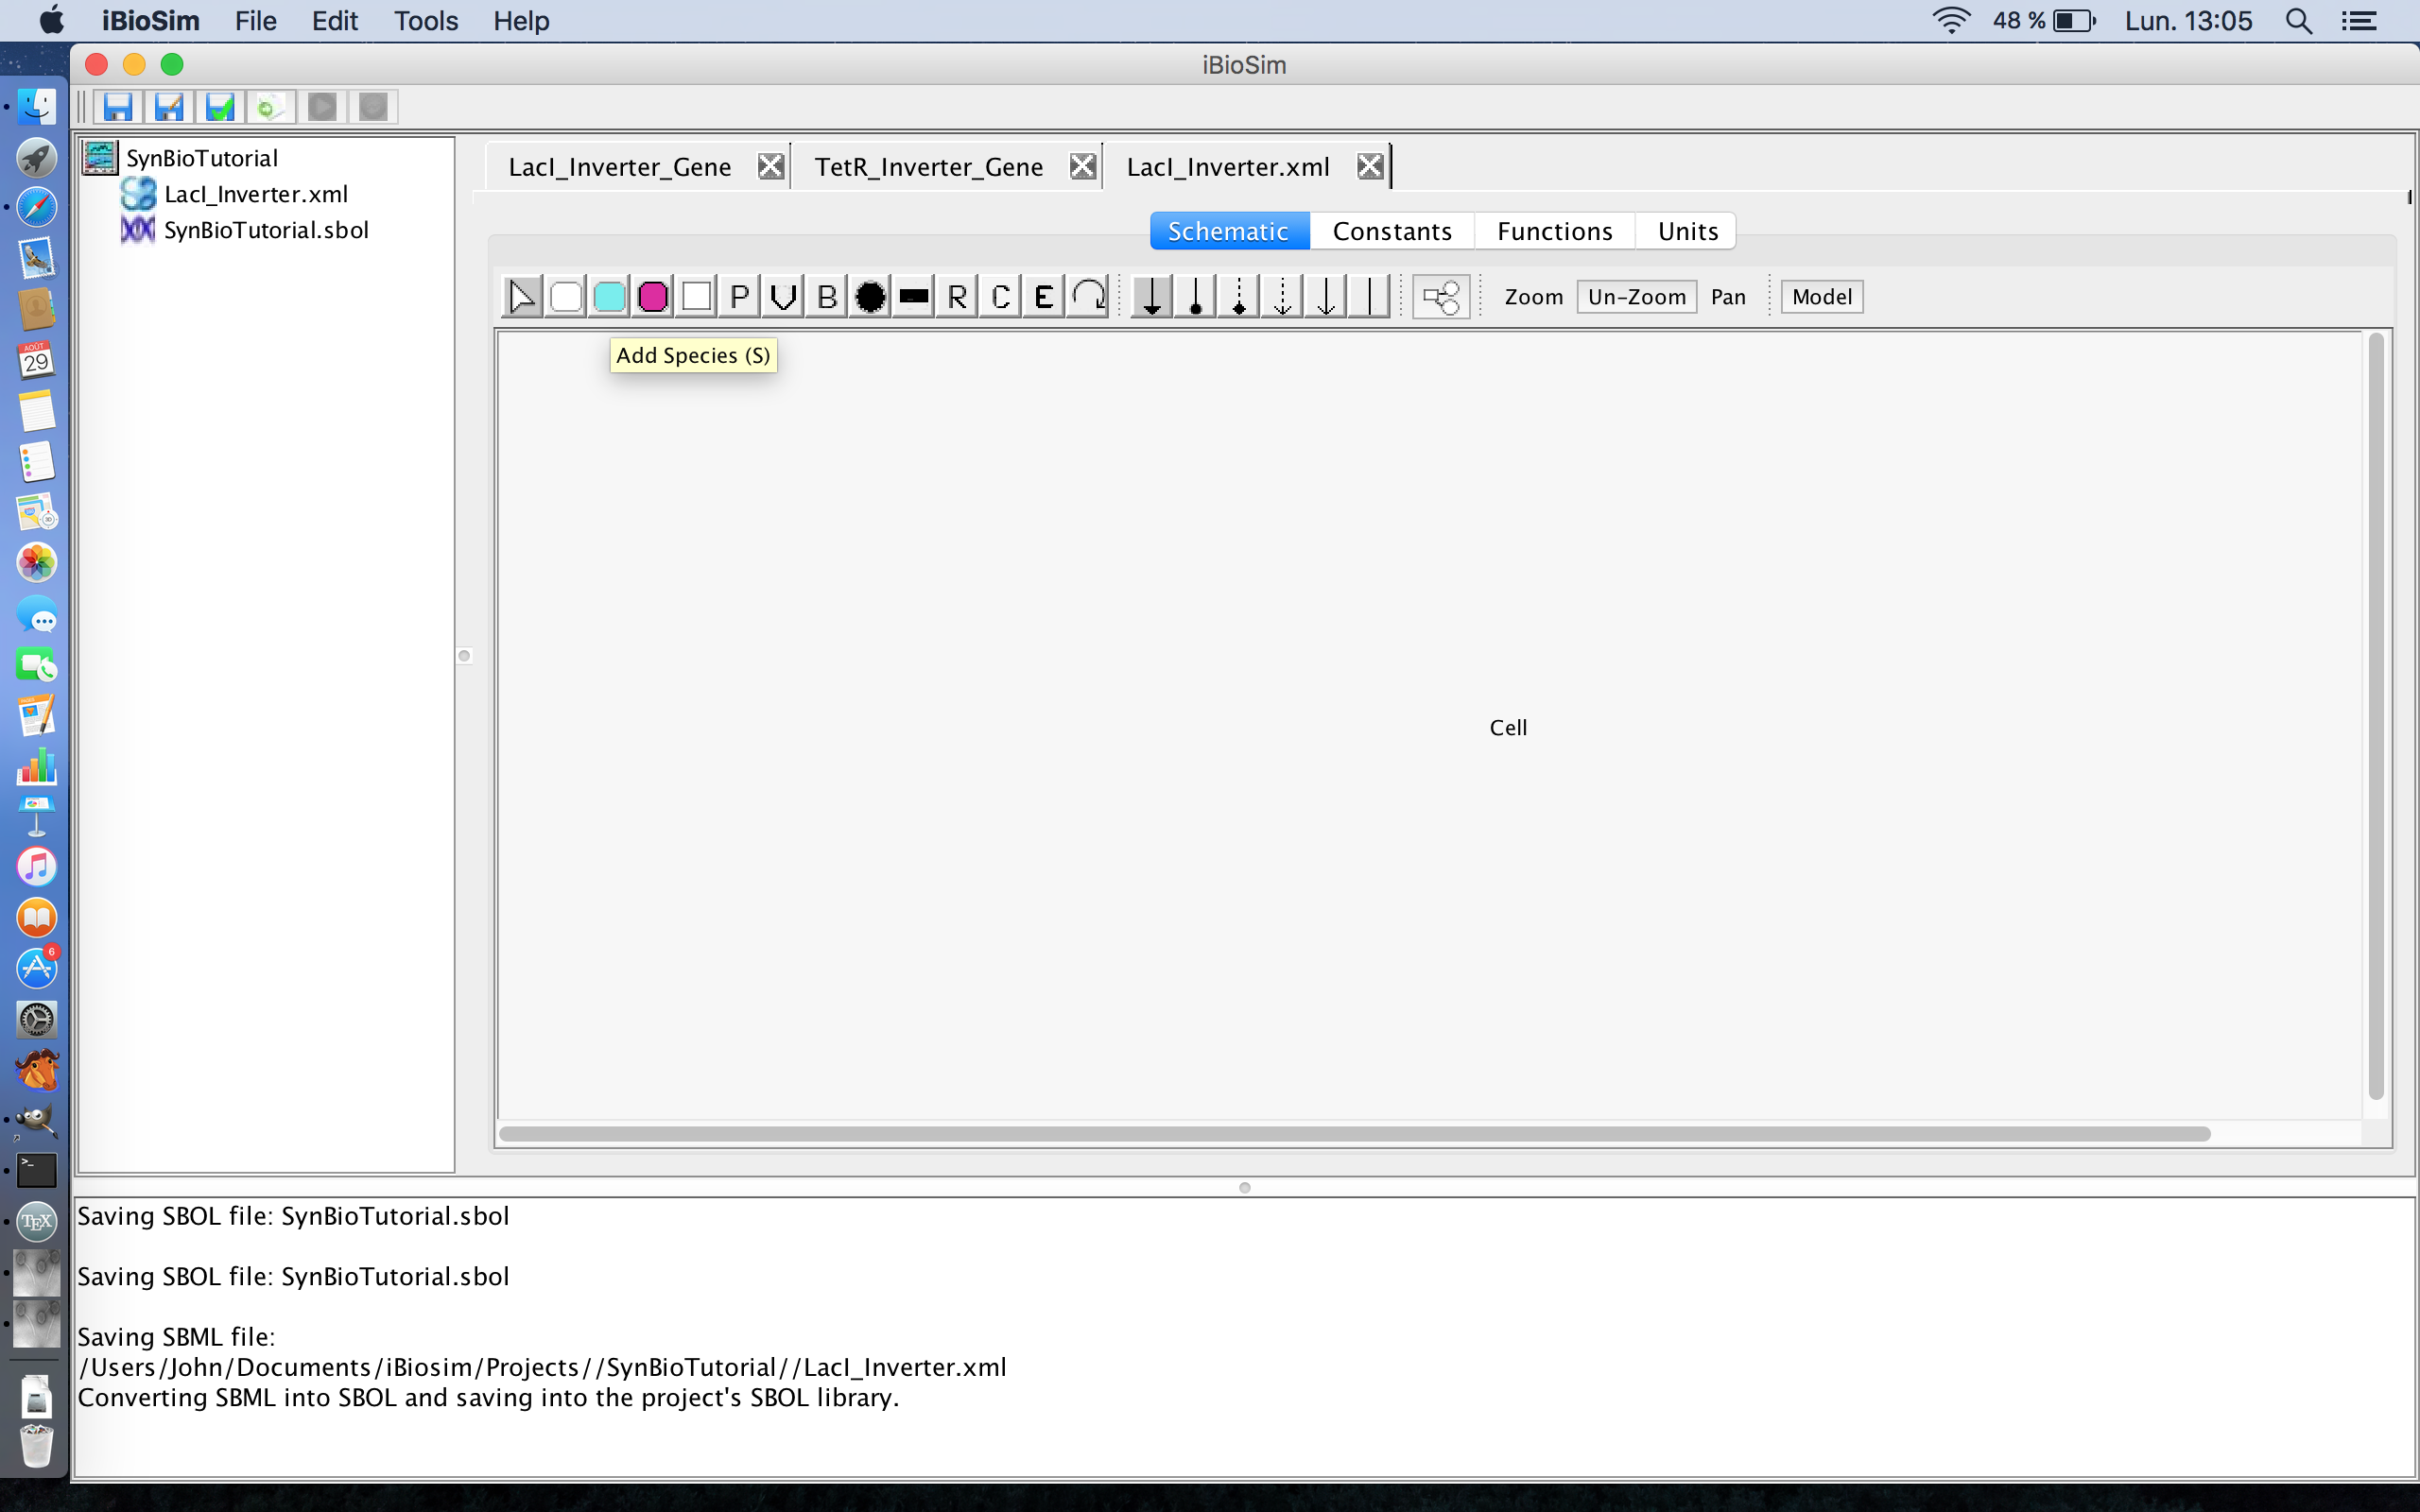
\includegraphics[width=160mm]{screenshots/schematicGT}
\end{center}

\begin{center}
\includegraphics[width=160mm]{"screenshots/Proteins Inserted"}
\end{center}

\item Next, select the cursor icon \includegraphics{../gui/src/main/resources/edu/utah/ece/async/ibiosim/gui/icons/modelview/select_mode_selected} from the tool ribbon and double-click on one of the proteins to open the Species Editor.

\begin{center}
\includegraphics[width=160mm]{"screenshots/Cursor Icon Selected"}
\end{center}

\begin{center}
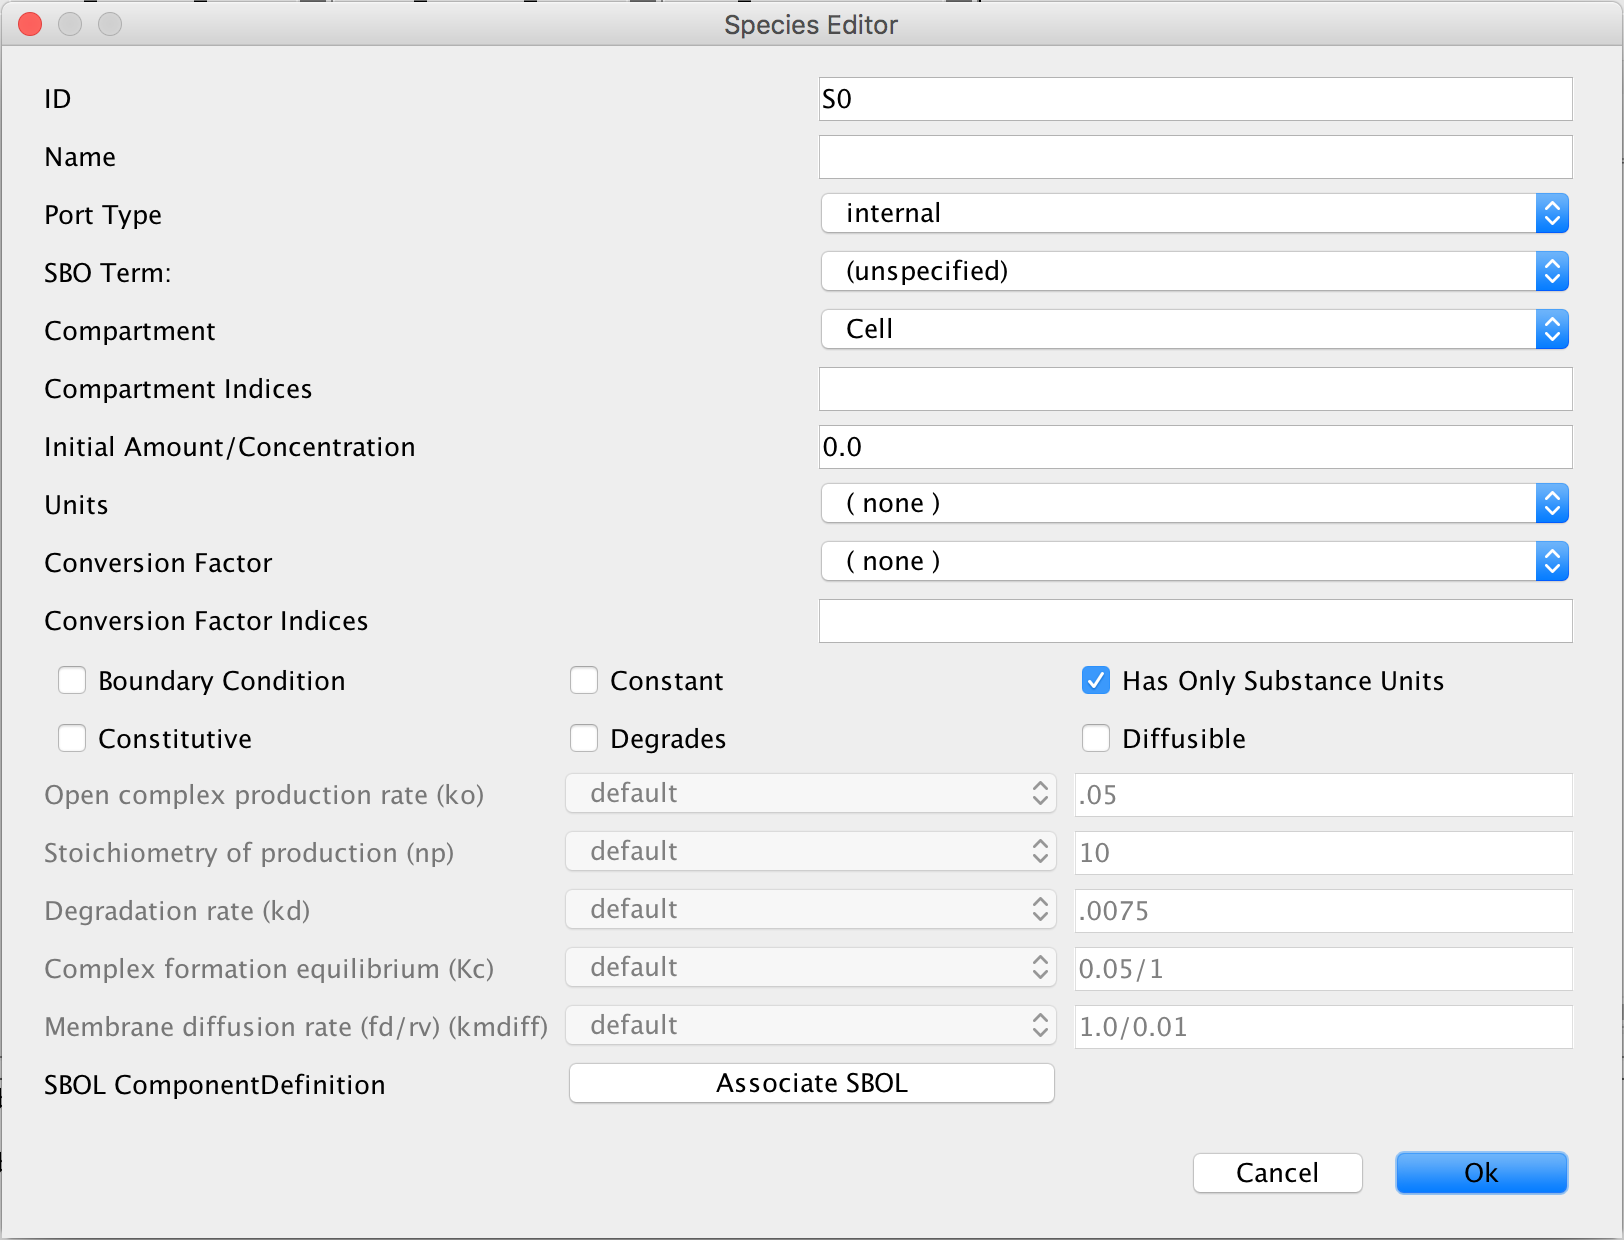
\includegraphics[width=110mm]{screenshots/speciesGT}
\end{center}

\item In the ID criterion, enter LacI.
\item Now, change, the port type to input. This specifies that the LacI protein will be imported into this model from a different model that will be created later.
\item Click Ok to save the entered criteria in the Species Editor.

\begin{center}
\includegraphics[width=110mm]{"screenshots/LacI Inverter LacI"}
\end{center}

\item Now, double-click on another of the proteins to open its Species Editor.
\item Enter TetR into the ID criterion of this protein.
\item This time, change the port type to output specifying that this protein will be exported into to another model that will be created later in this tutorial.
\item Finally, click Ok to save the entered criteria for this protein.

\begin{center}
\includegraphics[width=110mm]{"screenshots/LacI Inverter TetR"}
\end{center}

\item Now, double-click on the last protein to open its Species Editor.
\item Enter GFP into its ID criterion, and once again select output on the port type.
\item Now, click Ok to save the entered criteria.

\begin{center}
\includegraphics[width=110mm]{"screenshots/LacI Inverter GFP"}
\end{center}

\begin{center}
\includegraphics[width=160mm]{"screenshots/LacI Inverter Species Inserted"}
\end{center}

\item The next step is to add a promoter to this model to order to specify which genes are present in this operon, so click the promoter icon. \includegraphics{../gui/src/main/resources/edu/utah/ece/async/ibiosim/gui/icons/modelview/promoter_mode_selected} on the tool ribbon and click on the schematic canvas to add a promoter to the model.

\begin{center}
\includegraphics[width=160mm]{"screenshots/Promoter Icon Selected"}
\end{center}

\begin{center}
\includegraphics[width=160mm]{"screenshots/LacI Inverter Promoter Inserted"}
\end{center}

\item Now, select the cursor icon \includegraphics{../gui/src/main/resources/edu/utah/ece/async/ibiosim/gui/icons/modelview/select_mode_selected} again from the tool ribbon and double click the promoter to open the Promoter Editor.

\begin{center}
\includegraphics[width=110mm]{screenshots/promoterGT}
\end{center}

\item Enter pLac into the ID criterion because it is the promoter in the Lac operon.

\begin{center}
\includegraphics[width=110mm]{"screenshots/LacI Inverter pLac"}
\end{center}

\item Now click on Associate SBOL near the bottom of the Promoter Editor to open the SBOL editor in order to associate the LacI\_Inverter\_Gene made in Part Editor with this promoter. This will open the SBOL Association window.

\begin{center}
\includegraphics[width=75mm]{"screenshots/LacI Inverter Blank Associate SBOL"}
\end{center}

\item Click add to open the SBOL Browser in order to find the genetic circuit file created earlier in this tutorial. Scroll down the Component Definitions until you find the LacI\_Inverter\_Gene, then press Ok to add it to the SBOL Association window.

\begin{center}
\includegraphics[width=110mm]{"screenshots/SBOL Browser"}
\end{center}

\begin{center}
\includegraphics[width=110mm]{"screenshots/SBOL Browser pLac"}
\end{center}

\item Press Ok on the SBOL Association and on the Promoter Editor window to associate our LacI Inverter Gene genetic circuit with the pLac promoter.

\begin{center}
\includegraphics[width=75mm]{"screenshots/SBOL Association pLac"}
\end{center}

\item As you may now notice, the promoter tile has been replaced with a new grey tile that resembles a genetic circuit. This indicates that this promoter is now associated with an SBOL file. The next step is to show the interactions between the proteins and the promoter. The pLac promoter is repressible by LacI, so in order to show this relationship, first select the repression icon \includegraphics{../gui/src/main/resources/edu/utah/ece/async/ibiosim/gui/icons/modelview/inhibition_selected}.

\begin{center}
\includegraphics[width=160mm]{screenshots/RepressionArc}
\end{center}

\item In order to show that LacI represses the transcription of the TetR and GFP genes, hover over the LacI protein highlighting it. Now, while holding down the mouse button, draw a line connecting the LacI protein to the pLac promoter.

\begin{center}
\includegraphics[width=160mm]{"screenshots/Repression Arc Beginning"}
\end{center}

\begin{center}
\includegraphics[width=160mm]{"screenshots/Repression Arc Target"}
\end{center}

\begin{center}
\includegraphics[width=160mm]{"screenshots/Repression Arc Complete"}
\end{center}

\item To show that the promoter leads to the transcription and translation of the TetR and GFP genes, hover over the promoter and while holding down the mouse button and draw a line to the TetR protein and then do the same for the GFP genes.

\begin{center}
\includegraphics[width=160mm]{"screenshots/LacI Inverter Complete"}
\end{center}

\subsection{TetR Inverter}
\item The next step is to create the model of TetR repressing the LacI gene, so select the file menu and hover over New and then select Model. Enter TetR\_Inverter in the Model ID.

\begin{center}
\includegraphics[width=75mm]{screenshots/ModelTetRId}
\end{center}

\item Once again, it is necessary to add the proteins involved in this models, namely TetR and LacI, so select the Add Species icon \includegraphics{../gui/src/main/resources/edu/utah/ece/async/ibiosim/gui/icons/modelview/add_species_selected} from the tool ribbon and click on two different locations on the schematic canvas to create the two proteins.

\begin{center}
\includegraphics[width=160mm]{screenshots/TetRInverterSpecies}
\end{center}

\item Now, select the cursor icon \includegraphics{../gui/src/main/resources/edu/utah/ece/async/ibiosim/gui/icons/modelview/select_mode_selected} and double-click on one of the proteins to open the Species Editor. Enter TetR into the ID criterion and select input in the Port Type criterion to specify that TetR comes from the model that shall be created next and then click Ok.

\begin{center}
\includegraphics[width=110mm]{screenshots/TetRInverterTetR}
\end{center}

\item Now, double-click on the remaining protein to open its Species Editor, and enter LacI into the ID criterion and export into the Port Type criterion. In the Initial Amount/Concentration, type in 60 because this model starts out with the GFP gene suppressed.

\begin{center}
\includegraphics[width=110mm]{screenshots/TetRInverterLacI}
\end{center}

\item Next, as before, insert a promoter into the model, so that we can begin to establish the relationship between LacI and TetR. 

\begin{center}
\includegraphics[width=160mm]{screenshots/TetRInverterPromoter}
\end{center}

\item Then select the cursor icon \includegraphics{../gui/src/main/resources/edu/utah/ece/async/ibiosim/gui/icons/modelview/select_mode_selected} and double-click the promoter to open the promoter editor. In the ID criterion, type pTet because this is the TetR repressible promoter that leads to the translation and transcription of LacI.

\begin{center}
\includegraphics[width=110mm]{screenshots/TetRInverterpTet}
\end{center}

\item Now click the Associate SBOL button to open the SBOL Association window. This time however, select the Reverse Complement box because this gene is on the opposite side of the DNA as the previous two genes in the LacI Inverter model.

\begin{center}
\includegraphics[width=75mm]{screenshots/TetRInverterSBOL}
\end{center}

\item Once again, click the Add button to open the SBOL Browser. In the Component Definitions, scroll down to the TetR\_Inverter\_Gene made earlier in this tutorial.

\begin{center}
\includegraphics[width=110mm]{screenshots/TetRInverterSBOLBrowser}
\end{center}

\item Press Ok on the SBOL Browser menu, the SBOL Association window, and the Promoter Editor Window to associate the genetic circuit with the promoter.

\begin{center}
\includegraphics[width=160mm]{screenshots/TetRInverterStuffInserted}
\end{center}

\item Now, to show that TetR represses the transcription and translation of the LacI gene, select the repression icon \includegraphics{../gui/src/main/resources/edu/utah/ece/async/ibiosim/gui/icons/modelview/inhibition_selected} from the tool ribbon and draw a line from the TetR protein to the promoter. Then, to show pTet leads to the production of LacI, draw line from the pTet promoter to LacI.

\begin{center}
\includegraphics[width=160mm]{screenshots/TetRInverterComplete}
\end{center}

\subsection{Genetic Toggle Switch Model}
\item Now that these two models are completed, we can finally create the Genetic Toggle Switch model, so first, create a new model called GeneticToggle.

\begin{center}
\includegraphics[width=75mm]{screenshots/GeneticToggleID}
\end{center}

\item Make sure the cursor icon \includegraphics{../gui/src/main/resources/edu/utah/ece/async/ibiosim/gui/icons/modelview/select_mode_selected} is selected and double-click on the schematic canvas to open the Compartment Editor.
\item Deselect Is Mapped to a Port because this model encompasses the other two models that were just created (hierarchical model).
\item Now click Ok.

\item Then, the proteins involved in the Genetic Toggle, GFP, TetR, and LacI must be added to this model, so select the Add Species icon \includegraphics{../gui/src/main/resources/edu/utah/ece/async/ibiosim/gui/icons/modelview/add_species_selected} and click on the schematic canvas three times.

\begin{center}
\includegraphics[width=160mm]{screenshots/GeneticToggleThree}
\end{center}

\item Select the cursor icon \includegraphics{../gui/src/main/resources/edu/utah/ece/async/ibiosim/gui/icons/modelview/select_mode_selected} from the tool ribbon and double-click on one of the proteins to open the Species Editor, and then, enter LacI in the ID criterion. This time, leave the Port Type on internal because the LacI is not entering this model from somewhere else or going into another model. In addition, under Conversion Factor Indices, select Degrades to indicate that this protein degrades overtime. Then press Ok.

\begin{center}
\includegraphics[width=110mm]{screenshots/GTLacI}
\end{center}

\item Now, open the Species Editor for the other two proteins and enter TetR and GFP into their ID criterions. Under Conversion Factor Indices for both proteins, select degrades. Just like LacI, both of these proteins degrade over time in biological systems. Click Ok to save these criteria.

%\begin{center}
%\includegraphics[
\item It is now necessary to add the previous two models to this model, so select the Add Module icon \includegraphics{../gui/src/main/resources/edu/utah/ece/async/ibiosim/gui/icons/modelview/add_component_selected} from the tool ribbon and click on the schematic canvas.
\item Now select the LacI\_Inverter model and click Ok to add it to this model.
\item Click on the schematic canvas again and select the TetR\_Inverter to add it to this model.
\item Now, it is necessary to show the relationship between the models and proteins. First select the arrow icon and draw a line from the LacI protein to the LacI\_Inverter module to indicate that the LacI protein in this model is the inputted protein in the LacI\_Inverter model.
\item Now, draw a line from the LacI\_Inverter Module to the TetR protein.
\item Since there are two output ports, you must select the TetR protein port to continue in order to confirm that output TetR protein corresponds to the internal TetR protein in this model.
\item Now draw a line from the TetR protein to the TetR\_Inverter module to link the internal TetR protein in this model to the inputted TetR protein in the TetR\_Inverter model.
\item Next, connect the TetR\_Inverter module to the LacI protein to link the outputted LacI protein in the TetR\_Inverter model to this model.
\item Finally, draw a line from the LacI\_Inverter module to the GFP protein to link the outputted GFP protein in the LacI\_Inverter model to this model's internal GFP protein.
\item The next step is to add the inducers that flip this genetic toggle switch on and off, IPTG and aTc respectively, so select the Add Species icon  \includegraphics{../gui/src/main/resources/edu/utah/ece/async/ibiosim/gui/icons/modelview/add_species_selected} from the tool ribbon and click on two areas of the schematic canvas.
\item Now select the cursor icon \includegraphics{../gui/src/main/resources/edu/utah/ece/async/ibiosim/gui/icons/modelview/select_mode_selected} from the tool ribbon and double-click one of the proteins to open the Species Editor.
\item Enter IPTG in the ID criterion.
\item Under the Conversion Factor Indices, select Boundary Condition in order to specify that its concentration remains constant for the purposes of this model.
\item Click Ok to save the criteria.
\item Now double-click the remaining protein to open its Species Editor.
\item Enter aTc in the ID criterion and once again select Boundary Condition under the Conversion Factor Indices.
\item Click Ok to save the entered criteria.
\item In operons, an inducer works by binding to the repressor protein changing the shape of the protein, so it no longer binds to the DNA before the promoter. This can be represented in this model by forming complexes of IPTG and LacI as well aTc and TetR, so select the Add Species icon \includegraphics{../gui/src/main/resources/edu/utah/ece/async/ibiosim/gui/icons/modelview/add_species_selected} from the tool ribbon and click on two areas of the schematic canvas to create the complexes.
\item Now select the cursor icon \includegraphics{../gui/src/main/resources/edu/utah/ece/async/ibiosim/gui/icons/modelview/select_mode_selected} from the tool ribbon and double-click on one of the complexes to open the Species Editor.
\item Under the item criterion, type IPTG\_LacI to indicate that this is the complex formed by IPTG binding to LacI.
\item Under the Conversion Factor Indices, select Degrades because this complex over time in biological systems eventually degrades.
\item Now double-click the remaining complex to open its Species Editor, and label this one's ID as aTc\_TetR to indicate that this complex is formed by aTc binding to TetR.
\item Once again, under the Conversion Factor Indices, select Degrades for the same reason as IPTG\_LacI complex.
\item Now, it is necessary to show the relationship among the complex, the inducer, and repressor protein, so select the Complex Formation Icon \includegraphics{../gui/src/main/resources/edu/utah/ece/async/ibiosim/gui/icons/modelview/bio_activation_selected} and draw a line from IPTG to the IPTG\_LacI complex as well as a line from LacI to the IPTG to show that a complex is formed when IPTG binds to LacI.
\item Now, connect aTc to the aTc\_TetR complex as well as TetR to the aTc\_TetR complex to show that aTc and TetR form a complex when aTc binds to TetR.
\item The default Stoichiometry of binding for complex formation is 2. However, since these reactions only require one of each reactant to form one complex, the Stoichiometry of binding for these reactions is 1. So, select the cursor icon \includegraphics{../gui/src/main/resources/edu/utah/ece/async/ibiosim/gui/icons/modelview/select_mode_selected} and double-click one of the lines that connects a reactant to one of the complexes and under Stoichiometry of binding (nc), change default to custom and change the parameter from 2 to 1.
\item Repeat the above step for each of the lines connecting the reactants to the two complexes.
\item The final step is to add events to change the amount of IPTG and aTc present in the system to turn the genetic toggle switch on and off, so select the Event Icon \includegraphics{../gui/src/main/resources/edu/utah/ece/async/ibiosim/gui/icons/modelview/event_mode_selected} and click on the schematic canvas to add an event and open the Event Editor.
\item Under the ID criterion, label the event IPTG\_High because this event will increase the amount of IPTG in the system at a specific time.
\item Under the Delay criterion, type 2000 to specify the amount of time before the event will be allowed to trigger, so that the switch starts in the off position for a period of time.
\item Now go up to the Trigger condition and type true to specify that the event will trigger immediately at time equals 2000.
\item Next, click on Add Assignment to open the Event Assignment Editor to specify what the event shall do when it triggers.
\item In the Event Assignment Editor, set the variable to IPTG because this event will increase the amount of IPTG present in the system.
\item Next, set the Assignment to 60 in order to increase the IPTG present from 0 to 60 because enough IPTG must be present in the system to stop the repression of the TetR and GFP genes by LacI to turn the switch on.
\item Now, click on the Add button in the Event Assignment Editor to add this assignment to the editor.
\item Click on the Add button in the Event Editor to create the event.
\item The next event that needs to be created is necessary to lower the IPTG value back to zero in order to show that the switch remains on even when the inducer is no longer present, so click on another space on the schematic canvas to create another event.
\item Under the ID criterion, type IPTG\_Low because this event will lower the IPTG present in the system back to 0.
\item Under the Delay criterion, set the value to 4000 because this event should occur after some time after the previous event raises the IPTG value.
\item Set the Trigger condition to true, so the event will trigger at time 4000.
\item Now, the purpose of the event must be set, so click the Add Assignment to open the Event Assignment Editor.
\item Set the variable to IPTG again because this event will lower the concentration of IPTG, and set the Assignment criterion to 0 to lower the IPTG in the system back from 60 to 0.
\item Click on the Add button to finalize the assignment, and then click on the Add button in the Event Editor to create the event.
\item The next step is to create the events that turn the switch off, so click in another location in the schematic canvas to open the Event Editor to create another event.
\item Under the ID criterion, type aTc\_High because this event will increase the amount of aTc present in the system to turn the switch off.
\item Set the Delay criterion for this event to 6000 because it should occur after the previous events, and once again, set the Trigger criterion to true so the event occurs at 6000.
\item Click on Add Assignment so that the event increases the aTc concentration at time equals 6000.
\item Set the variable to aTc this time because that is the molecule concentration being changed.
\item Under the Assignment criterion, set the value to 60 to raise the aTc concentration from 0 to 60.
\item Click Add to add this assignment to the event, and then click Add in the Event Editor to create the event.
\item The last event that needs to be created will essentially reset the system back to its starting state, so once again, click another place on the schematic canvas to create another event.
\item Under the ID criterion in the Event Editor, type aTc\_Low because this event will lower aTc back to 0 resetting the system back to the way it was at time equals 0.
\item Under the Delay criteria, set the value to 8000, so the event occurs after the previous three events.
\item Now, set the Trigger criterion to true, so the event triggers right at time equals 8000.
\item Click Add Assignment to open the Event Assignment Editor in order to specify what the event does.
\item Set the variable to aTc because this event will lower the concentration of aTc, and set the Assignment criterion to 0 to lower the aTc concentration back to 0.
\item Click Add to add the assignment to the Event, and then click Add in the Event Editor to create the event.
\item Now select the File Menu and click Save.
\end{itemize}

Let us know see how to create a new model using the Model Editor.  First, select New $\rightarrow$ Model from the File menu as shown below. You will then be prompted to enter a model ID.  Enter {\tt LacI\_Inverter}.  At this point, a Model editor will open in a new tab.

\begin{center}
\includegraphics[width=80mm]{screenshots/newModel}
\end{center}

\begin{center}
\includegraphics[height=75mm]{screenshots/ModelIdGT}
\end{center}

\begin{center}
\includegraphics[width=160mm]{screenshots/schematicGT}
\end{center}

To add a chemical species, select the Add Species icon \includegraphics{../gui/src/main/resources/edu/utah/ece/async/ibiosim/gui/icons/modelview/add_species_selected} and click on the schematic canvas  (note that this can also be done using the Edit menu or the hotkeys shown in this menu).  This will drop a new species with default ID and other values.  You may change these defaults by clicking on the selection icon 
\includegraphics{../gui/src/main/resources/edu/utah/ece/async/ibiosim/gui/icons/modelview/select_mode_selected}, and
double-clicking on the species to open the Species Editor.  In this case, let us change the ID to LacI and change the Port type to \emph{input}.  We will leave all the other values at their default values.  The port type of input indicates that this species will be used as an input for the LacI inverter.   
Note that while in the select mode, you can also select an object in the schematic and move it by moving the mouse while holding the left mouse button.  Pressing the right mouse button while an object is selected brings up a menu that allows you to delete an object from the schematic.  Repeat the steps above to add TetR and GFP species.  Give these species port type of \emph{output}. 

\begin{center}
\includegraphics[width=160mm]{screenshots/speciesGT}
\end{center}

% Add another species for the CI dimer molecule.  The next step is to add a complex-formation reaction to convert CI monomers into CI dimers.  Select the complex formation icon \includegraphics{../gui/src/main/resources/edu/utah/ece/async/ibiosim/gui/icons/modelview/bio_activation_selected}, highlight the CI species, and, while holding the mouse button, stretch the complex formation arc to the S1 species.  Next, edit this species to set its ID to CI2 and select that it degrades.  This species is created using a complex-formation reaction with an equilibrium constant of 0.1.  Change default to custom for the complex formation equilibrium and set it to this value as shown below.

% \begin{center}
% \includegraphics[width=160mm]{screenshots/species2} 
% \end{center}

% If you double-click on the complex formation arc, an influence editor will open which indicates that this is a complex formation arc and the stoichiometry of binding (i.e., the number of molecules of the source species used to construct the sink species) is 2.  The default in this case is correct as it does take two molecules of CI to make CI2.

% \begin{center}
% \includegraphics[width=160mm]{screenshots/complex} 
% \end{center}

Next, let's add the pLac promoter, which initiates transcription of the gene that produces the proteins TetR and GFP.  To do this, select the promoter icon \includegraphics{../gui/src/main/resources/edu/utah/ece/async/ibiosim/gui/icons/modelview/promoter_mode_selected} and click on the schematic canvas to drop the promoter with a default ID and parameter values.  Double-click on the promoter to bring up the promoter editor.  Change the ID to pLac.
 
\begin{center}
\includegraphics[width=160mm]{screenshots/promoterGT} 
\end{center}

The pLac promoter is repressed by the LacI species.  To create this relationship, select the repression arc icon 
\includegraphics{../gui/src/main/resources/edu/utah/ece/async/ibiosim/gui/icons/modelview/inhibition_selected}, highlight the LacI species, and, while holding the mouse button, stretch the repression arc to the pLac promoter.  
%% Next, double-click on the repression arc to bring up the influence editor.  

\begin{center}
\includegraphics[width=160mm]{screenshots/repressionGT} 
\end{center}

As mentioned earlier, the pLac promoter initiates the production of the TetR and GFP species.  Highlight the pLac promoter and, while holding the mouse button, stretch the production arc to the TetR species.  Repeat these steps to create a production arc between the pLac promoter and GFP species.  Note that any regulation icon can be selected for this because all arcs from promoters to species are always production arcs.  

\begin{center}
\includegraphics[width=160mm]{screenshots/productionGT}
\end{center}

Let us now annotate the LacI inverter with its DNA sequence.  To do this, we will need to first import some annotated sequence data stored using the \emph{synthetic biology open language} (SBOL).  Select the File $\rightarrow$ Import $\rightarrow$ SBOL File menu option as shown below.  This will bring up a file browser.  You will need to find the location where {\tt iBioSim} is installed, and the file you want to import should be located in {\tt iBioSim/docs/SynBioTutorial/SBOL/GeneticToggle.sbol}.  

\begin{center}
\includegraphics[width=60mm]{screenshots/importSBOL}
\end{center}

Next, click on the Model button in the schematic editor which brings up the Model editor shown below.  

\begin{center}
\includegraphics[width=160mm]{screenshots/ModelEditorGT}
\end{center}

Next, click on the Associate SBOL button, highlight the placeholder for the DNA component, and click the Remove button.  Then, press the Add button which will open the SBOL browser shown below.  In the list of DNA components, scroll down to the component named pIKERightCassette\_1, select it, and press OK.

\begin{center}
\includegraphics[width=160mm]{screenshots/SBOLBrowserGT}
\end{center}

The SBOL association editor should now show this DNA component as being associated with this model.  We could now add more components, if we wish, but only one is needed for this, so press Ok.  We are now done with the LacI inverter model, so let's make sure the model is saved by either clicking on the Save icon \includegraphics{../gui/src/main/resources/edu/utah/ece/async/ibiosim/gui/icons/save} or selecting the Save option from the File menu.

\begin{center}
\includegraphics[width=160mm]{screenshots/SBOLAssociationGT}
\end{center}

Next, repeat the steps above to create a TetR\_Inverter model.  The TetR inverter has input TetR and output LacI.  In the TetR inverter, TetR represses the production of LacI.  To indicate this, select the repression icon \includegraphics{../gui/src/main/resources/edu/utah/ece/async/ibiosim/gui/icons/modelview/inhibition_selected}, highlight the TetR species and stretch the arc to the LacI species.  This action creates an implicit promoter P0 that is repressed by TetR and initiates production of LacI.  When you associate SBOL with this model, select the pIKELeftCassette\_1 component, and select for it to be put on the Minus Strand by checking the box on the SBOL association window.  Do not forget to save this model either by clicking on the Save icon \includegraphics{../gui/src/main/resources/edu/utah/ece/async/ibiosim/gui/icons/save} or selecting the Save option from the File menu.

\begin{center}
\includegraphics[width=160mm]{screenshots/implicitPromoterGT}
\end{center}

Now, let us put these genetic inverters into a new model called GeneticToggle.
This model will be the top-level model, and all elements of this model will be enclosed in this model's \emph{compartment}.  Compartments are the membrane-enclosed regions where species can be found and reactions take place.  {\tt iBioSim} creates a default compartment initially with the ID of Cell.  If you click on the schematic within the Cell compartment, it brings up the compartment editor.  Uncheck the ``Is Mapped to a Port''.  This indicates that this compartment should be enclosing this model and not replaced when instantiated in a larger model.  Once you press OK, you will notice that the compartment now has rounded corners to indicate that this is membrane enclosed by the compartment Cell.

\begin{center}
\includegraphics[width=160mm]{screenshots/compartmentGT}
\end{center}

Now, lets add the LacI\_Inverter component to this model.  Select the Add Component icon \includegraphics{../gui/src/main/resources/edu/utah/ece/async/ibiosim/gui/icons/modelview/add_component_selected} and click on the Schematic canvas opening the Add Component(s) window.  In this window, browse the combo box, if necessary, to find your LacI\_Inverter model.  Pressing OK will then add it to your schematic.  Repeat these steps to add the TetR\_Inverter.

\begin{center}
\includegraphics[width=160mm]{screenshots/subModelGT}
\end{center}

The next step is to connect the components through their species.   To do this, add species to the model for LacI, TetR, and GFP.  Mark that each of these species degrades, and set the initial amount of LacI to 60.  The degrades checkbox means that when this model is analyzed a default degradation reaction will be created which has a rate of 0.0075.  Next, highlight the LacI species and stretch a connection to the LacI\_Inverter connecting it to its LacI input port.  Next, highlight the LacI\_Inverter and stretch to the TetR species.  In this case, since there are two output ports, you must select the TetR output port is the one desired.  Next, highlight the TetR species and stretch to the TetR\_Inverter to connect to the TetR input port.  Next, highlight the TetR\_Inverter and stretch to the LacI species to connect it to its LacI output port.  Finally, highlight the Lac\_Inverter and stretch to the GFP species being sure to select to connect to its GFP output port.  

\begin{center}
\includegraphics[width=160mm]{screenshots/addConnectionGT}
\end{center}

By instantiating these models together, the SBOL associated with each component will now be composed as well.  To add some description for this composite DNA component, click on the Model button, followed by the Associate SBOL button on the Model Editor, and finally the Edit Composite button on the SBOL Association window.  You can now add an ID, Name, and Description for this composite DNA component as shown below.  

\begin{center}
\includegraphics[width=160mm]{screenshots/compSBOLDesc}
\end{center}

Next let us add the complex formation reactions that sequester LacI and TetR preventing them from acting as repressors.  First, add the small molecule species IPTG and aTc.  Select \emph{boundary condition} to indicate they are replenished inputs to the system.  Next, add the complex species IPTG\_LacI and aTc\_TetR and mark that they degrade.  Now, select the complex formation icon \includegraphics{../gui/src/main/resources/edu/utah/ece/async/ibiosim/gui/icons/modelview/bio_activation_selected}, highlight the IPTG species, and, while holding the mouse button, stretch the complex formation arc to the IPTG\_LacI species.  Repeat this step to connect complex formation arcs between LacI and this complex, as well as from aTc and TetR to the aTc\_TetR complex.  Finally, click on the selection icon 
\includegraphics{../gui/src/main/resources/edu/utah/ece/async/ibiosim/gui/icons/modelview/select_mode_selected}, and
double-click on each complex formation to open the Influence Editor.  In this editor, change the Stoichiometry of binding (nc) from 2 to 1 by first changing ``default'' to ``custom'' then editing the value.

\begin{center}
\includegraphics[width=160mm]{screenshots/complexGT}
\end{center}

The final step in the model creation is to add some discrete events to change the amounts of IPTG and aTc, so we may see the genetic toggle switch change state during simulation.  First, select the event icon \includegraphics{../gui/src/main/resources/edu/utah/ece/async/ibiosim/gui/icons/modelview/event_mode_selected}, and click on the schematic to add an event.  This action opens the event editor.  In this editor, create an event with ID ``IPTG\_High'', a trigger of ``true'', and a delay of 2000.  Next, click on Add Assignment to bring up the Event Assignment Editor.  In this editor, select the variable IPTG and provide the assignment of 60.  Press the Add button to add the assignment and the Add button to add the event.  This event will cause the amount of IPTG to change to 60 molecules after 2000 seconds of simulation time.  Repeat these steps to create an ``IPTG\_Low'' event with a delay of 4000 which assigns 0 to IPTG, an ``aTc\_High'' event with a delay of 6000 which assigns 60 to aTc, and finally an ``aTc\_Low'' event with a delay of 8000 which assigns 0 to aTc.

\begin{center}
\includegraphics[width=160mm]{screenshots/eventGT}
\end{center}

You should now have a complete model of the genetic toggle switch that looks like the one below (though locations of elements may be different).  Make sure the model is saved by either clicking on the Save icon \includegraphics{../gui/src/main/resources/edu/utah/ece/async/ibiosim/gui/icons/save} or selecting the Save option from the File menu.

\begin{center}
\includegraphics[width=160mm]{screenshots/saveGT}
\end{center}

\section{SBOL Browser}

As mentioned above, a composite DNA component has been constructed for the entire genetic toggle switch.  To see this component, click on the GeneticToggle.sbol file in the list of project files to open the SBOL browser.  On the right side, scroll down and select the DNA component that you named MyGeneticToggle.  You will now see the complete annotated DNA sequence for this component.  Note how the pIKELeftCassette\_1 has been put on the minus strand while the pIKERightCassette\_1 follows it on the positive strand.

\begin{center}
\includegraphics[width=160mm]{screenshots/SBOLBrowserGT2}
\end{center}

\section{Analysis Tool}

This section describes how to analyze the model just created.  The first step is to create an analysis view.  To do this, right-click on the model file and select Create Analysis View.  Enter the analysis ID {\tt GeneticToggle} or just press enter.  At this point, a new analysis view should open.  You should also notice that an icon appears next to your model file.  When you click on this, it will show you all of the analysis and learn views associated with this model.

\begin{center}
\includegraphics[height=60mm]{screenshots/createAnalysisViewGT}\\
\includegraphics[width=160mm]{screenshots/analysisViewGT}
\end{center}

In order to perform analysis, the analysis tool first converts the model into a detailed reaction-based model.  There are three different ways to see the reaction-based model that is produced.  If GraphViz is installed on your computer, you can select Network for your Simulation Type.  Then, either press the Save and Run icon \includegraphics{../gui/src/main/resources/edu/utah/ece/async/ibiosim/gui/icons/run-icon} or select the Save and Run option from the File menu.  The result will be a GraphViz window that will open to show the reaction-based model such as the one shown below for our example.  If it does not open in GraphViz, make sure that you have files with the {\tt .dot} file extension associated with GraphViz on your computer.  You can also view the model in a web browser by selecting Browser for your simulation type.  In this case, you should ensure that you have files with the {\tt .xhtml} extension associated with your favorite browser.  Finally, you can save the reaction-based model by selecting Model as your simulation type.  In this case, you must provide a new model ID.  This new model will appear in your project and it can be opened in the Model Editor.  Since this model does not include any layout information, you will need to either lay it out by hand or using one of the default layout routines selectable using the Apply Layout icon    \includegraphics{../gui/src/main/resources/edu/utah/ece/async/ibiosim/gui/icons/modelview/choose_layout_selected}.

\begin{center}
\includegraphics[width=160mm]{screenshots/viewNetworkGT}
\end{center}

\begin{center}
\includegraphics[width=160mm]{screenshots/viewBrowserGT}
\end{center}

\begin{center}
\includegraphics[width=160mm]{screenshots/reactionModelGT}
\end{center}

As you can see, this model is quite complex.  A simple model can be generated by selecting Abstraction to reduce the model using reaction-based abstractions based on the quasi-steady state assumption.  The abstracted model shown below is reduced from 15 species and 13 reactions to just 5 species and 5 reactions.  

\begin{center}
\includegraphics[width=160mm]{screenshots/reactionModelAbsGT}
\end{center}

Now, go back to the simulation options tab.  Here, make sure that Abstraction is still selected, change the simulation type back to ODE, the simulator to Runge-Kutta-Fehlberg,  the time limit to 10000.0, the print interval to 100.0, and enter a Simulation ID of {\tt ode}.  Then, either press the Save and Run icon \includegraphics{../gui/src/main/resources/edu/utah/ece/async/ibiosim/gui/icons/run-icon} or select the Save and Run option from the File menu.
After the simulation completes, click on the TSD Graph tab.  Double-click on the graph to bring up the graph editor.
Open the {\tt ode} simulation, highlight Average, select aTc, IPTG, and GFP, change the Title to ``ODE Simulation Results'', change the X-Axis Label to ``Time (seconds)'', and change the Y-Axis Label to ``Number of Molecules''.  
Press the OK button.  

\begin{center}
\includegraphics[width=160mm]{screenshots/odeSimGT}\\
\includegraphics[width=160mm]{screenshots/odeResultsGT}\\
\includegraphics[width=160mm]{screenshots/odeSimResultsGT}
\end{center}

Graphs can be exported in a variety of formats including:
\begin{itemize}
\item Time series data format (tsd).
\item Comma separated value (csv).
\item Column separated data (dat).
\item Encapsulated postscript (eps). 
\item Joint Photographic Experts Group (jpg). 
\item Portable document format (pdf).
\item Portable network graphics (png). 
\item Scalable vector graphics (svg).
\end{itemize}
In order to export a graph, you can either click on the Export icon \includegraphics{../gui/src/main/resources/edu/utah/ece/async/ibiosim/gui/icons/export} or select one of the graph export options from the File menu.  When using the Export icon, the type of file exported will depend on the extension provided to the file name.  Click on the Export icon, browse to a location on your file system, and enter the file name of {\tt ode.pdf} to create a PDF file for your graph.

\begin{center}
\includegraphics[height=60mm]{screenshots/exportTSD}
\end{center}

Now, select the Simulation Options tab again, select {\tt Monte Carlo}, change the simulator SSA-Direct, the number of runs to 100, set the simulation ID to {\tt ssa}, and click on the Save and Run icon.  Click on the TSD Graph tab.  Double-click on the graph to bring up the graph editor.  Click on Deselect All to remove the plotted points.  Open the {\tt ssa} simulation directory, and highlight {\tt run-1}.  Select aTc, IPTG, and GFP, and change the title to ``SSA Simulation Results''. Press the OK button.  Click on the Export icon and enter the file name {\tt ssa-1.pdf}.  Repeat these steps to generate graphs for the average ({\tt average.pdf}).

\begin{center}
\includegraphics[width=160mm]{screenshots/ssaSimGT}\\
\includegraphics[width=160mm]{screenshots/ssaResultsGT}\\
\includegraphics[width=160mm]{screenshots/ssaSimResultsGT}
\end{center}

Another way to view simulation results is on the schematic.  To do this, click on the schematic tab.  At the bottom of the window, select the Choose Simulation button, which brings up a window with all the simulations in this analysis view.  Open the {\tt ssa} directory, select {\tt run-1.tsd}, and press OK. 

\begin{center}
\includegraphics[width=160mm]{screenshots/chooseSimGT}
\end{center}

Now, click on the GFP species, which brings up the Edit Species window.  Select the Appearance tab.  Here you can select how you want the species to appear as you playback the simulation.  You can have it change color, size, and/or opacity on a gradient.  You can also select the range of molecule counts to specify the ends of the gradient(s).  Finally, you can indicate that these selections are either for this species or all species in the model.  For our example, let's make GFP  follow a green color gradient, IPTG follow a blue color gradient, LacI follow a cyan color gradient, aTc follow a red color gradient, and TetR follow a magenta gradient.
\begin{center}
\includegraphics[width=160mm]{screenshots/editSpeciesAppearanceGT}
\end{center}

Once you have made your selections, you can now play back the simulation.  You can either single-step the simulation by pressing the \includegraphics{../gui/src/main/resources/edu/utah/ece/async/ibiosim/gui/icons/modelview/movie/single_step} icon or play continuously by pressing the \includegraphics{../gui/src/main/resources/edu/utah/ece/async/ibiosim/gui/icons/modelview/movie/play} icon.  The playback can also be paused by pressing the \includegraphics{../gui/src/main/resources/edu/utah/ece/async/ibiosim/gui/icons/modelview/movie/pause} icon and restarted by pressing the  \includegraphics{../gui/src/main/resources/edu/utah/ece/async/ibiosim/gui/icons/modelview/movie/rewind} icon. 

\begin{center}
\includegraphics[width=160mm]{screenshots/movieViewGT}
\end{center}

\section{Grid Models}

In the last example, we will build a model with a grid. 
%First, edit the CII species and make it diffusible, and save the model.  
Create a grid model using the File $\rightarrow$ New $\rightarrow$ Grid Model menu, and name the new model {\tt Population}.  In the create grid window shown below, select your copy of your GeneticToggle model and change the number of rows and columns to 5.  

\begin{center}
\includegraphics[width=60mm]{screenshots/createGridGT}
\end{center}

The schematic in a grid model is a bit different.  It includes a grid in which each location can be empty or contain exactly one component.  Only components can be added to grids.

\begin{center}
\includegraphics[width=160mm]{screenshots/gridModelGT}
\end{center}

Next, right-click on the Population model and create an analysis view.  Select Abstraction, Monte Carlo, and the SSA-Direct simulator.  Set the time limit to 10000 with a print interval of 100, change the number of runs to 1, and perform the simulation.  Now, go to the schematic tab and press the Choose Simulation button to select run-1.tsd.  Click on one of the genetic toggle switch models to bring up the Edit Species editor.  Select the GFP species and a green color gradient, and apply to all components with this model.  Now, play back the simulation to see the toggle switches turn on and off.

\begin{center}
\includegraphics[width=160mm]{screenshots/gridSimGT}
\end{center}

% When you create a reaction-based model for a grid during analysis, reactions are created to move the diffusible species between the grid locations to provide a coarse form of spatial modeling.  If the component within a grid location is enclosed in a compartment membrane (indicated by the rounded corners), the model generated also includes reactions to diffuse the species in and out of the compartment.  In the analysis schematic, you can visualize your grid models by clicking on the component in the grid and selecting the species that you would like to see.  For each such species, you can set its color, size, and/or opacity gradient.  You can also copy these settings to all like models in your grid.  Finally, you can click on the area outside of the component within the grid to allow you to also visualize the species that are in the medium.

\begin{center}
\includegraphics[width=160mm]{screenshots/compAppearancesGT}
\end{center}

\begin{center}
\includegraphics[width=160mm]{screenshots/gridSimResultsGT}
\end{center}

\end{document}

Using the schematic tab, you can also adjust initial values and parameters allowing one to perform simulations to determine the effect of these changes.  Clicking on any species, promoter, reaction, or influence brings up the corresponding editor.  To change a value, switch the corresponding combo box to modified, which will then allow you to change the value.  For example, as shown below, we have reduced the degradation rate for CI to 0.00075.  Now, rerun the simulation and observe the change in the simulation data.

\begin{center}
\includegraphics[width=160mm]{screenshots/paramEdit}
\end{center}

In addition to making single changes, you can also sweep a value as shown below.   When you click on the Sweep button, it brings up a window where you can select the start value, the stop value, and the step value.  Using the values shown below for this example, simulations are generated using degradation rates of 0.001, 0.003, 0.005, and 0.007.  The level indicates how the sweep should perform when multiple variables are swept at the same time.  Variables at the same level are changed at the same time.  Furthermore, all variables on level 2 are stepped through all their values before changing the values of those variables on level 1.  After the values on level 1 are changed, the values on level 2 are stepped through all their values again.  Rerun the simulation and create a graph that shows the value of CI for each of the different degradation rates.

\begin{center}
\includegraphics[width=160mm]{screenshots/sweep}
%\includegraphics[height=90mm]{screenshots/sweepPR}
\end{center}

The efficiency of simulation can be improved by employing various automatic abstraction techniques.  Go back to the Schematic tab and change the degradation rate of CI back to the default value.  Also, go to the SBML elements tab and uncheck the rule for CI\_total.  To activate abstraction, click on the Simulation Options tab, select Abstraction and change the simulation ID to {\tt abs}.  Press the Save and Run icon and note that the simulation time is substantially faster.  Plot both the SSA results for CI\_total and CII with the abstraction results for CI (note this is now equivalent to CI\_total after abstraction) and CII.

\begin{center}
\includegraphics[width=160mm]{screenshots/absResults}
\end{center}

One way to understand why abstraction is so much faster is by looking at the complexity of the reaction-based model before and after abstraction.  The reaction-based model after abstraction is shown below which is clearly much simpler than the full model shown earlier.

\begin{center}
\includegraphics[width=100mm]{screenshots/viewNetworkAbs}
\end{center}

Next, let's try checking some properties.  To do this, go to the SBML Elements tab and check the boxes next to the constraints.  Recall that these constraints terminate simulation whenever CI goes above 20 molecules or CII goes above 50 molecules.  Go back to the Simulation Options tab and change abstraction back to none, the Simulation Type to Monte Carlo, and Simulation ID to prob, then press the Save and Run icon.  Now, let's plot the results on a histogram by clicking on the Histogram tab and then double-clicking on the graph to bring up the histogram graph editor shown below.  Open the prob folder, select the sim-rep file, and check the Use check box to get all fields.  

\begin{center}
\includegraphics[width=160mm]{screenshots/editProbGraph}
\end{center}

The histogram shown here indicates that CI goes above 20 molecules first about 21 percent of the time, CII goes above 50 molecules first about 74 percent of the time, and the simulation terminates before either happens about 5 percent of the time.

\begin{center} 
\includegraphics[width=160mm]{screenshots/probResults}
\end{center}

These results can also be visualized using the TSD graph tool.  Click on the TSD graph tab, click on the graph, Deselect All, open the prob folder, select the Percent Termination file, and add both constraints to the graph.  The result, shown below is the probability of each constraint terminating the simulation as time evolves.  

\begin{center} 
\includegraphics[width=160mm]{screenshots/probResultsTSD}
\end{center}

\section{Learn Tool}

This section describes how a model can be learned from time series data using {\tt iBioSim}'s Learn Tool.  To demonstrate the Learn Tool, first create a simple model, {\tt lambdaLearn}, which just includes the two species CI and CII as shown below.  Next, create a learn view by right-clicking on this model file and selecting Create Learn View.  Give this learn view the ID {\tt learnLambda}.  At this point, a new learn view should open.  You should also notice that an icon appears next to your model file.  When you click on this, it will show you all of the analysis and learn views associated with this model.

\begin{center}
\includegraphics[height=60mm]{screenshots/createLearn}
\end{center}

The next step is to add some experimental data from which you wish to learn a model.  In this demo, we will just utilize our simulation data as synthetic experimental data.  To do this, click Copy From View, and select {\tt lambda/abs}.  Highlight {\tt lambda/abs/run-1.tsd} and you should see the simulation data for CI and CII appear on the right in the data editor. 

\begin{center}
\includegraphics[width=160mm]{screenshots/dataManager}
\end{center}

Now, click on the Learn tab.  Here you can edit the various learning options.  For example, you can either use auto-generated levels or user-generated levels for your data encoding.  Select Use User Generated Levels, which will make the levels below editable.  At this point, you can ask the tool to suggest levels by clicking on the Suggest Levels button.  Finally, click on the Save and Run icon which will bring up the model that has been learned from this experimental data using Graphviz's dotty program, and ask you for a model ID for the generated model.  

\begin{center}
\includegraphics[width=160mm]{screenshots/learn}
\end{center}

\section{Advanced Modeling}

This section is less detailed than the others but it gives some intuition about modeling using reactions, components, and grids.  

%% TODO: Need to add SBOL to tutorial

%It also introduces our preliminary support of the emerging \emph{Synthetic Biology Open Language standard} (SBOL).  Let us take the last of these first.  An SBOL file includes \emph{Collections} of \emph{DNA Components}.  Each DNA component has a unique ID, name, description, type, and a DNA sequence.  A DNA component can be a simple sequence feature like a promoter, ribosome binding site, open reading frame (i.e., gene), or terminator.  It can also be an annotated DNA sequence that includes several of these individual features, perhaps organized hierarchically.  For example, a DNA component may include a promoter followed by a ribosome binding site followed by a open reading frame followed by a terminator.  When editing the model, you may have noticed the various SBOL fields.  Namely, for a promoter, you can associate both a DNA component to the promoter as well as a terminator for the transcription initiated at this promoter.  For a species, you can associate both a DNA component for the open reading frame for the gene that produces this species as well as the ribosome binding site where translation begins for this gene.  This SBOL browser is opened by clicking on an Associate SBOL button within either the Species Editor or Promoter Editor.  This browser only shows DNA components of the appropriate type.  For example, when associating a species to its open reading frame, only DNA components of the open reading frame type are shown.  After you have associated all genetically produced species (i.e., CI and CII in our model) and all promoters (i.e., PR and PRE in our model), you can then save the DNA component for your model into your SBOL file.  You can also export it into a new or existing SBOL file outside your project.
%
% \begin{center}
% \includegraphics[width=160mm]{screenshots/AssociateSBOL}
% \end{center}
%
First, let's consider an alternative model of CII degradation which we are going to model using chemical reactions.  To do this, create a new model named {\tt CII\_degradation}.  In this model, create species CII, P1, and CII\_P1, making CII have the input type so that we can connect to it later.  Set an initial amount of 35 molecules for P1.

\begin{center}
\includegraphics[width=160mm]{screenshots/P1}
\end{center}

Now, select the Add Reaction icon \includegraphics{../gui/src/main/resources/edu/utah/ece/async/ibiosim/gui/icons/modelview/add_reaction_selected} and click on the schematic canvas to drop a reaction.  This creates a reaction with a default ID and parameter values that we can change later, if we wish.

\begin{center}
\includegraphics[width=160mm]{screenshots/reaction}
\end{center}

Now, let's connect up the reactant species.  To do this, select the Reaction icon \includegraphics{../gui/src/main/resources/edu/utah/ece/async/ibiosim/gui/icons/modelview/reaction_selected}, select the reactant species CII, and, while holding the mouse button, drag the reaction edge to the reaction R1.  Similarly, add P1 as a reactant as well.  If you double-click on a reactant edge, it brings up a Reactant editor where you can change the stoichiometry, if desired.

\begin{center}
\includegraphics[width=160mm]{screenshots/reactant}
\end{center}

Connecting product species is accomplished in much the same way, except in this case you select reaction R1 and drag the reaction edge to the product CII\_P1.  Again, there is a Product editor for changing the stoichiometry.  Note that modifiers (i.e., species that are neither produced nor consumed by a reaction but simply catalyze a reaction) can be added in a similar way using the Modifier icon \includegraphics{../gui/src/main/resources/edu/utah/ece/async/ibiosim/gui/icons/modelview/modifier_selected} instead.

\begin{center}
\includegraphics[width=160mm]{screenshots/product}
\end{center}

Now, let's adjust the parameters for this reaction by clicking on it to open the Reaction Editor. Press the Use Mass Action button to automatically create a kinetic law for this reaction.  Then, make this reaction reversible and adjust its forward reaction rate to be 1.0.  

\begin{center}
\includegraphics[width=160mm]{screenshots/localParam}
\end{center}

Follow the same steps to add another reaction that degrades CII in the CII\_P1 form and releases the protease molecule P1.  This reaction is not reversible and it should have a forward rate of 0.002.

\begin{center}
\includegraphics[width=160mm]{screenshots/kineticLaw}
\end{center}

Let's now go and add this new degradation mechanism to our lambda model (you might actually want to copy your old model before you do this, which you can do by highlighting the file and selecting Edit $\rightarrow$ Copy or using the right mouse button menu).   To simplify things, remove the rule, constraints, and event.  Next, open the Species Editor on CII and deselect the degrades option.  Finally, select the Add Component icon \includegraphics{../gui/src/main/resources/edu/utah/ece/async/ibiosim/gui/icons/modelview/add_component_selected} and click on the Schematic canvas opening the Add Component(s) window.  In this window, browse the combo box to find your CII\_degradation model.  Pressing OK will then add it to your schematic.

\begin{center}
\includegraphics[width=160mm]{screenshots/addComponent}
\end{center}

Now, let's connect CII to this new component to relate the CII within the component to the outer CII species.  To do this, select the CII species and, while holding the mouse button, drag a connection to the component connecting CII to the CII port on the component.  
You may want to now go and try simulating this model, if you like.

\begin{center}
\includegraphics[width=160mm]{screenshots/addPort}
\end{center}

In the last example, we will build a model with a grid. First, edit the CII species and make it diffusible, and save the model.  Now, create a grid model using the File $\rightarrow$ New $\rightarrow$ Grid Model menu, and name the new model {\tt Population}.  In the create grid window shown below, select your copy of your lambda model and change the number of rows and columns to 5.  

\begin{center}
\includegraphics[width=60mm]{screenshots/createGrid}
\end{center}

The schematic in a grid model is a bit different.  It includes a grid in which each location can be empty or contain exactly one component.  Only components can be added to grids.

\begin{center}
\includegraphics[width=160mm]{screenshots/gridModel}
\end{center}

When you create a reaction-based model for a grid during analysis, reactions are created to move the diffusible species between the grid locations to provide a coarse form of spatial modeling.  If the component within a grid location is enclosed in a compartment membrane (indicated by the rounded corners), the model generated also includes reactions to diffuse the species in and out of the compartment.  In the analysis schematic, you can visualize your grid models by clicking on the component in the grid and selecting the species that you would like to see.  For each such species, you can set its color, size, and/or opacity gradient.  You can also copy these settings to all like models in your grid.  Finally, you can click on the area outside of the component within the grid to allow you to also visualize the species that are in the medium.

\begin{center}
\includegraphics[width=160mm]{screenshots/compAppearances}
\end{center}

%% TODO: Add Petri net modeling

\noindent
A more detailed 
%%tth:\begin{html}<a href="iBioSim_Grid_Tutorial.html">\end{html}
grid tutorial
%%tth:\begin{html}</a>\end{html}
is available in the {\tt docs} directory that comes with the distribution.

\end{document} 
